% This file makes the printable version of the blueprint.
% It should include all the \usepackage needed for the pdf version, and is compiled with a
% modern TeX engine (xelatex, see latexmkrc). expl3 is used for the \uses/\proves macros in
% macros/print.tex.

\documentclass[a4paper]{report}

\usepackage{geometry}
\usepackage{graphicx}
\usepackage{enumitem}

\usepackage{expl3}

\usepackage{amssymb, amsthm, mathtools}
\usepackage[unicode,colorlinks=true,linkcolor=blue,urlcolor=magenta, citecolor=blue]{hyperref}

\usepackage[warnings-off={mathtools-colon,mathtools-overbracket}]{unicode-math}

% The Lean names in \lname contain Unicode (ℚ, χ₄, ≃*, ↦) that Latin Modern Mono lacks.
\IfFontExistsTF{DejaVu Sans Mono}{\setmonofont{DejaVu Sans Mono}[Scale=MatchLowercase]}{}

% Macros and settings used by both the pdf and the web version.

% Theorem-like environments, numbered within chapters. The nodes of the dependency graph are those
% listed in the `thms` option of web.tex; remarks, the question and the conjecture are not nodes.
\newtheorem{theorem}{Theorem}[chapter]
\newtheorem{proposition}[theorem]{Proposition}
\newtheorem{lemma}[theorem]{Lemma}
\newtheorem{corollary}[theorem]{Corollary}
\newtheorem{facts}[theorem]{Facts}
\newtheorem{conjecture}[theorem]{Conjecture}
% Statements of the 1992 paper that Part I formalizes in its own form (Appendix A). Part II
% states them with their numbers and points to their nodes in Part I; they are not nodes.
\newtheorem{sharedfacts}[theorem]{Facts}
\newtheorem{sharedlemma}[theorem]{Lemma}

\theoremstyle{definition}
\newtheorem{definition}[theorem]{Definition}
\newtheorem{remark}[theorem]{Remark}
\newtheorem{question}[theorem]{Question}

% Chapters 1--7 are the sections of the paper, and their statements carry the paper's numbers.
% The supporting statements of a chapter, which the paper does not state, come first, in a
% section opened by \supporting, and are numbered with letters (Lemma 5.A, ...); \paperitems
% then restarts the arabic numbering.
\newcommand{\supporting}{\renewcommand{\thetheorem}{\thechapter.\Alph{theorem}}}
\newcommand{\paperitems}{%
  \setcounter{theorem}{0}\renewcommand{\thetheorem}{\thechapter.\arabic{theorem}}}

% Parts are numbered I and II (plasTeX numbers them in arabic by default).
\renewcommand{\thepart}{\Roman{part}}

% Part II follows the papers of 1992 and of Li. Its chapters are numbered II.1, II.2, ..., so
% that the statements of the 1992 paper keep their numbers behind the prefix: Lemma II.1.4 is
% Lemma 1.4 of that paper. \secondpart also undoes the effect of \appendix on the chapter names.
\newcommand{\secondpart}{%
  \setcounter{chapter}{0}\renewcommand{\thechapter}{II.\arabic{chapter}}\restorechapters}

% Notation of the paper.
\newcommand{\QQ}{\mathbb{Q}}
\newcommand{\ZZ}{\mathbb{Z}}
\newcommand{\NN}{\mathbb{N}}
\newcommand{\FF}{\mathbb{F}}
\newcommand{\Qbar}{\overline{\QQ}}
\newcommand{\Om}{\Omega}
\newcommand{\Ct}[1]{[C_2]^{#1}}       % iterated wreath power of C_2
\newcommand{\Gal}{\operatorname{Gal}}
\newcommand{\Hom}{\operatorname{Hom}}
\newcommand{\ord}{\operatorname{ord}}
\newcommand{\sgn}{\operatorname{sign}}
\newcommand{\dvd}{\mathrel{\mid}}
\newcommand{\rad}{\operatorname{rad}}
\newcommand{\val}{\operatorname{val}}
\newcommand{\Leg}[2]{\left(\frac{#1}{#2}\right)}
\newcommand{\sq}{\square}
\newcommand{\cA}{\mathcal{A}}
\newcommand{\eps}{\varepsilon}

% Marks a place where the formal statement deviates from the paper.
\newcommand{\formalnote}[1]{\par\smallskip\noindent\textit{Formalization:} #1\par\smallskip}

% Macros used only by the printed version. They must have a counterpart in macros/web.tex.
%
% This file starts with dummy macros that make the pdf compiler ignore the macros provided by
% plasTeX that only make sense for the web version.

% A Lean identifier: typewriter, breakable after each underscore (these names are long, and
% \texttt has no break points of its own, so without this they run into the margin).
\newcommand{\lname}[1]{\texttt{\renewcommand{\_}{\textunderscore\allowbreak}#1}}

% The coverage plot of the main results (plots/coverage.py), drawn at the paper's text width.
\newcommand{\coverageplot}{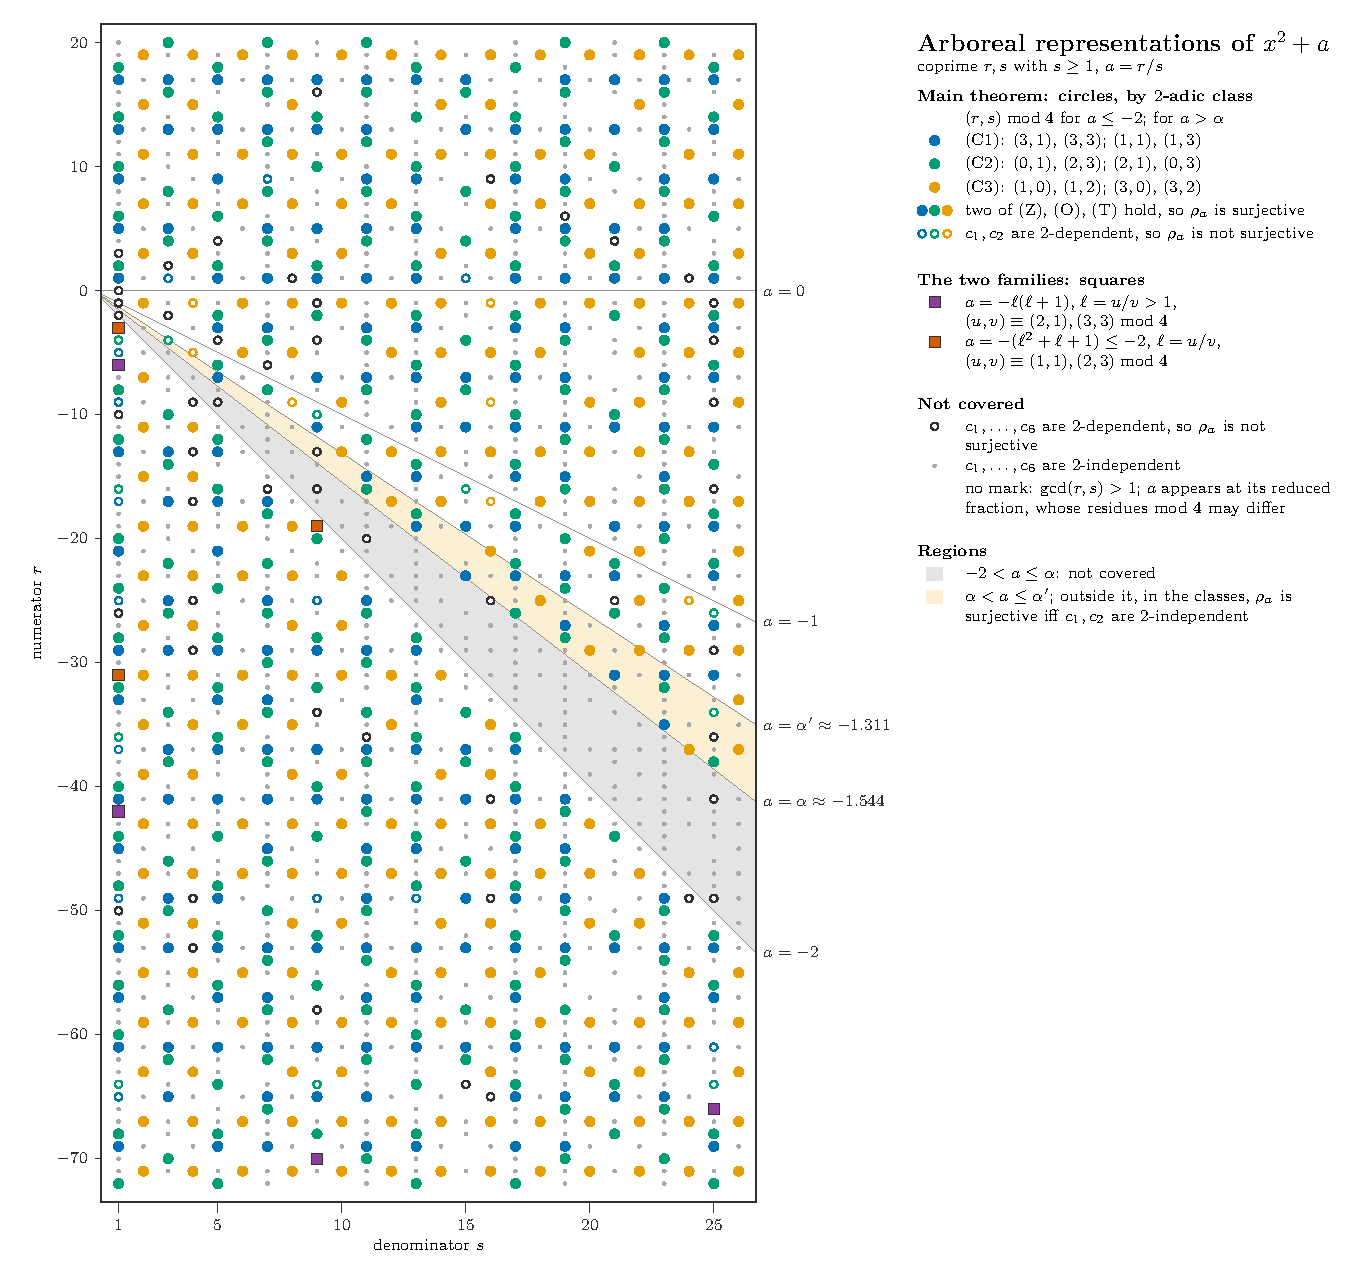
\includegraphics[width=\linewidth]{../../plots/coverage.pdf}}

% Items of a list are labelled (1), (2), ..., upright as in the paper, also when the label is
% given to \item, as in (C1). The web version does the same in templates/enumerate.jinja2s.
\setlist[enumerate,1]{label=(\arabic*)}
\setlist[enumerate]{font=\upshape}

% After \appendix, chapters are called "Appendix" and hyperref names their anchors by letters;
% Part II (\secondpart in macros/common.tex) has chapters again, with anchors of their own, and
% its longer numbers II.1, II.1.1 get wider boxes in the table of contents (tocloft).
\makeatletter
\newcommand{\restorechapters}{%
  \renewcommand{\@chapapp}{\chaptername}\renewcommand{\theHchapter}{II.\arabic{chapter}}%
  \addtocontents{toc}{\protect\setlength{\protect\cftchapnumwidth}{2.6em}%
    \protect\setlength{\protect\cftsecnumwidth}{3.4em}}}
\makeatother

\newcommand{\lean}[1]{}
\newcommand{\discussion}[1]{}
\newcommand{\leanok}{}
\newcommand{\mathlibok}{}
\newcommand{\notready}{}
% Make sure that arguments of \uses and \proves are real labels, by using invisible refs:
% latex prints a warning if the label is not defined, but nothing is shown in the pdf file.
% It uses LaTeX3 programming, this is why we use the expl3 package.
\ExplSyntaxOn
\NewDocumentCommand{\uses}{m}
 {\clist_map_inline:nn{#1}{\vphantom{\ref{##1}}}%
  \ignorespaces}
\NewDocumentCommand{\proves}{m}
 {\clist_map_inline:nn{#1}{\vphantom{\ref{##1}}}%
  \ignorespaces}
\ExplSyntaxOff


\title{When do all iterates of $x^2 + a$ have maximal Galois group? A blueprint}
\author{Michael Stoll}

\begin{document}
\maketitle
\tableofcontents
\chapter*{About this blueprint}
\addcontentsline{toc}{chapter}{About this blueprint}

This blueprint accompanies the paper~\cite{arboreal}, which gives simpler proofs of the main
results of~\cite{paper, li2020, li2021} on the surjectivity of the arboreal Galois representation
attached to~$x^2 + a$, working directly with the modified orbit~$(c_n)$ of~$0$ (with $c_1 = -a$)
and with quadratic characters of~$\QQ^\times$ instead of the Möbius quotients~$b_n$, and extends
them to rational parameters~$a$. It links each statement of the paper to its formalization in
Lean~4.

\emph{Organization.} Chapters~\ref{chap:intro}--\ref{chap:families} are the sections of the
paper, in the same order, and each of their statements carries the number it has in the paper.
The statements that the formalization needs beyond those of the paper come first in a chapter,
in a section \emph{Preliminaries}, and are numbered with letters (Lemma~5.A, \dots), so that the
paper's numbering is unaffected. Appendix~\ref{chap:criterion} proves
Proposition~\ref{prop:criterion}, which the paper quotes from~\cite{paper}.
Appendix~\ref{chap:further} collects further formalized results, among them the further criteria
mentioned at the end of Section~5 of the paper. Appendix~\ref{chap:auxiliary} contains the
general theory on which the Galois-theoretic part rests.

\emph{Status.} Every definition, lemma, proposition, theorem and corollary is formalized; the
question, the conjecture and the remarks are not statements of the formalization. Lean names are
given in \lname{typewriter} inside the statement or a \emph{Formalization} remark; the section
below describes the formalization.

\emph{Standing notation.} $a \in \QQ$, $f = X^2 + a$, $f_0 = X$ and $f_{n+1} = f_n^2 + a$ are
the iterates of~$f$ (written~$f^{\circ n}$ in the paper), $K_n \subseteq \Qbar$ is the splitting
field of~$f_n$ over~$\QQ$, and $\Om_n = \Gal(K_n/\QQ)$. $\Ct{n}$ denotes the~$n$-fold iterated
wreath product of~$C_2$ with itself. From Chapter~\ref{chap:phin} on, $a = r/s$ with coprime
integers~$r$, $s$ and $s \ge 1$.

\section*{The formalization}

\emph{Shared material.} The Galois-theoretic part --- the iterates, their splitting fields and
Galois groups, Odoni's embedding $\Om_n \hookrightarrow \Ct{n}$, the degree criterion and the
irreducibility lemma (the preliminaries of Chapter~\ref{chap:intro} and
Appendix~\ref{chap:criterion}), with the general theory of multiquadratic extensions, wreath
products and even polynomials it rests on (Appendix~\ref{chap:auxiliary}) --- is shared with the
formalization of~\cite{paper} along its own route, which also covers the order-theoretic facts
about~$(c_n)$ for $-2 \le a \le 0$ (Lemma~\ref{lem:sumsign}); none of it involves Möbius
inversion.

\emph{Devices.} Quadratic characters are Mathlib's \lname{MulChar ℚ ℤ} (a commutative group;
the value at~$0$ is~$0$, so $\chi(c_n) = -1$ carries $c_n \ne 0$ with it), and the characters
induced by Dirichlet characters come from Mathlib's \lname{quadraticChar (ZMod p)},
\lname{ZMod.χ₄} and \lname{ZMod.χ₈} through one construction (Definition~\ref{def:chars}).
The integer sequence~$w_n$ (Definition~\ref{def:wseq}) carries the arithmetic of
$c_n = r w_n/s^{2^{n-1}}$; for a modulus~$N$ prime to~$s$, the identity
$r w_n = s^{2^{n-1}} \bar c_n$ in~$\ZZ/N\ZZ$, with $(\bar c_n)$ the sequence of the parameter
$\bar a = r/s \bmod N$ (Lemma~\ref{lem:reduction}), turns every local argument into a
computation with the sequence $(\bar c_n)$ in~$\ZZ/N\ZZ$.

\emph{Layout.} The Galois-theoretic part is formalized in the directory \texttt{Galois} of
\texttt{QuadraticIterates/}, the characters of Chapter~\ref{chap:characters} in
\texttt{Characters}, the sequences~$(c_n)$ and~$(w_n)$ with their signs, orbits and valuations in
\texttt{Sequence}, the values of the characters along~$(c_n)$ in \texttt{Patterns}, and the
results of Chapters~\ref{chap:klein}--\ref{chap:families} and Appendix~\ref{chap:further} in
\texttt{Main}; Appendix~\ref{chap:auxiliary} is formalized in \texttt{EvenPoly.lean} and the
mirror files under \texttt{Mathlib/}. The repository's comparator challenges state the main
result of Section~3 of~\cite{paper} (one challenge per case), the theorems
of~\cite{li2020, li2021} (Theorem~3.3 of~\cite{li2021} in the stronger form of
Corollary~\ref{cor:li2021}), and the parts (1), (2)(a)--(d) and (2)(e) of
Theorem~\ref{thm:main} together with Corollary~\ref{cor:interval}; the challenges reproduce the
definitions of the~$2$-adic classes and of the lists of conditions.

\chapter{Introduction}
\label{chap:intro}

\section{Preliminaries}
\supporting

The paper works with the arboreal representation~$\rho_a$ on the tree of preimages of~$0$; the
formalization works with the Galois groups of the iterates, which are its images on the finite
levels. These are the objects in the statement of Proposition~\ref{prop:criterion}.

\begin{definition}[The iterates~$f_n$]
  \label{def:iterates}
  \lean{QuadraticIterates.iteratedPoly, QuadraticIterates.iteratedPoly_zero,
    QuadraticIterates.iteratedPoly_one, QuadraticIterates.iteratedPoly_succ,
    QuadraticIterates.iteratedPoly_succ_comp, QuadraticIterates.eval_zero_iteratedPoly_succ,
    QuadraticIterates.map_iteratedPoly, QuadraticIterates.aeval_ratCast_iteratedPoly,
    QuadraticIterates.monic_iteratedPoly, QuadraticIterates.natDegree_iteratedPoly,
    QuadraticIterates.iteratedPoly_zero_left,
    QuadraticIterates.ncard_rootSet_iteratedPoly_le}
  \leanok
  $f_0 := X$ and $f_{n+1} := f_n^2 + a$. These are monic of degree~$2^n$, so~$f_n$ has at
  most~$2^n$ roots, and $f_{n+1} = f_n \circ (X^2 + a)$; so $f_n = f^{\circ n}$.
  \formalnote{\lname{iteratedPoly} is defined over any commutative semiring; over~$\QQ$ it is
  written \texttt{f}$\QQ$\texttt{[a, n]}.}
\end{definition}

\begin{definition}[The fields~$K_n$ and the groups~$\Om_n$]
  \label{def:galois}
  \uses{def:iterates}
  \lean{QuadraticIterates.splittingField, QuadraticIterates.GaloisGroup,
    QuadraticIterates.splittingField.instIsSplittingField,
    QuadraticIterates.splittingField.instFiniteDimensional,
    QuadraticIterates.splittingField.instIsGalois,
    QuadraticIterates.splittingField_zero_eq_bot,
    QuadraticIterates.card_galoisGroup_eq_finrank}
  \leanok
  For $a \in \QQ$, $K_n \subseteq \Qbar$ is the subfield generated by the roots of~$f_n$, and
  $\Om_n = \Gal(f_n/\QQ)$. One has $K_0 = \QQ$ and $\#\Om_n = [K_n : \QQ]$.
  \formalnote{$K_n$ is an \lname{IntermediateField} of \lname{AlgebraicClosure ℚ}, so that the
  tower $K_n \subseteq K_{n+1}$ is an inclusion of subfields of one field and relative degrees
  are \lname{IntermediateField.relfinrank}; $\Om_n$ is Mathlib's \lname{Polynomial.Gal}.}
\end{definition}

\begin{definition}[The iterated wreath power~$\Ct{n}$]
  \label{def:wreath}
  \lean{QuadraticIterates.WreathPower, QuadraticIterates.card_wreathPower}
  \leanok
  $\Ct{n}$ is the~$n$-fold iterated regular wreath product of~$C_2$ with itself; it has order
  $2^{2^n - 1}$.
  \formalnote{Mathlib's \lname{IteratedWreathProduct} of \lname{Multiplicative (ZMod 2)}.
  ``$\Om_n \cong \Ct{n}$'' is \lname{Nonempty (GaloisGroup a n ≃* WreathPower n)}, and
  ``$\rho_a$ is surjective'' is the statement that this holds for all~$n$.}
\end{definition}

\section{The question and the sequence \texorpdfstring{$(c_n)$}{(c\_n)}}
\paperitems

Let $a \in \QQ$ be nonzero and $f = f_a = x^2 + a$. If no iterate has multiple roots, the pairs
$(n, \xi)$ with~$\xi$ a root of~$f^{\circ n}$ in a fixed algebraic closure of~$\QQ$ form an infinite
complete binary tree~$T$, in which $(n + 1, \eta)$ is a child of $(n, \xi)$ when $\xi = f(\eta)$.
The absolute Galois group~$\Gal_{\QQ}$ of~$\QQ$ acts on~$T$ by tree automorphisms, which gives the
\emph{arboreal Galois representation} $\rho_a \colon \Gal_{\QQ} \to \operatorname{Aut}(T)$. An
iterate~$f^{\circ n}$ has multiple roots if and only if~$0$ is a root of~$f^{\circ m}$ for some
$1 \le m \le n$; so some iterate has multiple roots if and only if~$0$ is periodic under~$f$,
which for $a \in \QQ$ happens exactly when $a \in \{-1, 0\}$ (Remark~\ref{rem:nonzero}).

\begin{question}
  For which $a \in \QQ$ is~$\rho_a$ surjective?
\end{question}

This is equivalent to the surjectivity, for every~$n$, of the action~$\rho_a^n$ on the finite
tree~$T_n$ of the levels up to~$n$. The automorphism group of~$T_n$ is a Sylow~$2$-subgroup of
the symmetric group on its~$2^n$ leaves, isomorphic to the~$n$th wreath power~$\Ct{n}$ of~$C_2$,
and the image of~$\rho^n_a$ is~$\Om_n$. So~$\rho^n_a$ is surjective if and only if
$\Om_n \cong \Ct{n}$ (Definitions~\ref{def:galois} and~\ref{def:wreath}). The question was first
asked by J.~McKay for $a = 1$; see~\cite{odoni}. Odoni's earlier paper~\cite{odoni1985} sets up
some general theory, and the survey~\cite{jones} describes what is known or expected on this and
related questions.

\begin{definition}[The sequence~$c_n$]
  \label{def:cseq}
  \uses{def:iterates, def:gammaseq}
  \lean{QuadraticIterates.cSeq, QuadraticIterates.cSeq_zero, QuadraticIterates.cSeq_one,
    QuadraticIterates.cSeq_succ, QuadraticIterates.cSeq_two,
    QuadraticIterates.cSeq_succ_eq_neg_one_pow_mul_eval,
    QuadraticIterates.cSeq_succ_eq_neg_one_pow_mul_eval_zero, QuadraticIterates.map_cSeq,
    QuadraticIterates.intCast_cSeq, QuadraticIterates.ratCast_cSeq}
  \leanok
  Define the sequence $(c_n)_{n \ge 0}$ of rational numbers by
  \[ c_0 = 0, \qquad c_1 = -a, \qquad c_{n+1} = f(c_n) = c_n^2 + a \quad \text{for $n \ge 1$.} \]
  This is the orbit of~$0$ under~$f$, \emph{except} that the sign of~$c_1$ is changed (note
  $f(-a) = f(a)$). Thus $c_{n+1} = f_n(a)$ for all~$n$, $c_n = f_n(0)$ for $n \ge 2$, and
  $c_1 = -f_1(0)$.
  \formalnote{\lname{cSeq} is defined for a parameter in any commutative ring, as the
  sequence \lname{gammaSeq} of the even polynomial~$X^2 + a$ with first term~$-a$
  (Definition~\ref{def:gammaseq}); it commutes with ring homomorphisms
  (\lname{map\_cSeq}). This is used with the rings~$\QQ$ and~$\ZZ/N\ZZ$.}
\end{definition}

\begin{remark}[Vanishing terms]
  \label{rem:nonzero}
  $c_n = 0$ for some $n \ge 1$ holds if and only if~$0$ is periodic under~$f$. For $a \in \QQ$,
  this is the case if and only if $a \in \{-1, 0\}$. If~$p$ divides the denominator of~$a$, then
  the~$p$-adic valuation doubles in each step, so~$0$ cannot be periodic; so~$a$ must be an
  integer. For $a \ge 1$ or $a \le -3$ the orbit tends to infinity, leaving $a \in \{-2, -1, 0\}$;
  and for $a = -2$, $0$ is preperiodic ($0 \mapsto -2 \mapsto 2 \mapsto 2$), not periodic.
  \formalnote{The equivalence with $a \in \{0, -1\}$ is \lname{exists\_cSeq\_eq\_zero\_iff}, with
  \lname{cSeq\_ne\_zero} for $a \notin \{-1, 0\}$; both are listed under Lemma~\ref{lem:vp},
  which uses them. The periodicity of~$0$ is not formalized. Most statements do not need the
  remark, as a character with $\chi(c_n) = -1$ already forces $c_n \ne 0$.}
\end{remark}

The~$p$-adic valuations along $(c_n)_{n \ge 1}$ behave as follows.

\begin{lemma}[Rigid divisibility]
  \label{lem:rigid}
  \uses{def:cseq}
  \lean{QuadraticIterates.cSeq_sq_dvd_cSeq_mul_sub, QuadraticIterates.sq_dvd_cSeq_sub,
    QuadraticIterates.cSeq_mul_of_sq_eq_zero, QuadraticIterates.cSeq_eq_self_of_sq_eq_zero,
    QuadraticIterates.cSeq_add_eq_of_sq_eq_zero, QuadraticIterates.cSeq_add_mul_eq_of_sq_eq_zero,
    QuadraticIterates.cSeq_add_eq_of_add_eq, QuadraticIterates.cSeq_add_mul_eq_of_add_eq}
  \leanok
  Let~$p$ be a prime and assume that~$a$ is a~$p$-adic integer. Then~$c_n$ is a~$p$-adic integer
  for all~$n$, and in~$\ZZ_p$ we have $c_{mk} \equiv c_m \bmod c_m^2$ for all $m \ge 2$ and
  $k \ge 1$, and similarly $c_k \equiv -c_1 = a \bmod c_1^2$ for all $k \ge 2$.
  \formalnote{For a parameter in any commutative ring~$R$ (such as~$\ZZ_p$), where the integrality
  is automatic: \lname{cSeq\_sq\_dvd\_cSeq\_mul\_sub} and \lname{sq\_dvd\_cSeq\_sub}. They are the
  images of the ring statements in $R/(c_m^2)$: if $c_m^2 = 0$ ($m \ge 1$), the sequence
  is~$m$-periodic from $n = 2$ on (\lname{cSeq\_add\_eq\_of\_sq\_eq\_zero}), so $c_{mk} = c_m$ for
  $m \ge 2$ (\lname{cSeq\_mul\_of\_sq\_eq\_zero}) and $c_k = a$ for $m = 1$
  (\lname{cSeq\_eq\_self\_of\_sq\_eq\_zero}).}
\end{lemma}
\begin{proof}
  \leanok
  Since $f = x^2 + a$ is even, so is~$f^{\circ n}$ for $n \ge 1$, so
  $f^{\circ n}(z) \equiv f^{\circ n}(0) \bmod z^2$. Fix $m \ge 2$; then $c_m = f^{\circ m}(0)$, and
  by induction on~$k$,
  \[ c_{m(k+1)} = f^{\circ (mk)}(c_m) \equiv f^{\circ (mk)}(0) = c_{mk} \bmod c_m^2. \]
  The case $m = 1$ is similar, using $c_2 = f(c_1) \equiv f(0) = -c_1 \bmod c_1^2$. The
  formalization argues in $\bar R = R/(c_m^2)$, where $\bar c_m^2 = 0$, so
  $\bar c_{m+1} = \bar a$ and $\bar c_{m+2} = \bar a^2 + \bar a = \bar c_2$; periodicity then
  propagates along the recursion from $n = 2$ on.
\end{proof}

\begin{lemma}[The~$p$-adic valuations along~$(c_n)$]
  \label{lem:vp}
  \uses{lem:rigid, def:wseq, lem:reduction, lem:wseq-res, lem:wseq-mul, lem:signs}
  \lean{QuadraticIterates.padicValRat_cSeq_trichotomy,
    QuadraticIterates.padicValRat_cSeq_of_padicValRat_neg,
    QuadraticIterates.padicValRat_cSeq_of_dvd_left, QuadraticIterates.padicValRat_cSeq_eq_ite,
    QuadraticIterates.padicValRat_cSeq_eq_padicValInt, QuadraticIterates.padicValInt_wSeq_eq_ite,
    QuadraticIterates.dvd_wSeq_iff, QuadraticIterates.cSeq_eq_zero_iff_dvd,
    QuadraticIterates.cSeq_ne_zero, QuadraticIterates.exists_cSeq_eq_zero_iff}
  \leanok
  Let~$p$ be a prime and assume that $a \notin \{-1, 0\}$. Then exactly one of the following
  possibilities holds.
  \begin{enumerate}
    \item For all $n \ge 1$, $v_p(c_n) = 0$.
    \item There are $m_p, e_p \in \ZZ_{\ge 1}$ such that $v_p(c_n) = 0$ if $m_p \nmid n$, and
          $v_p(c_n) = e_p$ if $n \ge 1$ and $m_p \mid n$.
    \item There is $e_p \in \ZZ_{< 0}$ such that $v_p(c_n) = 2^{n-1} e_p$ for all $n \ge 1$.
  \end{enumerate}
  \formalnote{\lname{padicValRat\_cSeq\_trichotomy} states that one of the three holds; that at
  most one does is clear from the values at $n = 1$ and $n = m_p$, and is not stated. For
  $a = r/s$, the cases are those of \lname{padicValRat\_cSeq\_of\_padicValRat\_neg} ($p \mid s$,
  $e_p = v_p(a)$), \lname{padicValRat\_cSeq\_of\_dvd\_left} ($p \mid r$, $m_p = 1$,
  $e_p = v_p(r)$) and \lname{padicValRat\_cSeq\_eq\_ite} ($p \nmid rs$, with~$m_p$ the first
  index with $p \mid w_{m_p}$ and $e_p = v_p(w_{m_p})$).}
\end{lemma}
\begin{proof}
  \leanok
  If $v_p(a) < 0$, then $v_p(c_n^2) < v_p(a)$ and so $v_p(c_{n+1}) = 2 v_p(c_n)$; this is the
  third case with $e_p = v_p(a)$. If $v_p(a) \ge 0$, then $v_p(c_n) \ge 0$ for all~$n$
  (Lemma~\ref{lem:rigid}). If $v_p(c_n) = 0$ for all $n \ge 1$, we are in the first case.
  Otherwise let $m_p = \min\{m \ge 1 : v_p(c_m) > 0\}$ and $e_p = v_p(c_{m_p})$: the sequence
  modulo~$p$, starting from~$0$, is periodic with period~$m_p$, and Lemma~\ref{lem:rigid} with
  $m = m_p$ gives $v_p(c_{k m_p}) = e_p$. Compare the proof of~\cite{paper}, Lemma~1.1(b).

  The formalization writes $a = r/s$ and $c_n = r w_n / s^{2^{n-1}}$ (Lemma~\ref{lem:reduction}).
  For $p \nmid s$, $v_p(c_n) = v_p(r w_n)$, and~$w_n$ is prime to~$r$ and to~$s$
  (Lemma~\ref{lem:wseq-res}); this settles $p \mid r$. For $p \nmid rs$, modulo~$p$ the vanishing
  of~$\bar c_n$ is that of~$w_n$; if~$m$ is the first index with $\bar c_m = 0$, then
  $\bar c_n = 0$ if and only if $m \mid n$ (\lname{cSeq\_eq\_zero\_iff\_dvd}), and
  $w_{mk} = w_m T$ with $T \equiv s^{2^{mk-1} - 2^{m-1}} \bmod w_m$ prime to~$p$
  (Lemma~\ref{lem:wseq-mul}). The terms are nonzero by Remark~\ref{rem:nonzero}: for
  non-integral~$a$ by the third case, for integral $a \notin \{-1, 0\}$ because $a > 0$ or
  $a \le -2$ and Lemma~\ref{lem:signs} applies.
\end{proof}

\begin{definition}[$2$-independence]
  \label{def:twoindep}
  \lean{QuadraticIterates.TwoIndependent, QuadraticIterates.TwoIndependent.ne_zero,
    QuadraticIterates.TwoIndependent.not_isSquare,
    QuadraticIterates.twoIndependent_iff_linearIndependent,
    QuadraticIterates.TwoIndependent.of_snoc, QuadraticIterates.twoIndependent_snoc_iff,
    QuadraticIterates.TwoIndependent.comp, QuadraticIterates.twoIndependent_iff_forall_fin,
    QuadraticIterates.twoIndependent_iff_forall_finset,
    Fin.exists_eq_map_castSuccEmb_or_insert_last, sqClass}
  \leanok
  A family $(r_i)_{i \in I}$ of rational numbers is \emph{$2$-independent} if for every finite
  subset $S \subseteq I$, $\prod_{i \in S} r_i$ is a square only when $S = \emptyset$. Otherwise
  the family is \emph{$2$-dependent}. (When all~$r_i$ are nonzero, this says that the images of
  the~$r_i$ in $\QQ^\times/\QQ^{\times 2}$ are linearly independent over~$\FF_2$.) A family
  containing zero is~$2$-dependent.
  \formalnote{\lname{TwoIndependent} is stated for a family in any commutative monoid; the
  translation into linear independence of the classes \lname{sqClass} in $L^\times/L^{\times 2}$
  holds for any field~$L$. The family $c_1, \dots, c_n$ is $i \mapsto c_{i+1}$ on \lname{Fin n}.}
\end{definition}

The following is the equivalence ``a) $\Leftrightarrow$ b)'' in part~1) of the Theorem in
Section~1 of~\cite{paper}.

\begin{proposition}[Stoll's criterion]
  \label{prop:criterion}
  \uses{def:galois, def:wreath, def:twoindep, def:cseq}
  \lean{QuadraticIterates.nonempty_mulEquiv_iff_twoIndependent,
    QuadraticIterates.irreducible_iteratedPoly_of_twoIndependent,
    QuadraticIterates.forall_nonempty_mulEquiv_iff_twoIndependent}
  \leanok
  Fix $a \in \QQ$ and $n \in \ZZ_{\ge 1}$. Then~$\rho^n_a$ is defined and surjective if and only
  if $(c_1, \dots, c_n)$ is~$2$-independent. Consequently, $\rho_a$ is defined and surjective if
  and only if the family $(c_n)_{n \ge 1}$ is~$2$-independent.
  \formalnote{Stated as $\Om_n \cong \Ct{n}$ if and only if $c_1, \dots, c_n$
  are~$2$-independent, for every $n \ge 0$ (\lname{nonempty\_mulEquiv\_iff\_twoIndependent}), and
  for all~$n$ at once (\lname{forall\_nonempty\_mulEquiv\_iff\_twoIndependent}, with the family
  \lname{fun n : ℕ ↦ cSeq a (n + 1)}).}
\end{proposition}
\begin{proof}
  \leanok
  \uses{lem:criterion-irr, lem:irred, lem:irred-of-iso}
  The proof is the subject of Appendix~\ref{chap:criterion}. By
  Lemma~\ref{lem:criterion-irr} it suffices that $f_0, \dots, f_n$ are irreducible under either
  hypothesis. If $c_1, \dots, c_n$ are~$2$-independent, none of them is a square, and
  Lemma~\ref{lem:irred} applies; if $\Om_n \cong \Ct{n}$, Lemma~\ref{lem:irred-of-iso} does. For
  the second statement, a finite subset of $\{1, 2, \dots\}$ lies in some $\{1, \dots, n\}$.
\end{proof}

\cite{paper} defines~$2$-independence only for families of nonzero numbers and assumes that~$-a$
is not a square (which implies that all~$c_n$ are nonzero). The statement remains true in the
general form above: when~$-a$ is a square, $\rho^1_a$ is not surjective, hence neither
is~$\rho^n_a$ for $n \ge 1$, and $c_1 = -a$ is a square, so $(c_1, \dots, c_n)$ is~$2$-dependent.
This includes $a = 0$ and $a = -1$, where~$\rho_a$ is not defined. So the approach is to show
that $(c_n)_{n \ge 1}$ is~$2$-independent for $a \in \QQ$ with suitable properties.

The proofs in~\cite{paper, li2020, li2021} follow~\cite{odoni} in considering instead the
sequence~$(b_n)$ obtained from~$(c_n)$ by multiplicative Möbius inversion. When
$a \in \ZZ \setminus \{-1, 0\}$, $(c_n)$ is a rigid divisibility sequence in~$\ZZ$
(Lemma~\ref{lem:vp}), so the~$b_n$ are pairwise coprime integers; $(c_n)_{n \ge 1}$
is~$2$-independent if and only if $(b_n)_{n \ge 1}$ is, and this follows if~$|b_n|$ is never a
square for $n \ge 2$ and~$b_1$ is not a square. That gives a simpler criterion --- single terms
instead of arbitrary finite products --- at the price of more complicated objects. The paper
shows that the results of~\cite{paper, li2020, li2021} are obtained as easily by working
directly with~$(c_n)$, and extends them to rational parameters. Its main result
(Theorem~\ref{thm:main}) is that for essentially half of all rational~$a$ outside the interval
$(-2, \alpha)$, with~$\alpha$ the real root of $x^3 + 2x^2 + 2x + 2$, $\rho_a$ is surjective as
soon as (and therefore if and only if) $\rho_a^2$ is, that is, as soon as none of~$-a$,
$a^2 + a$ and $-a(a^2 + a)$ is a square.

\chapter{Quadratic characters and the criterion}
\label{chap:characters}

\section{Quadratic characters of \texorpdfstring{$\QQ$}{Q}}

\begin{definition}[Quadratic characters]
  \label{def:qchar}
  \lean{MulChar.apply_eq_one_or_eq_neg_one, MulChar.isQuadratic_int,
    MulChar.apply_ne_neg_one_of_isSquare, MulChar.apply_inv, MulChar.apply_div, MulChar.apply_sq,
    MulChar.apply_mul_sq, MulChar.apply_div_sq}
  \leanok
  A \emph{quadratic character} of $\QQ$ is a homomorphism $\chi \colon \QQ^\times \to \{\pm 1\}$,
  extended to $\QQ$ by $\chi(0) = 0$. Equivalently, a multiplicative map $\chi \colon \QQ \to \ZZ$
  with $\chi(1) = 1$ and $\chi(0) = 0$; its values on $\QQ^\times$ are units of $\ZZ$, i.e.\
  $\pm 1$. Quadratic characters form a group under pointwise multiplication, and
  $\chi(x y^2) = \chi(x)$ for $y \ne 0$; in particular $\chi(x) \ne -1$ when $x$ is a square, and
  $\chi(1/x) = \chi(x)$.
  \formalnote{Mathlib's \lname{MulChar ℚ ℤ}, a \lname{CommGroup}; it corresponds to
  \lname{ℚˣ →* ℤˣ} by \lname{MulChar.equivToUnitHom}, i.e.\ to the characters of
  $\QQ^\times/\QQ^{\times 2}$. The general lemmas are stated for a character with values in $\ZZ$
  of a commutative monoid (\lname{MulChar.apply\_eq\_one\_or\_eq\_neg\_one} at units, so every
  such character is quadratic) or of a commutative group with zero (\lname{MulChar.apply\_inv},
  \lname{MulChar.apply\_div}, \lname{MulChar.apply\_mul\_sq}, \lname{MulChar.apply\_div\_sq}).
  \lname{MulChar.apply\_ne\_neg\_one\_of\_isSquare}, for values in an ordered ring, is the whole
  reason a character detects non-squares: $\chi(y^2) = \chi(y)^2 \ge 0$.}
\end{definition}

\begin{definition}[The characters used]
  \label{def:chars}
  \uses{def:qchar}
  \lean{Rat.mulCharOfInt, Rat.mulCharOfInt_apply, Rat.mulCharOfInt_intCast,
    Rat.map_num_mul_map_den_mul, Rat.signChar, Rat.signChar_apply, Rat.signChar_apply_of_pos,
    Rat.signChar_apply_of_neg, Rat.valChar, Rat.valChar_intCast, Rat.unitPartChar,
    Rat.unitPartChar_intCast, Rat.unitPartChar_natCast_self, ZMod.isUnit_intCast_of_not_dvd}
  \leanok
  For $x \in \QQ^\times$ and a prime $p$ let $x_p = p^{-v_p(x)} x$ be the prime-to-$p$ part.
  \begin{enumerate}
    \item $\sgn(x)$, the sign.
    \item $\val_p(x) = (-1)^{v_p(x)}$, for a prime $p$.
    \item For a prime $p$, a power $N$ of $p$ and a character $\psi$ of $(\ZZ/N\ZZ)^\times$ with
          values $\pm 1$ (extended by $0$ to $\ZZ/N\ZZ$): $\chi_\psi(x) = \psi(x_p \bmod N)$,
          where $x_p$ is reduced modulo $N$ as a fraction with denominator prime to $p$.
          Special cases:
          $\chi_p = \chi_\psi$ for an odd prime $p$, $N = p$ and $\psi$ the Legendre symbol;
          $\chi_4 = \chi_\psi$ for $N = 4$ and $\psi(-1) = -1$;
          $\chi_8 = \chi_\psi$ for $N = 8$ and $\psi(\pm 1) = 1$, $\psi(\pm 3) = -1$.
  \end{enumerate}
  Then $\chi_\psi(p) = 1$, and $\chi_\psi(m) = \psi(m \bmod N)$ for an integer $m$ prime to $p$;
  more generally $\chi_\psi(m/k) = \psi(m)\psi(k)$ for integers $m$, $k$ prime to $p$.
  We call $\val_p$, $\chi_p$ (resp.\ $\val_2$, $\chi_4$, $\chi_8$) and their products the
  \emph{characters at $p$}; they are induced by the characters of $\QQ_p^\times/\QQ_p^{\times 2}$.
  \formalnote{In the mirror file \lname{QuadraticIterates/Mathlib/NumberTheory/MulChar/Rat.lean}.
  All three are extensions $x \mapsto f(\mathrm{num}\,x) f(\mathrm{den}\,x)$ of multiplicative
  functions $f$ on $\ZZ$ that are $\pm 1$ at nonzero integers (\lname{Rat.mulCharOfInt}):
  \lname{Rat.signChar}, \lname{Rat.valChar p} and \lname{Rat.unitPartChar p ψ}, the last one
  defined for any \lname{ψ : MulChar (ZMod N) ℤ}, through $\psi(\operatorname{sign}(m) \cdot
  |m|/p^{v_p(m)})$, with value lemmas for $N = p^k$: \lname{Rat.unitPartChar\_intCast}
  ($p \nmid m$) and \lname{Rat.unitPartChar\_natCast\_self} ($\chi_\psi(p) = 1$). The value at
  $m/k$ follows from \lname{MulChar.apply\_div}. $\chi_p$, $\chi_4$, $\chi_8$ are
  \lname{Rat.unitPartChar} of \lname{quadraticChar (ZMod p)}, \lname{ZMod.χ₄} and \lname{ZMod.χ₈}.}
\end{definition}

\section{Patterns}

\begin{definition}[Patterns]
  \label{def:pattern}
  \uses{def:qchar}
  \lean{QuadraticIterates.HasCharPattern, QuadraticIterates.HasCharPattern.mul,
    QuadraticIterates.HasCharPattern.mono, QuadraticIterates.HasCharPattern.congr}
  \leanok
  Let $(v_m)_{m \ge 1}$ be a sequence of rational numbers, $n \ge 1$ and
  $\varepsilon \colon \ZZ_{\ge n} \to \{\pm 1\}$. The \emph{pattern $\varepsilon$ is realized
  from $n$} if some quadratic character $\chi$ satisfies $\chi(v_m) = \varepsilon_m$ for all
  $m \ge n$. Patterns realized from $n$ are closed under pointwise products (multiply the
  characters), contain the constant pattern $1$ if all $v_m$ are nonzero (the trivial
  character), and a pattern realized
  from $n$ is realized from every $n' \ge n$. We write patterns as strings of signs:
  $\chi(v_\bullet) = ({+}{-}{-}\cdots)$.
  \formalnote{\lname{HasCharPattern (v : ℕ → M) (n : ℕ) (ε : ℕ → ℤ) : Prop :=
  ∃ χ : MulChar M ℤ, ∀ m ≥ n, χ (v m) = ε m}, for a sequence in a commutative monoid $M$, with
  \lname{HasCharPattern.congr} for patterns agreeing from $n$ on. Values of $\varepsilon$ before
  $n$ are irrelevant. The constant pattern $1$ is not needed.}
\end{definition}

\begin{definition}[$\phi_n$, $\phi_0$ and $\tau$]
  \label{def:phin}
  \uses{def:pattern, def:cseq}
  \leanok
  For the sequence $(c_m)$ of $a \in \QQ$:
  \begin{itemize}
    \item $a$ \emph{has $\phi_n$} ($n \ge 1$) if the pattern $-1$ at $n$, $+1$ after $n$ is
          realized from $n$: a character $\phi_n$ with $\phi_n(c_n) = -1$ and
          $\phi_n(c_m) = 1$ for all $m > n$;
    \item $a$ \emph{has $\phi_0$} if the constant pattern $-1$ is realized from $1$:
          $\phi_0(c_m) = -1$ for all $m \ge 1$;
    \item $a$ \emph{has $\tau$} if the pattern $({+}{-}{-}\cdots)$ is realized from $1$:
          $\tau(c_1) = 1$ and $\tau(c_m) = -1$ for all $m \ge 2$.
  \end{itemize}
  \formalnote{The patterns are \lname{Pi.mulSingle n (-1)}, the constant \lname{-1} and
  \lname{-Pi.mulSingle 1 (-1)}; statements are written with \lname{HasCharPattern (cSeq a)}
  directly, without further definitions.}
\end{definition}

\section{The criterion}

\begin{proposition}[The criterion with characters]
  \label{prop:crit}
  \uses{def:pattern, def:twoindep}
  \lean{QuadraticIterates.twoIndependent_of_forall_hasCharPattern,
    QuadraticIterates.forall_nonempty_mulEquiv_of_forall_hasCharPattern}
  \leanok
  Let $(v_m)_{m \ge 1}$ be a sequence of rational numbers such that for every $n \ge 1$ the pattern
  $-1$ at $n$, $+1$ after $n$ is realized from $n$. Then $(v_m)_{m \ge 1}$ is $2$-independent.
  In particular, if $a$ has $\phi_n$ for every $n \ge 1$, then $(c_n)_{n \ge 1}$ is
  $2$-independent and $\rho_a$ is surjective.
  \formalnote{For a sequence in any commutative monoid, with conclusion
  \lname{TwoIndependent (fun m : ℕ ↦ v (m + 1))}.}
\end{proposition}
\begin{proof}
  \leanok
  \uses{thm:criterion-infinite}
  Let $S \subseteq \ZZ_{\ge 1}$ be finite and nonempty, $n = \min S$, and $\phi_n$ as in the
  hypothesis. Then $\phi_n(\prod_{k \in S} v_k) = \phi_n(v_n) \prod_{k \in S, k > n}
  \phi_n(v_k) = -1$, so the product is not a square (Definition~\ref{def:qchar}). The second
  statement follows with Theorem~\ref{thm:criterion-infinite}.
\end{proof}

\begin{lemma}[Characters from linear forms]
  \label{lem:dual}
  \uses{def:qchar, def:twoindep}
  \lean{QuadraticIterates.mulCharOfDual, QuadraticIterates.mulCharOfDual_apply}
  \leanok
  Let $f \colon \QQ^\times/\QQ^{\times 2} \to \FF_2$ be $\FF_2$-linear. Then
  $x \mapsto (-1)^{f([x])}$ on $\QQ^\times$, $0 \mapsto 0$, is a quadratic character.
  If $V$ is a subspace of $\QQ^\times/\QQ^{\times 2}$ and $[x] \notin V$, there is such an $f$
  with $f([x]) = 1$ and $f(V) = 0$.
  \formalnote{For any field $K$ in place of $\QQ$, with \lname{SquareClasses K} and
  \lname{sqClass}: \lname{mulCharOfDual (f : Module.Dual (ZMod 2) (SquareClasses K)) :
  MulChar K ℤ}; the separation is Mathlib's
  \lname{Submodule.exists\_dual\_map\_eq\_bot\_of\_notMem} (every module over a field is free).}
\end{lemma}
\begin{proof}
  \leanok
  The map is the composition of the class map, $f$, and the isomorphism
  $\FF_2 \cong \{\pm 1\}$; vector spaces over a field have enough linear forms to separate a
  vector from a subspace.
\end{proof}

\begin{proposition}[The converse]
  \label{prop:crit-converse}
  \uses{lem:dual}
  \lean{QuadraticIterates.hasCharPattern_of_twoIndependent}
  \leanok
  If $(v_m)_{m \ge 1}$ is $2$-independent, then for every $n \ge 1$ the pattern $-1$ at $n$,
  $+1$ after $n$ is realized from $n$.
  \formalnote{For a sequence in a field. The classes of $v_1, v_2, \dots$ are linearly
  independent (\lname{twoIndependent\_iff\_linearIndependent} holds for families indexed by any
  type), and \lname{LinearIndependent.notMem\_span\_image} gives $[v_n] \notin V$.}
\end{proposition}
\begin{proof}
  \leanok
  \uses{lem:dual, def:twoindep}
  All $v_m$ are nonzero. If $[v_n]$ lay in the span of the $[v_m]$, $m > n$, then $v_n$ times a
  finite product of later terms would be a square, contradicting $2$-independence. So
  Lemma~\ref{lem:dual} gives $f$ with $f([v_n]) = 1$ and $f([v_m]) = 0$ for $m > n$, and the
  character $(-1)^f$ realizes the pattern.
\end{proof}

\begin{theorem}[The criterion]
  \label{thm:tfae}
  \uses{thm:criterion-infinite, prop:crit, prop:crit-converse}
  For $a \in \QQ$ the following are equivalent:
  \begin{enumerate}
    \item $\Om_n \cong \Ct{n}$ for all $n$, i.e.\ $\rho_a$ is surjective;
    \item $(c_n)_{n \ge 1}$ is $2$-independent;
    \item $a$ has $\phi_n$ for every $n \ge 1$.
  \end{enumerate}
  \lean{QuadraticIterates.tfae_forall_nonempty_mulEquiv}
  \leanok
\end{theorem}
\begin{proof}
  \leanok
  \uses{thm:criterion-infinite, prop:crit, prop:crit-converse}
  (1)$\iff$(2) is Theorem~\ref{thm:criterion-infinite}, (3)$\Rightarrow$(2) is
  Proposition~\ref{prop:crit}, (2)$\Rightarrow$(3) is Proposition~\ref{prop:crit-converse}.
\end{proof}

\section{Combining characters}

The lemmas of this section produce $\phi_n$ from simpler patterns by multiplying characters.

\begin{lemma}[Two of three]
  \label{lem:klein}
  \uses{def:phin}
  \lean{QuadraticIterates.hasCharPattern_neg_mulSingle_of_neg_of_mulSingle,
    QuadraticIterates.hasCharPattern_mulSingle_of_neg_of_neg_mulSingle,
    QuadraticIterates.hasCharPattern_neg_of_mulSingle_of_neg_mulSingle}
  \leanok
  If $a$ has two of $\phi_0$, $\phi_1$, $\tau$, it has the third.
  \formalnote{The patterns $({-}{-}{-}\cdots)$, $({-}{+}{+}\cdots)$, $({+}{-}{-}\cdots)$ are the
  non-trivial elements of a Klein four-group under pointwise multiplication; three one-line
  consequences of \lname{HasCharPattern.mul}, stated for \lname{Pi.mulSingle k (-1)} with any
  $k$ and from any $n$.}
\end{lemma}
\begin{proof}
  \leanok
  The product of the patterns of any two of $\phi_0$, $\phi_1$, $\tau$ is the pattern of the
  third.
\end{proof}

\begin{lemma}[A jump after $n$]
  \label{lem:jump}
  \uses{def:phin}
  \lean{QuadraticIterates.hasCharPattern_mulSingle_of_neg_of_forall_lt}
  \leanok
  Let $n \ge 1$. If $a$ has $\phi_0$ and some character $\psi$ satisfies $\psi(c_n) \ne 0$ and
  $\psi(c_m) = -\psi(c_n)$ for all $m > n$, then $a$ has $\phi_n$.
\end{lemma}
\begin{proof}
  \leanok
  Take $\phi_n = \psi$ if $\psi(c_n) = -1$ and $\phi_n = \phi_0 \psi$ if $\psi(c_n) = 1$.
\end{proof}

\begin{lemma}[A period-two jump]
  \label{lem:jump2}
  \uses{def:phin}
  \lean{QuadraticIterates.hasCharPattern_mulSingle_of_neg_of_alternating}
  \leanok
  Let $n \ge 1$. Assume that $a$ has $\phi_0$, that some character $\psi$ satisfies
  $\psi(c_n) \ne 0$ and $\psi(c_{m+1}) = -\psi(c_m)$ for all $m \ge n$, and that some character
  $\chi$ has the pattern $(x, y, -x, y, -x, y, \dots)$ from $n$, i.e.\ $\chi(c_n) = x$,
  $\chi(c_{n+2k}) = -x$ for $k \ge 1$ and $\chi(c_{n+2k+1}) = y$ for $k \ge 0$, with
  $x, y \in \{\pm 1\}$. Then $a$ has $\phi_n$.
  \formalnote{The pattern of $\chi$ is stated as $\chi(c_{n+2}) = -\chi(c_n) \ne 0$,
  $\chi(c_{n+1}) \ne 0$, and $\chi(c_{m+2}) = \chi(c_m)$ for $m > n$.}
\end{lemma}
\begin{proof}
  \leanok
  \uses{lem:jump}
  If $y = -x$, then $\chi$ is $x$ at $c_n$ and $-x$ at all later terms. If $y = x$, then with
  $s = \psi(c_n)$ the character $\chi\psi$ has the pattern $(xs, -xs, -xs, \dots)$ from $n$.
  In both cases Lemma~\ref{lem:jump} applies.
\end{proof}

\chapter{Sign information}
\label{chap:signs}

We record information on the sign of~$c_n$ and of $c_{n+1} + c_n$.

\begin{lemma}[Signs]
  \label{lem:signs}
  \uses{def:cseq, def:chars, def:phin, def:phi0tau}
  \lean{QuadraticIterates.cSeq_pos_of_pos, QuadraticIterates.cSeq_neg_of_neg_one_lt,
    QuadraticIterates.neg_le_cSeq_of_le_neg_two, QuadraticIterates.le_cSeq,
    QuadraticIterates.cSeq_le_sq_add, QuadraticIterates.hasCharPattern_mulSingle_one_of_pos,
    QuadraticIterates.hasCharPattern_neg_mulSingle_one_of_neg_one_lt}
  \leanok
  \begin{enumerate}
    \item If $a > 0$, then $c_1 = -a < 0$ and $c_n > 0$ for all $n \ge 2$. In particular, $a$ has
          $\phi_1 = \sgn$.
    \item If $-1 < a < 0$, then $c_1 = -a > 0$ and $c_n < 0$ for all $n \ge 2$. In particular,
          $a$ has $\tau = \sgn$.
    \item If $a \le -2$, then $c_n \ge -a > 0$ for all $n \ge 1$.
  \end{enumerate}
  \formalnote{The signs in a linearly ordered commutative ring, the patterns of~$\sgn$ for any
  $a \in \QQ$; (2) follows from \lname{cSeq\_le\_sq\_add}.}
\end{lemma}
\begin{proof}
  \leanok
  (1) $c_{n+1} = c_n^2 + a > 0$ for all $n \ge 1$. (2) $c_2 = a(a + 1) < 0$; if $c_n < 0$, then
  $c_{n+1} = c_n^2 + a \le a^2 + a < 0$, since $c_n = c_{n-1}^2 + a \ge a$ gives $c_n^2 \le a^2$.
  (3) $c_1 = -a > 0$; if $c_n \ge -a$, then $c_{n+1} = c_n^2 + a \ge a^2 + a \ge -a$.
\end{proof}

\begin{definition}[The number~$\alpha$]
  \label{def:alpha}
  \leanok
  We write~$\alpha$ for the unique real root of $x^3 + 2x^2 + 2x + 2$; note that
  $\alpha \approx -1.543689$ and that $a > \alpha$ is equivalent to $a^3 + 2a^2 + 2a + 2 > 0$.
  \formalnote{No definition: the statements use the inequality $a^3 + 2a^2 + 2a + 2 > 0$, for
  $a = r/s$ in the form $r^3 + 2r^2 s + 2rs^2 + 2s^3 > 0$.}
\end{definition}

\begin{lemma}[Sums of successive terms]
  \label{lem:sumsign}
  \uses{def:cseq, def:alpha, lem:signs}
  \lean{QuadraticIterates.add_cSeq_two_neg, QuadraticIterates.cSeq_add_cSeq_succ_neg,
    QuadraticIterates.cSeq_add_cSeq_succ_neg_of_lt, quadratic_le_max_of_nonneg_of_mem_Icc}
  \leanok
  Assume that $a \in (\alpha, 0)$. Then $c_{n+1} + c_n < 0$ for all $n \ge 2$.
\end{lemma}
\begin{proof}
  \leanok
  For $-2 \le a \le 0$, $c_3 \le c_2$ (as $c_3 - c_2 = a^3(a + 2)$), so the interval
  $[a, a^2 + a]$ is stable under~$f$: as~$f$ is convex from below, it takes its maximum on an
  interval at an endpoint, here~$c_2$. So $a \le c_n \le c_2$ for $n \ge 2$. The conditions
  $a^3 + 2a^2 + 2a + 2 > 0$ and $a < 0$ give $c_2^2 + c_2 + a < 0$. If $c_n \ge -1/2$, then
  $c_{n+1} + c_n = c_n^2 + c_n + a \le c_2^2 + c_2 + a < 0$; otherwise
  $c_{n+1} + c_n \le a^2 + a + a = a(a + 2) < 0$.
\end{proof}

For $a = \alpha$, $c_3 + c_2 = 0$, so the condition in the lemma is sharp. There is another
interval where the sign of~$c_n$ can be controlled in a useful way.

\begin{definition}[The number~$\alpha'$]
  \label{def:alphaprime}
  \leanok
  We write~$\alpha'$ for the larger real root of $x^6 + 3x^5 + 3x^4 + 3x^3 + 2x^2 + 1$. We have
  $\alpha' \approx -1.310703$, and $\alpha' < a < -1$ is equivalent to $c_3 < 0 < c_4$. ($c_4$
  is $a(a + 1)$ times the polynomial evaluated at~$a$.)
  \formalnote{No definition: the statements use $a < -1$, $c_3 < 0$ and $0 < c_4$, for $a = r/s$
  in the form $r < -s$ and $r w_3 < 0 < r w_4$.}
\end{definition}

\begin{lemma}[A sign window below~$-1$]
  \label{lem:window}
  \uses{def:cseq, def:alphaprime}
  \lean{QuadraticIterates.cSeq_mem_Icc_of_even, QuadraticIterates.cSeq_mem_Icc_of_odd,
    QuadraticIterates.cSeq_three_lt_neg_one}
  \leanok
  Assume that $\alpha' < a < -1$. Then for all $k \ge 1$: $0 < c_4 \le c_{2k} \le c_2$ and
  $a \le c_{2k+1} \le c_3 < -1$. So $\bigl(\sgn(c_n)\bigr)_{n \ge 1} = (1, 1, -1, 1, -1, 1,
  \dots)$.
  \formalnote{With the hypotheses \lname{a < -1}, \lname{cSeq a 3 < 0}, \lname{0 < cSeq a 4}.}
\end{lemma}
\begin{proof}
  \leanok
  \uses{lem:signs}
  $c_4 = c_3^2 + a > 0$ gives $c_3^2 > -a > 1$, so $c_3 < -1$; and $c_2 = a(a+1) > 0$. On
  $B_1 = [a, c_3] \subset (-\infty, 0)$ the map~$f$ is decreasing, so $f(B_1) = [c_4, c_2]$, using
  $f(a) = c_2$; on $B_2 = [c_4, c_2] \subset (0, \infty)$ it is increasing, so
  $f(B_2) = [c_5, c_3] \subseteq B_1$, as $c_5 \ge a$. Also $c_2 \in B_2$ (as $c_3 \in [a, 0)$
  gives $c_4 \le a^2 + a$) and $c_3 \in B_1$; induction on~$k$.
\end{proof}

So under the assumption of the lemma, $\sgn$ can serve as the character~$\psi$ in
Lemma~\ref{lem:jump2} when $n \ge 2$.

\chapter{\texorpdfstring{$\phi_n$ for $n \ge 2$}{phi\_n for n >= 2}}
\label{chap:phin}

From now on, $a = r/s$ with $r, s \in \ZZ$, $s > 0$ and $\gcd(r, s) = 1$.

\section{Preliminaries}
\supporting

The integer sequences~$w_n$, $v_n$, $u_n$, their reduction modulo integers prime to~$s$, the
orbits of $x \mapsto x^2 + \bar a$ in a ring, and the reflection that turns a prime of~$v_n$ into
a character changing sign after~$c_n$.

\begin{definition}[$w_n$, $v_n$, $u_n$]
  \label{def:wseq}
  \uses{def:cseq}
  \lean{QuadraticIterates.wSeq, QuadraticIterates.wSeq_zero, QuadraticIterates.wSeq_one,
    QuadraticIterates.wSeq_succ, QuadraticIterates.wSeq_two, QuadraticIterates.vSeq,
    QuadraticIterates.vSeq_one, QuadraticIterates.uSeq}
  \leanok
  Let $w_1 = -1$ and $w_{n+1} = r w_n^2 + s^{2^n - 1}$ for $n \ge 1$, and for $n \ge 1$
  \[ v_n = w_{n+1} + w_n s^{2^{n-1}}, \qquad
     u_n = r^2 w_n^2 - r w_n s^{2^{n-1}} + (r + s) s^{2^n - 1}. \]
  So $w_2 = r + s$, $w_3 = r(r+s)^2 + s^3$, and~$w_n$ is a binary form of degree $2^{n-1} - 1$
  in~$r$, $s$.
  \formalnote{\lname{wSeq r s : ℕ → ℤ} (junk value $w_0 = 0$), \lname{vSeq r s n},
  \lname{uSeq r s n}.}
\end{definition}

\begin{lemma}[Reduction]
  \label{lem:reduction}
  \uses{def:wseq}
  \lean{QuadraticIterates.intCast_mul_wSeq, QuadraticIterates.intCast_mul_vSeq,
    QuadraticIterates.intCast_uSeq, QuadraticIterates.cSeq_div_eq}
  \leanok
  Let~$S$ be a commutative ring and $\sigma \in S$ with $s \sigma = 1$ in~$S$, and let
  $(\bar c_n)$ be the sequence of the parameter $\bar a = r\sigma \in S$. Then for $n \ge 1$
  \[ r w_n = s^{2^{n-1}} \bar c_n, \qquad r v_n = s^{2^n} (\bar c_n + \bar c_{n+1}), \qquad
     u_n = s^{2^n} (\bar c_n^2 - \bar c_n + \bar a + 1) \]
  in~$S$. For $S = \QQ$ this is $c_n = r w_n / s^{2^{n-1}}$, $c_n + c_{n+1} = r v_n / s^{2^n}$
  and $c_n^2 - c_n + a + 1 = u_n / s^{2^n}$; with Lemma~\ref{lem:orbit}(3),
  $c_n + c_{n+2} = r v_n u_n / s^{2^{n+1}}$.
  \formalnote{\lname{cSeq\_div\_eq} is $c_n = r w_n / s^{2^{n-1}}$ over~$\QQ$; the other
  identities over~$\QQ$ are the general ones with $S = \QQ$, $\sigma = 1/s$. Used with $S = \QQ$
  and $S = \ZZ/N\ZZ$ for~$N$ prime to~$s$.}
\end{lemma}
\begin{proof}
  \leanok
  Induction on~$n$: $r w_1 = -r = s \cdot (-\bar a)$, and
  $r w_{n+1} = (r w_n)^2 + r s^{2^n - 1} = s^{2^n}\bar c_n^2 + s^{2^n} \bar a$. The other two
  identities follow by expanding, using $(r + s)\sigma = \bar a + 1$.
\end{proof}

\begin{lemma}[Coprimality and residues]
  \label{lem:wseq-res}
  \uses{def:wseq}
  \lean{QuadraticIterates.isCoprime_wSeq_left, QuadraticIterates.isCoprime_wSeq_right,
    QuadraticIterates.isCoprime_vSeq_right, QuadraticIterates.isCoprime_uSeq_right,
    QuadraticIterates.wSeq_modEq_left, QuadraticIterates.wSeq_modEq_right,
    QuadraticIterates.vSeq_modEq_left, QuadraticIterates.odd_wSeq_of_even,
    QuadraticIterates.intCast_wSeq_zmod_eight_of_even,
    QuadraticIterates.intCast_wSeq_succ_zmod_eight_of_odd}
  \leanok
  For $n \ge 1$, $w_n$ is prime to~$r$ and to~$s$, and~$v_n$, $u_n$ are prime to~$s$. Moreover:
  \begin{enumerate}
    \item $w_n \equiv s^{2^{n-1} - 1} \bmod r$ and $w_n \equiv r^{2^{n-1}-1} \bmod s$ for
          $n \ge 2$; $v_1 = r$, and $v_n \equiv 2 s^{2^n - 1} \bmod r$ for $n \ge 2$, so an odd
          prime dividing~$v_n$, $n \ge 2$, does not divide~$r$;
    \item if~$s$ is even, then~$w_n$ is odd and $w_n \equiv r \bmod 8$ for $n \ge 3$;
    \item if~$s$ is odd, then $w_{n+1} \equiv r w_n^2 + s \bmod 8$ for $n \ge 1$.
  \end{enumerate}
  \formalnote{The congruences modulo~$r$ and~$s$ are stated with \lname{Int.ModEq}, those
  modulo~$8$ in \lname{ZMod 8}; for even~$s$, $r$ is odd as~$r$ and~$s$ are coprime.}
\end{lemma}
\begin{proof}
  \leanok
  $w_{n+1} \equiv s^{2^n - 1} \bmod r$ and $w_{n+1} \equiv r w_n^2 \bmod s$ for $n \ge 1$, with
  $w_1 = -1$; so $v_n \equiv s^{2^n - 1} + s^{2^{n-1} - 1} s^{2^{n-1}} \bmod r$ for $n \ge 2$,
  $v_n \equiv w_{n+1} \bmod s$, and $u_n \equiv r^2 w_n^2 \bmod s$. For even~$s$ and $n \ge 2$,
  $8 \mid s^{2^n - 1}$, so $w_{n+1} \equiv r w_n^2 \equiv r \bmod 8$, $w_n$ being odd. For
  odd~$s$, $s^2 \equiv 1 \bmod 8$ and~$2^n - 1$ is odd.
\end{proof}

\begin{lemma}[Periodicity modulo~$w_m^2$]
  \label{lem:wseq-mul}
  \uses{lem:rigid, lem:reduction, lem:wseq-res}
  \lean{QuadraticIterates.wSeq_mul_modEq, QuadraticIterates.exists_wSeq_mul_eq,
    ZMod.intCast_eq_intCast_iff_modEq, ZMod.intCast_self_natAbs}
  \leanok
  For $m \ge 2$ and $k \ge 1$, $w_{mk} \equiv w_m s^{2^{mk-1} - 2^{m-1}} \bmod w_m^2$. So
  $w_{mk} = w_m T$ with $T \equiv s^{2^{mk-1} - 2^{m-1}} \bmod w_m$, and~$T$ is prime to every
  prime divisor of~$w_m$.
\end{lemma}
\begin{proof}
  \leanok
  In $S = \ZZ/w_m^2\ZZ$, $r$ and~$s$ are units (Lemma~\ref{lem:wseq-res}), and
  $\bar c_m = r w_m \sigma^{2^{m-1}}$ by Lemma~\ref{lem:reduction}, so $\bar c_m^2 = 0$. By
  Lemma~\ref{lem:rigid}, $\bar c_{mk} = \bar c_m$, so
  $r w_{mk} = s^{2^{mk-1}} \bar c_m = s^{2^{mk-1} - 2^{m-1}} r w_m$ in~$S$.
\end{proof}

\begin{lemma}[Fixed points and two-cycles]
  \label{lem:orbit}
  \uses{def:cseq, lem:rigid}
  \lean{QuadraticIterates.cSeq_eq_of_add_succ_eq_zero,
    QuadraticIterates.cSeq_add_two_eq_of_add_two_eq_neg, QuadraticIterates.cSeq_add_cSeq_add_two}
  \leanok
  Let $(\bar c_n)$ be the sequence of a parameter~$\bar a$ in a commutative ring, and $n \ge 1$.
  \begin{enumerate}
    \item If $\bar c_{n+1} = -\bar c_n$, then $\bar c_m = \bar c_{n+1}$ for all $m > n$.
    \item If $\bar c_{n+2} = -\bar c_n$, then $\bar c_{n+2k+1} = \bar c_{n+1}$ for $k \ge 0$ and
          $\bar c_{n+2k} = -\bar c_n$ for $k \ge 1$.
    \item $\bar c_n + \bar c_{n+2} = (\bar c_n + \bar c_{n+1})(\bar c_n^2 - \bar c_n + \bar a + 1)$.
  \end{enumerate}
  \formalnote{(2) is stated as $\bar c_{m+2} = \bar c_m$ for $m \ge n + 1$; (1) and (2) are
  instances of \lname{cSeq\_add\_eq\_of\_add\_eq} (Lemma~\ref{lem:rigid}): periodicity from~$n_0$
  on propagates along the recursion.}
\end{lemma}
\begin{proof}
  \leanok
  (1) $\bar c_{n+2} = f(-\bar c_n) = f(\bar c_n) = \bar c_{n+1}$, so $\bar c_{n+1}$ is a fixed
  point. (2) $\bar c_{n+3} = f(-\bar c_n) = \bar c_{n+1}$, so the sequence is~$2$-periodic
  from~$n+1$ on. (3) is the identity $f(f(x)) + x = (x^2 + x + a)(x^2 - x + a + 1)$ at
  $x = \bar c_n$.
\end{proof}

\begin{lemma}[Local evaluation]
  \label{lem:localeval}
  \uses{lem:reduction, def:chars}
  \lean{QuadraticIterates.unitPartChar_cSeq, QuadraticIterates.valChar_cSeq_of_isUnit,
    ZMod.not_isUnit_intCast_of_dvd}
  \leanok
  Let~$p$ be a prime not dividing~$s$, $N$ a power of~$p$, $\psi$ a character modulo~$N$ as in
  Definition~\ref{def:chars}, and $(\bar c_n)$ the sequence of $\bar a = r s^{-1}$ in~$\ZZ/N\ZZ$.
  If $n \ge 1$ and~$\bar c_n$ is a unit, then $\chi_\psi(c_n) = \psi(\bar c_n)$, and
  $v_p(c_n)$ is even.
  \formalnote{For $N = p^k$ with $k \ge 1$.}
\end{lemma}
\begin{proof}
  \leanok
  $c_n = r w_n / s^{2^{n-1}}$ with $p \nmid r w_n$ (as~$\bar c_n$ is a unit,
  Lemma~\ref{lem:reduction}), so $\chi_\psi(c_n) = \psi(r w_n)\,\psi(s)^{2^{n-1}} =
  \psi(s^{2^{n-1}} \bar c_n)\,\psi(s)^{2^{n-1}} = \psi(\bar c_n)$.
\end{proof}

\begin{lemma}[Prime divisors in residue classes]
  \label{lem:prime3}
  \lean{Nat.exists_prime_dvd_of_mod_four_eq_three, Nat.exists_prime_dvd_of_mod_eight_eq_six,
    Nat.exists_prime_dvd_of_mod_eight_eq_three_or_five}
  \leanok
  Let $m > 0$. If $m \equiv 3 \bmod 4$ or $m \equiv 6 \bmod 8$, then a prime $p \equiv 3 \bmod 4$
  divides~$m$. If $m \equiv \pm 3 \bmod 8$, then a prime $p \equiv \pm 3 \bmod 8$ divides~$m$.
\end{lemma}
\begin{proof}
  \leanok
  The residues~$\{1\}$ modulo~$4$ and~$\{\pm 1\}$ modulo~$8$ are closed under multiplication, so
  a product of primes in them stays in them; for $m \equiv 6 \bmod 8$ apply the first statement
  to~$m/2$.
\end{proof}

\begin{lemma}[Reflection]
  \label{lem:reflection}
  \uses{lem:reduction, lem:orbit, lem:localeval, lem:wseq-res, lem:jump}
  \lean{QuadraticIterates.hasCharPattern_mulSingle_of_dvd_vSeq,
    QuadraticIterates.cSeq_add_cSeq_succ_eq_zero_of_vSeq,
    QuadraticIterates.unitPartChar_cSeq_of_dvd_vSeq,
    QuadraticIterates.unitPartChar_cSeq_ne_zero_of_dvd_vSeq}
  \leanok
  Let $n \ge 1$, and let either $p \equiv 3 \bmod 4$ be a prime and $\chi = \chi_p$, or $p = 2$
  and $\chi = \chi_4$, $N = p$ resp.\ $N = 4$. If $N \mid v_n$ and $p \nmid r$, then
  $\chi(c_m) = -\chi(c_n) \ne 0$ for all $m > n$. Consequently, if~$a$ has~$\phi_0$, it
  has~$\phi_n$ (Lemma~\ref{lem:jump}). For $n \ge 2$ and odd~$p$, $p \nmid r$ is automatic
  (Lemma~\ref{lem:wseq-res}).
  \formalnote{For a character~$\psi$ modulo any power $N = p^k$, $k \ge 1$, with $N \mid v_n$
  and $p \nmid r$: $\chi_\psi(c_m) = \psi(-1)\chi_\psi(c_n)$ for $m > n$
  (\lname{unitPartChar\_cSeq\_of\_dvd\_vSeq}); for $\psi(-1) = -1$ the statement gives~$\phi_n$
  from~$\phi_0$ directly.}
\end{lemma}
\begin{proof}
  \leanok
  $v_n$ is prime to~$s$, so $p \nmid s$; by Lemma~\ref{lem:reduction},
  $\bar c_n + \bar c_{n+1} = 0$ in~$\ZZ/N\ZZ$, and Lemma~\ref{lem:orbit}(1) gives
  $\bar c_m = \bar c_{n+1} = -\bar c_n$ for $m > n$. These are units: otherwise~$p$
  divides~$\bar c_n$, hence $\bar c_{n+1}$, hence $\bar c_{n+1} - \bar c_n^2 = \bar a$,
  contradicting $p \nmid r$. Lemma~\ref{lem:localeval} and $\psi(-1) = -1$ finish the proof.
\end{proof}

\begin{proposition}[Surjectivity by reflection]
  \label{prop:crit-reflection}
  \uses{lem:reflection, prop:tfae}
  \lean{QuadraticIterates.forall_nonempty_mulEquiv_of_forall_dvd_vSeq}
  \leanok
  Suppose that~$a$ has~$\phi_0$ and~$\phi_1$, and that for every $n \ge 2$ the number~$v_n$
  is divisible by a prime $p \equiv 3 \bmod 4$ not dividing~$r$, or by~$4$ with~$r$ odd.
  Then~$\rho_a$ is surjective.
\end{proposition}
\begin{proof}
  \leanok
  Lemma~\ref{lem:reflection} gives~$\phi_n$ for $n \ge 2$; apply Proposition~\ref{prop:tfae}.
\end{proof}

\section{\texorpdfstring{$\phi_n$}{phi\_n} from a prime \texorpdfstring{$p \equiv 3 \bmod 4$}{p = 3
mod 4}} \paperitems

In this section we show that under suitable conditions ($r$ and~$s$ satisfy some congruence
conditions modulo~$4$, and~$a$ is not in a ``bad'' interval), $a$ has~$\phi_n$ for all
$n \ge 2$, assuming that it also has~$\phi_0$; the latter is needed to apply
Lemma~\ref{lem:jump}.

The first step is to write~$c_n$ as a fraction in lowest terms. The denominator of~$c_n$ is
$s^{2^{n-1}}$ and its numerator is divisible by~$r$ (Lemma~\ref{lem:vp}), so
$c_n = r w_n / s^{2^{n-1}}$ with the integers $w_1 = -1$, $w_{n+1} = r w_n^2 + s^{2^n - 1}$ of
Definition~\ref{def:wseq} (Lemma~\ref{lem:reduction}): $w_2 = r + s$,
$w_3 = r^3 + 2r^2 s + r s^2 + s^3$, \dots. Since~$r$ and~$s$ are coprime, $w_n$ is coprime
to~$r$ and~$s$, which also implies that~$w_{n+1}$ and~$w_n$ are coprime; $w_n$ is a binary form of
degree $2^{n-1} - 1$ in~$r$ and~$s$ with integral coefficients, the homogenization of the
polynomial $c_n/a \in \ZZ[a]$. The numerator of $c_{n+1} + c_n$ is~$r$ times
\[ v_n = r w_n^2 + w_n s^{2^{n-1}} + s^{2^n - 1} = w_{n+1} + w_n s^{2^{n-1}}, \]
with $v_1 = r$ and $v_2 = r^3 + 2r^2 s + 2rs^2 + 2s^3$. For $a > \alpha$ and
$a \notin \{-1, 0\}$ this is positive when $n \ge 2$ (by Lemma~\ref{lem:sumsign} when $a < 0$,
obviously when $a > 0$); on the other hand, $v_n$ is negative when $a \le -2$. Since~$w_{n+1}$
and~$w_n$ are coprime, $v_n$ is coprime to~$w_n$, and since~$w_{n+1}$ is coprime to~$s$, so
is~$v_n$; it follows that~$v_n$ is coprime to~$w_{n+1}$ as well (Lemma~\ref{lem:wseq-res}).

\begin{definition}[The admissible region]
  \label{def:calA}
  \uses{def:alpha}
  \leanok
  We set
  \[ \cA = \{a \in \QQ : \text{$a \le -2$, or $a > \alpha$ and $a \notin \{-1, 0\}$}\}. \]
  \formalnote{No definition: the theorems take the two cases as hypotheses, $r \le -2s$ or
  $r^3 + 2r^2 s + 2rs^2 + 2s^3 > 0$, the latter being $a > \alpha$ as the cubic is increasing.
  The exclusion of $a = -1, 0$ is not needed where~$\phi_0$ is assumed: $\phi_0$ forces
  $c_1 = -a \ne 0$ and $c_2 = a(a + 1) \ne 0$.}
\end{definition}

\begin{definition}[The sign~$\eps_a$]
  \label{def:eps}
  \uses{def:calA}
  \leanok
  For $a \in \cA$ we set $\eps = \eps_a = 1$ if $a > \alpha$ and $\eps_a = -1$ if $a \le -2$.
  \formalnote{An integer~$\eps$ that comes with the case: $r \le -2s$ and $\eps = -1$, or
  $r^3 + 2r^2 s + 2rs^2 + 2s^3 > 0$ and $\eps = 1$.}
\end{definition}

Then the sign of~$v_n$ for $n \ge 2$ is exactly~$\eps_a$ (\lname{mul\_vSeq\_pos}).

\begin{lemma}[The~$2$-adic condition]
  \label{lem:twoadic}
  \uses{def:calA, def:eps, lem:reduction, lem:wseq-res, lem:signs, lem:sumsign, lem:prime3,
    lem:reflection}
  \lean{QuadraticIterates.hasCharPattern_mulSingle_of_twoAdicClass, QuadraticIterates.TwoAdicClass,
    QuadraticIterates.exists_prime_dvd_vSeq_of_twoAdicClass, QuadraticIterates.mul_vSeq_pos,
    QuadraticIterates.vSeq_modEq_add_two_mul, QuadraticIterates.vSeq_modEq_two_mul_add,
    QuadraticIterates.vSeq_modEq_of_even}
  \leanok
  Let $a = r/s \in \cA$ and assume that~$a$ has~$\phi_0$. Then~$a$ has~$\phi_n$ for all
  $n \ge 2$ in the following cases.
  \begin{enumerate}
    \item[(C1)] $s$ is odd and $r + 2s \equiv -\eps_a \bmod 4$.
    \item[(C2)] $s$ is odd and $r + s \equiv -\eps_a \bmod 4$.
    \item[(C3)] $s$ is even and $r \equiv -\eps_a \bmod 4$.
  \end{enumerate}
  \formalnote{The condition is \lname{TwoAdicClass r s ε}; the conclusion is
  \lname{hasCharPattern\_mulSingle\_of\_twoAdicClass}, through
  \lname{exists\_prime\_dvd\_vSeq\_of\_twoAdicClass}: for every $n \ge 2$ a prime
  $p \equiv 3 \bmod 4$ with $p \nmid r$ divides~$v_n$.}
\end{lemma}
\begin{proof}
  \leanok
  We show that $v_n = w_{n+1} + w_n s^{2^{n-1}}$ has a prime divisor $p \equiv 3 \bmod 4$ in all
  cases considered. Then $p \nmid w_n, w_{n+1}, s$, and also $p \nmid r$, as
  $w_m \equiv s^{2^{m-1} - 1} \bmod r$ for $m \ge 2$ gives $v_n \equiv 2 s^{2^n - 1} \bmod r$.
  So~$c_n$ and~$c_{n+1}$ are~$p$-adic units with $c_{n+1} \equiv -c_n \bmod p$, an easy induction
  shows $c_m \equiv c_{n+1} \bmod p$ for all $m > n$, and since $\chi_p(-1) = -1$,
  $\chi_p(c_m) = -\chi_p(c_n)$ for all $m > n$. If $\chi_p(c_n) = -1$ we take $\phi_n = \chi_p$,
  otherwise $\phi_n = \phi_0 \chi_p$ (Lemma~\ref{lem:reflection}).

  \emph{Sign.} $c_n + c_{n+1} = r v_n / s^{2^n}$. For $a > 0$, $r > 0$ and $c_n, c_{n+1} > 0$; for
  $\alpha < a < 0$, $r < 0$ and $c_n + c_{n+1} < 0$ (Lemma~\ref{lem:sumsign}); for $a \le -2$,
  $r < 0$ and $c_n, c_{n+1} > 0$ (Lemma~\ref{lem:signs}). So $\eps v_n = |v_n| > 0$.

  \emph{Residues.} If~$s$ is odd, then $s^{2^{m-1}} \equiv 1 \bmod 8$ for $m \ge 2$, so
  $v_n \equiv w_{n+1} + w_n \bmod 8$, and $w_{m+1} \equiv r w_m^2 + s \bmod 8$
  (Lemma~\ref{lem:wseq-res}). If moreover~$r$ is odd, then $w_{2m} \equiv r + s$ and
  $w_{2m+1} \equiv s \bmod 4$ for $m \ge 1$, so $v_n \equiv r + 2s \bmod 4$ and
  $|v_n| \equiv \eps(r + 2s) \equiv 3 \bmod 4$ under (C1). If~$r$ is even, then
  $w_m \equiv r + s \bmod 8$ for $m \ge 2$, so $v_n \equiv 2(r + s) \bmod 8$ and
  $|v_n| \equiv \eps \cdot 2(r + s) \equiv 6 \bmod 8$ under (C2). If~$s$ is even, then
  $v_m \equiv w_{m+1} \bmod 4$ for $m \ge 2$ and $w_m \equiv r \bmod 4$ for $m \ge 3$, so
  $|v_n| \equiv 3 \bmod 4$ under (C3). (In (C1) $r$ is necessarily odd, in (C2) even.) In each
  case Lemma~\ref{lem:prime3} gives the prime~$p$.
\end{proof}

For each possible sign~$\eps_a$, the three cases cover six of the twelve possible primitive
residue classes modulo~$4$ of the pairs $(r, s)$; in this sense Lemma~\ref{lem:twoadic} applies
to half of the rational numbers in~$\cA$. When $(r, s)$ does not fall into one of these
classes, the argument breaks down: then $|v_n| \equiv 1 \bmod 4$ or $|v_n| \equiv 2 \bmod 8$,
which does not force a prime divisor $p \equiv 3 \bmod 4$. Such prime divisors may still exist;
in some cases~$v_n$ (or a related number) splits into a product whose factors can be shown to
have suitable prime divisors, but this gives a much thinner set, parameterized by a quadratic
expression (Chapter~\ref{chap:families}).

\chapter{The Klein four-group of characters}
\label{chap:klein}

\section{Preliminaries}
\supporting

The patterns of the characters at a prime along~$(c_n)$. For a prime~$p$ and an integer
$m \ne 0$, $m_p$ is the prime-to-$p$ part of~$m$, and ``$m \ne \pm\sq$'' means that~$|m|$ is not
a square.

\begin{lemma}[Square classes of the terms]
  \label{lem:sqclass}
  \uses{lem:reduction, def:qchar}
  \lean{QuadraticIterates.mulChar_cSeq_one, QuadraticIterates.mulChar_cSeq_of_two_le,
    QuadraticIterates.mulChar_cSeq_one_eq_mul}
  \leanok
  For every quadratic character~$\chi$: $\chi(c_1) = \chi(-rs)$ and $\chi(c_n) = \chi(r w_n)$ for
  $n \ge 2$. In particular $\chi(c_2) = \chi(r(r+s))$.
\end{lemma}
\begin{proof}
  \leanok
  $c_n = r w_n / s^{2^{n-1}}$ (Lemma~\ref{lem:reduction}), whose denominator is a square for
  $n \ge 2$, and $c_1 = -rs/s^2$; a character takes the same value at~$x$ and at~$x y^2$.
\end{proof}

\begin{lemma}[Two-periodicity modulo $(r + s)^2$]
  \label{lem:strongcong}
  \uses{lem:reduction, lem:wseq-mul}
  \lean{QuadraticIterates.wSeq_two_mul_modEq, QuadraticIterates.wSeq_two_mul_add_one_modEq,
    QuadraticIterates.exists_wSeq_two_mul_eq, QuadraticIterates.mul_wSeq_two_mul_add_one_modEq,
    QuadraticIterates.cSeq_two_mul_of_sq_eq_zero,
    QuadraticIterates.cSeq_two_mul_add_one_of_sq_eq_zero}
  \leanok
  For $k \ge 1$: $w_{2k} = (r + s)\, T_k$ with $T_k \equiv s^{2^{2k-1} - 2} \bmod (r + s)$, and
  $w_{2k+1} \equiv s^{2^{2k} - 1} \bmod (r + s)$.
  \formalnote{The first part is the case $m = 2$ of Lemma~\ref{lem:wseq-mul}, as $w_2 = r + s$,
  stated as $w_{2k} \equiv (r + s) s^{2^{2k-1} - 2} \bmod (r + s)^2$. The second uses the
  general fact that $\bar c_{2k} = -t$ and $\bar c_{2k+1} = t - 1$ for $k \ge 1$ in a ring with
  $t^2 = 0$, $t = \bar a + 1$.}
\end{lemma}
\begin{proof}
  \leanok
  Modulo~$r + s$, $s$ is a unit and $\bar a = -1$, so $(\bar c_n) = (1, 0, -1, 0, -1, \dots)$, and
  Lemma~\ref{lem:reduction} gives $r w_{2k+1} \equiv -s^{2^{2k}}$, where $r \equiv -s$. The first
  part is Lemma~\ref{lem:wseq-mul} with $m = 2$.
\end{proof}

\begin{lemma}[Primes of~$r$]
  \label{lem:pat-r}
  \uses{lem:sqclass, lem:wseq-res, def:chars, lem:vp}
  \lean{QuadraticIterates.valChar_cSeq_of_dvd_left,
    QuadraticIterates.unitPartChar_cSeq_of_dvd_left}
  \leanok
  Let~$p$ be a prime dividing~$r$.
  \begin{enumerate}
    \item $v_p(c_n) = v_p(r)$ for all $n \ge 1$; if $v_p(r)$ is odd, $\val_p$ is a~$\phi_0$.
    \item If~$p$ is odd and $x = \Leg{r_p s}{p}$, then
          $\chi_p(c_\bullet) = (\Leg{-1}{p} x, x, x, \dots)$.
    \item If $4 \mid r$ and $x = \chi_4(r_2 s)$, then $\chi_4(c_\bullet) = (-x, x, x, \dots)$.
    \item If $8 \mid r$, then $\chi_8(c_n) = \chi_8(r_2 s)$ for all $n \ge 1$.
  \end{enumerate}
  \formalnote{(1) is \lname{padicValRat\_cSeq\_of\_dvd\_left} (Lemma~\ref{lem:vp}), and its
  parity \lname{valChar\_cSeq\_of\_dvd\_left}. (2)--(4) are one statement,
  \lname{unitPartChar\_cSeq\_of\_dvd\_left}: for a power $N = p^k \mid r$, $k \ge 1$, and~$\psi$
  modulo~$N$, $\chi_\psi(c_n) = \psi(s)\chi_\psi(r)$ for $n \ge 2$; at $n = 1$,
  $\chi(c_1) = \chi(-1)\chi(r)\chi(s)$ for every character~$\chi$
  (\lname{mulChar\_cSeq\_one\_eq\_mul}).}
\end{lemma}
\begin{proof}
  \leanok
  By Lemma~\ref{lem:sqclass}, $\chi(c_n) = \chi(r)\chi(w_n)$ for $n \ge 2$ and
  $\chi(c_1) = \chi(-1)\chi(r)\chi(s)$. As $w_n \equiv s^{2^{n-1}-1} \bmod r$ with an odd
  exponent, $\chi_\psi(w_n) = \psi(s)$ for~$\psi$ modulo a divisor~$N$ of~$r$; and
  $\chi_\psi(r) = \psi(r_p)$. For (1), $v_p(w_n) = v_p(s) = 0$.
\end{proof}

\begin{lemma}[Primes of~$s$]
  \label{lem:pat-s}
  \uses{lem:sqclass, lem:wseq-res, def:chars}
  \lean{QuadraticIterates.valChar_cSeq_of_dvd_right,
    QuadraticIterates.unitPartChar_cSeq_of_dvd_right,
    QuadraticIterates.unitPartChar_two_cSeq_of_even}
  \leanok
  \begin{enumerate}
    \item Let~$p$ be an odd prime dividing~$s$. Then $\val_p(c_n) = \chi_p(c_n) = 1$ for $n \ge 2$,
          while $\val_p(c_1) = (-1)^{v_p(s)}$ and $\chi_p(c_1) = \Leg{-r s_p}{p}$.
    \item Let~$s$ be even. Then $\val_2(c_n) = \chi_4(c_n) = \chi_8(c_n) = 1$ for $n \ge 3$, and
          $\val_2(c_2) = 1$.
  \end{enumerate}
  In particular, $c_n$ is a square in~$\QQ_p$ for $n \ge 2$, resp.\ in~$\QQ_2$ for $n \ge 3$.
  \formalnote{(1) for~$\psi$ modulo any power $N \mid s$ of~$p$, $k \ge 1$; (2) for~$\psi$
  modulo a power of~$2$ dividing~$8$. The values at~$c_1$ are those of
  \lname{mulChar\_cSeq\_one\_eq\_mul}.}
\end{lemma}
\begin{proof}
  \leanok
  For $n \ge 2$, $v_p(c_n) = -2^{n-1} v_p(s)$ is even. (1) $w_n \equiv r^{2^{n-1}-1} \bmod p$, so
  $r w_n \equiv r^{2^{n-1}}$ is a nonzero square modulo~$p$. (2) $w_n \equiv r \bmod 8$ for
  $n \ge 3$ (Lemma~\ref{lem:wseq-res}), so $r w_n \equiv r^2 \equiv 1 \bmod 8$.
\end{proof}

\begin{lemma}[Primes of~$r + s$]
  \label{lem:pat-rs}
  \uses{lem:sqclass, lem:strongcong, def:chars}
  \lean{QuadraticIterates.valChar_cSeq_two_mul_add_one_of_dvd_add,
    QuadraticIterates.valChar_cSeq_two_mul_of_dvd_add,
    QuadraticIterates.unitPartChar_cSeq_one_of_dvd_add,
    QuadraticIterates.unitPartChar_cSeq_two_mul_add_one_of_dvd_add,
    QuadraticIterates.unitPartChar_cSeq_two_mul_of_dvd_add}
  \leanok
  \begin{enumerate}
    \item Let~$q$ be a prime dividing~$r + s$. Then $v_q(c_n) = 0$ for odd~$n$ and
          $v_q(c_n) = v_q(r + s)$ for even~$n$; so if $v_q(r + s)$ is odd,
          $\val_q(c_\bullet) = ({+}{-}{+}{-}\cdots)$.
    \item Let $p \equiv 3 \bmod 4$ be a prime dividing~$r + s$, and $\chi = \chi_p$, or let
          $4 \mid r + s$, $p = 2$ and $\chi = \chi_4$. Then
          \[ \chi(c_\bullet) = (1, y, -1, y, -1, y, \dots), \qquad
             y = \chi(c_2) = -\chi(s\,(r + s)_p). \]
  \end{enumerate}
  \formalnote{(2) is stated for~$\psi$ modulo any power $N = p^k \mid r + s$, $k \ge 1$:
  $\chi_\psi(c_1) = 1$, $\chi_\psi(c_{2j+1}) = \psi(-1)$ and
  $\chi_\psi(c_{2j}) = \psi(-1)\psi(s)\chi_\psi(r + s)$ for $j \ge 1$.}
\end{lemma}
\begin{proof}
  \leanok
  By Lemma~\ref{lem:strongcong}, $w_{2k} = (r + s) T_k$ with $T_k \equiv s^{2^{2k-1} - 2}$ and
  $w_{2k+1} \equiv s^{2^{2k} - 1} \bmod (r + s)$ for $k \ge 1$, and $q \nmid rs$. This gives (1),
  as $v_q(c_n) = v_q(w_n)$ and~$s$ is prime to~$q$. For (2): $\chi(c_1) = \chi(-rs) = 1$ because
  $-rs \equiv s^2 \bmod (r + s)$. For odd $n \ge 3$, $\chi(c_n) = \chi(r w_n)$ and
  $r w_n \equiv -s \cdot s^{2^{n-1} - 1} = -s^{2^{n-1}} \bmod (r + s)$, so $\chi(c_n) = \psi(-1) =
  -1$. For even $n = 2k$, $\chi(c_n) = \chi(r (r + s))\psi(T_k) = \chi(r(r+s)) = \chi(c_2)$, the
  exponent $2^{2k-1} - 2$ being even. Finally $\chi(r) = \psi(-s)$ and
  $\chi(r + s) = \psi((r + s)_p)$.
\end{proof}

\begin{lemma}[Primes of~$r + 2s$]
  \label{lem:pat-r2s}
  \uses{lem:localeval, lem:rigid}
  \lean{QuadraticIterates.unitPartChar_cSeq_of_dvd_add_two_mul, QuadraticIterates.cSeq_neg_two}
  \leanok
  Let~$p$ be an odd prime dividing~$r + 2s$. Then $\chi_p(c_n) = \Leg{2}{p}$ for all $n \ge 1$.
  \formalnote{For~$\psi$ modulo any power $N = p^k \mid r + 2s$, $k \ge 1$:
  $\chi_\psi(c_n) = \psi(2)$.}
\end{lemma}
\begin{proof}
  \leanok
  $p \nmid s$, and $\bar a = -2$ in~$\ZZ/p\ZZ$, so $\bar c_1 = 2$ is a fixed point of
  $x \mapsto x^2 - 2$ (so the sequence is constant, Lemma~\ref{lem:rigid}); apply
  Lemma~\ref{lem:localeval}.
\end{proof}

\begin{lemma}[Primes of $r^2 + s^2$]
  \label{lem:pat-r2s2}
  \uses{lem:localeval, lem:rigid}
  \lean{QuadraticIterates.unitPartChar_cSeq_two_mul_add_one_of_dvd_sq_add_sq,
    QuadraticIterates.unitPartChar_cSeq_two_mul_of_dvd_sq_add_sq,
    QuadraticIterates.cSeq_two_mul_add_one_of_sq_eq_neg_one,
    QuadraticIterates.cSeq_two_mul_of_sq_eq_neg_one}
  \leanok
  Let~$p$ be an odd prime dividing $r^2 + s^2$. Then $\chi_p(c_n) = \Leg{-rs}{p}$ for odd~$n$ and
  $\chi_p(c_n) = \Leg{(r - s)s}{p}$ for even~$n$.
  \formalnote{For~$\psi$ modulo any power $N = p^k \mid r^2 + s^2$, $k \ge 1$, with values
  $\psi(-rs)$ and $\psi((r - s)s)$.}
\end{lemma}
\begin{proof}
  \leanok
  $p \nmid rs$ and $\bar a^2 = -1$ in~$\ZZ/p\ZZ$. Since
  $\bar c_3 - \bar c_1 = \bar a(\bar a + 2)(\bar a^2 + 1) = 0$, the sequence has period~$2$ from
  $n = 1$ on, periodicity propagating along the recursion (Lemma~\ref{lem:rigid});
  $\bar c_1 = -\bar a$ and $\bar c_2 = \bar a^2 + \bar a =
  \bar a - 1$ are units ($\bar a = 1$ would give $2 = 0$). Lemma~\ref{lem:localeval} gives
  $\chi_p(c_1) = \Leg{-r s^{-1}}{p} = \Leg{-rs}{p}$ and $\chi_p(c_2) = \Leg{(r-s)s}{p}$.
\end{proof}

\begin{remark}
  As~$\bar a$ has order~$4$ in $(\ZZ/p\ZZ)^\times$, $p \equiv 1 \bmod 4$, and
  $\Leg{-rs}{p} = \Leg{\bar a}{p} = -1$ if and only if $p \equiv 5 \bmod 8$. The direction used
  for (Z3) is \lname{ZMod.quadraticChar\_eq\_neg\_one\_of\_sq\_eq\_neg\_one}.
\end{remark}

We write $a \equiv m \bmod N$ when~$N$ divides the numerator of~$a - m$; for $a \equiv 1 \bmod 4$
this means that~$s$ is odd and $r \equiv s \bmod 4$.

\begin{lemma}[$a \equiv 1 \bmod 4$]
  \label{lem:pat-dyadic}
  \uses{lem:localeval, lem:pat-rs, def:phin}
  \lean{QuadraticIterates.hasCharPattern_mulSingle_one_of_modEq_four,
    QuadraticIterates.valChar_two_cSeq_succ_of_modEq_four,
    QuadraticIterates.unitPartChar_two_χ₄_cSeq_one_of_modEq_four,
    QuadraticIterates.unitPartChar_two_χ₄_cSeq_two_mul_add_one_of_modEq_four,
    QuadraticIterates.unitPartChar_two_χ₄_cSeq_two_mul_of_modEq_four,
    QuadraticIterates.intCast_mul_wSeq_zmod_eight, QuadraticIterates.cSeq_two_mul_zmod_eight,
    QuadraticIterates.cSeq_two_mul_add_one_zmod_eight}
  \leanok
  Let $a \equiv 1 \bmod 4$. Then $\val_2(c_\bullet) = ({+}{-}{+}{-}\cdots)$, and~$\chi_4$ (if
  $a \equiv 1 \bmod 8$) or~$\chi_4 \val_2$ (if $a \equiv 5 \bmod 8$) has pattern
  $({-}{+}{+}\cdots)$: $a$ has~$\phi_1$.
  \formalnote{$a \equiv 1 \bmod 4$ is stated as~$s$ odd and $r \equiv s \bmod 4$. Modulo~$8$,
  $\bar a = rs \in \{1, 5\}$, the even terms are~$\bar a + 1$ and the odd terms from $n = 3$ on
  are~$\bar a + 4$ (computations by \lname{decide}); in all, $\chi_4(c_\bullet) = (-1, w, 1, w, 1,
  \dots)$ with $w = \chi_8(rs)$.}
\end{lemma}
\begin{proof}
  \leanok
  \uses{lem:reduction, lem:orbit}
  $r + s \equiv 2 \bmod 4$, so the statement on~$\val_2$ is Lemma~\ref{lem:pat-rs}(1) with $q = 2$.
  In~$\ZZ/8\ZZ$, $\bar a \in \{1, 5\}$ and $(\bar c_n)$ is $(-1, 2, 5, 2, 5, \dots)$ for
  $\bar a = 1$ and $(3, 6, 1, 6, 1, \dots)$ for $\bar a = 5$. For $n \ge 2$,
  $s^{2^{n-1}} \equiv 1 \bmod 8$, so $r w_n \equiv \bar c_n \bmod 8$ (Lemma~\ref{lem:reduction});
  for even~$n$ the odd part $r w_n / 2$ is $\equiv 1$ resp.\ $3 \bmod 4$. And
  $c_1 \sim -rs \equiv -\bar a \bmod 8$. So $\chi_4(c_\bullet) = ({-}{+}{+}{+}\cdots)$ for
  $\bar a = 1$ and $({-}{-}{+}{-}{+}\cdots)$ for $\bar a = 5$, and~$\val_2$ turns the latter into
  $({-}{+}{+}\cdots)$.
\end{proof}

\section{Criteria for \texorpdfstring{$\phi_0$, $\phi_1$ and~$\tau$}{phi\_0, phi\_1 and tau}}
\paperitems

Lemma~\ref{lem:twoadic} tells us that for half of the rational $a \in \cA$, $\rho_a$ is
surjective \emph{if} we can also produce~$\phi_0$ and~$\phi_1$. This is equivalent to~$a$ having
two of~$\phi_0$, $\phi_1$ and~$\tau$: if~$\phi_0$ and~$\phi_1$ are such characters, then
$\{1, \phi_0, \phi_1, \phi_0\phi_1\}$ is a Klein four-group inside the character group of
$\QQ^\times/\QQ^{\times 2}$, and~$\phi_0\phi_1$ is a~$\tau$ (Lemma~\ref{lem:klein}). We now collect
sufficient conditions for each of them. For a quadratic character~$\psi$ on~$\QQ^\times$, we have
$\psi(c_1) = \psi(-rs)$, $\psi(c_2) = \psi(r(r + s))$ and $\psi(c_1 c_2) = \psi(-s(r + s))$
(Lemma~\ref{lem:sqclass}).

\begin{proposition}[Criteria for~$\phi_0$]
  \label{prop:Z}
  \uses{def:phi0tau, lem:pat-r, lem:pat-r2s, lem:pat-r2s2}
  \lean{QuadraticIterates.NegAllCriterion,
    QuadraticIterates.hasCharPattern_neg_one_of_negAllCriterion,
    QuadraticIterates.hasCharPattern_neg_one_of_not_isSquare,
    QuadraticIterates.hasCharPattern_neg_one_of_dvd_add_two_mul,
    QuadraticIterates.hasCharPattern_neg_one_of_dvd_sq_add_sq,
    ZMod.quadraticChar_eq_neg_one_of_sq_eq_neg_one,
    QuadraticIterates.hasCharPattern_neg_one_of_dvd_left,
    QuadraticIterates.hasCharPattern_neg_one_of_dvd_left_two}
  \leanok
  $a$ has~$\phi_0$ if one of the following holds.
  \begin{enumerate}
    \item[(Z1)] $|r|$ is not a square.
    \item[(Z2)] A prime $p \equiv \pm 3 \bmod 8$ divides~$r + 2s$.
    \item[(Z3)] A prime $p \equiv 5 \bmod 8$ divides $r^2 + s^2$ with
          $\chi_p\bigl((r - s)s\bigr) = -1$.
    \item[(Z4)] A prime $p \equiv 1 \bmod 4$ divides~$r$ with $\chi_p(-rs) = -1$; or $8 \mid r$
          and $\chi_8(-rs) = -1$.
  \end{enumerate}
  \formalnote{An inductive proposition \lname{NegAllCriterion r s} with one constructor per item
  (two for (Z4)), stated with Mathlib's notions only: Legendre symbols as \lname{jacobiSym}
  and~$p$-parts as $r = p^k m$ with $p \nmid m$. In (Z4), $\chi_p(-rs) = -1$ is
  $\Leg{r_p s}{p} = -1$, as $\chi_p(-1) = 1$, and $\chi_8(-rs) = -1$ is
  $r_2 s \equiv \pm 3 \bmod 8$. In (Z3), $p \nmid s$ follows from
  $\Leg{(r - s)s}{p} = -1$, and $\Leg{-rs}{p} = -1$ is
  \lname{ZMod.quadraticChar\_eq\_neg\_one\_of\_sq\_eq\_neg\_one} (Euler's criterion).}
\end{proposition}
\begin{proof}
  \leanok
  (Z1) $v_p(c_n) = v_p(r)$ for all~$n$, so~$\val_p$ for a prime with $v_p(r)$ odd is a suitable
  character (Lemma~\ref{lem:pat-r}(1)). (Z2) $c_n \equiv 2 \bmod p$ for all~$n$, so we can
  take~$\chi_p$ (Lemma~\ref{lem:pat-r2s}). (Z3) Here $a^2 \equiv -1 \bmod p$, so the sequence $(c_n)_{n \ge 1}$ reduces
  modulo~$p$ to $(-a, a - 1, -a, a - 1, \dots)$ (Lemma~\ref{lem:pat-r2s2}); moreover
  $\chi_p(-a) = \chi_p(a) = (-1)^{(p-1)/4} = -1$ and $\chi_p(a - 1) = \chi_p((r - s)s) = -1$. So
  we can take~$\chi_p$. (Z4)
  $\chi_p(c_1) = \chi_p(-1)\chi_p(rs)$ and $\chi_p(c_n) = \chi_p(rs)$ for $n \ge 2$, and
  similarly for~$\chi_8$ in the second case (Lemma~\ref{lem:pat-r}(2), (4)); so we can
  take~$\chi_p$, resp.\ $\chi_8$.
\end{proof}

\begin{proposition}[Criteria for~$\phi_1$]
  \label{prop:O}
  \uses{lem:signs, lem:pat-dyadic, lem:pat-s, lem:pat-r}
  \lean{QuadraticIterates.NegFirstCriterion,
    QuadraticIterates.hasCharPattern_mulSingle_one_of_negFirstCriterion,
    QuadraticIterates.hasCharPattern_mulSingle_one_of_dvd_right_of_odd,
    QuadraticIterates.hasCharPattern_mulSingle_one_of_dvd_right_of_apply,
    QuadraticIterates.hasCharPattern_mulSingle_one_of_dvd_right,
    QuadraticIterates.hasCharPattern_mulSingle_one_of_dvd_right_two,
    QuadraticIterates.hasCharPattern_mulSingle_one_of_dvd_right_four,
    QuadraticIterates.hasCharPattern_mulSingle_one_of_dvd_right_eight,
    QuadraticIterates.hasCharPattern_mulSingle_one_of_dvd_left,
    QuadraticIterates.hasCharPattern_mulSingle_one_of_dvd_left_four}
  \leanok
  $a$ has~$\phi_1$ if one of the following holds.
  \begin{enumerate}
    \item[(O1)] $a > 0$.
    \item[(O2)] $a \equiv 1 \bmod 4$, i.e.\ $s$ is odd and $r \equiv s \bmod 4$.
    \item[(O3)] For some prime~$p$ dividing~$s$, $-rs$ is not a square in~$\QQ_p$, and if $p = 2$
          and $v_2(s) = 2$, then moreover $\chi_4(-rs) = -1$.
    \item[(O4)] A prime $p \equiv 3 \bmod 4$ divides~$r$ with $\chi_p(-rs) = -1$; or $4 \mid r$
          and $\chi_4(-rs) = -1$.
  \end{enumerate}
  In particular, by (O3), $a$ has~$\phi_1$ if~$s$ is not a square.
  \formalnote{\lname{NegFirstCriterion r s}. (O3) has one constructor at an odd prime, with
  $v_p(s)$ odd or $\Leg{-r s_p}{p} = -1$, and one at~$2$, with $v_2(s)$ odd, or $v_2(s) = 2$ and
  $r s_2 \equiv 1 \bmod 4$, or $v_2(s) \ge 4$ even and $r s_2 \not\equiv -1 \bmod 8$: these are
  the explicit forms of ``$-rs$ is not a square in~$\QQ_p$''. At~$2$, $\chi_4$ works whenever
  $4 \mid s$ and $r s_2 \equiv 1 \bmod 4$, and~$\chi_8$ whenever $8 \mid s$ and
  $r s_2 \equiv \pm 3 \bmod 8$. In (O4), $\chi_p(-rs) = -1$ is $\Leg{r_p s}{p} = 1$, as
  $\chi_p(-1) = -1$, and $\chi_4(-rs) = -1$ is $r_2 s \equiv 1 \bmod 4$.}
\end{proposition}
\begin{proof}
  \leanok
  \uses{lem:sqclass}
  (O1) The sign (Lemma~\ref{lem:signs}). (O2) $\chi_4$ or~$\chi_4 \val_2$, by a consideration
  modulo~$8$; note $\val_2(c_n) = (-1)^{n-1}$ (Lemma~\ref{lem:pat-dyadic}). (O3) Note that
  $r w_n \equiv r^{2^{n-1}} \bmod s$ for $n \ge 2$ (Lemma~\ref{lem:pat-s}(1)). If $v_p(s)$ is odd,
  we can take~$\val_p$. If $v_p(s) \ge 2$ is even and~$p$ is odd, we can take~$\chi_p$: the
  assumption on~$-rs$ gives $\chi_p(c_1) = -1$, and all~$c_n$ with $n \ge 2$ are~$p$-adic squares.
  If $v_2(s) \ge 2$ is even, then by Lemma~\ref{lem:pat-s}(2) the characters at~$2$ are trivial
  on~$c_n$ for $n \ge 3$; here $c_1 \sim -rs$, $c_2 \sim r(r+s)$ (Lemma~\ref{lem:sqclass}), $r$
  odd. If $v_2(s) = 2$, then $r + s \equiv r + 4 \bmod 8$, so $\chi_4(c_2) = \chi_4(r^2) = 1$, and
  $\chi_4(c_1) = \chi_4(-rs) = -1$ by the additional assumption. If $v_2(s) \ge 4$, then
  $r(r + s) \equiv 1 \bmod 8$, so every character at~$2$ is~$1$ at~$c_2$, and as~$-rs$ is not a
  square in~$\QQ_2$, one of~$\chi_4$, $\chi_8$, $\chi_4\chi_8$ is~$-1$ at~$c_1$. (O4) $\chi_p$,
  resp.\ $\chi_4$ (Lemma~\ref{lem:pat-r}(2), (3)); compare the proof of (Z4).
\end{proof}

\begin{proposition}[Criteria for~$\tau$]
  \label{prop:T}
  \uses{lem:signs, lem:window, lem:pat-r, lem:pat-rs}
  \lean{QuadraticIterates.NegTailCriterion,
    QuadraticIterates.hasCharPattern_neg_mulSingle_one_of_negTailCriterion,
    QuadraticIterates.hasCharPattern_neg_mulSingle_one_of_neg_lt,
    QuadraticIterates.hasCharPattern_neg_mulSingle_one_of_dvd_left,
    QuadraticIterates.hasCharPattern_neg_mulSingle_one_of_dvd_left_four,
    QuadraticIterates.hasCharPattern_neg_mulSingle_one_of_dvd_add,
    QuadraticIterates.hasCharPattern_neg_mulSingle_one_of_dvd_add_of_valChar,
    QuadraticIterates.hasCharPattern_neg_mulSingle_one_of_dvd_add_prime,
    QuadraticIterates.hasCharPattern_neg_mulSingle_one_of_dvd_add_four,
    QuadraticIterates.hasCharPattern_neg_mulSingle_one_of_not_isSquare_add,
    QuadraticIterates.hasCharPattern_neg_mulSingle_one_of_window,
    QuadraticIterates.mul_wSeq_three, QuadraticIterates.mul_wSeq_four}
  \leanok
  $a$ has~$\tau$ if one of the following holds.
  \begin{enumerate}
    \item[(T1)] $-1 < a < 0$.
    \item[(T2)] A prime $p \equiv 3 \bmod 4$ divides~$r$ with $\chi_p(-rs) = 1$; or $4 \mid r$
          and $\chi_4(-rs) = 1$.
    \item[(T3)] A prime $p \equiv 3 \bmod 4$ divides~$r + s$ with $\chi_p(-s(r + s)) = -1$; or
          $4 \mid r + s$ and $\chi_4(-s(r + s)) = -1$; or $|r + s|$ is not a square and
          divisible by~$4$ or by a prime $p \equiv 3 \bmod 4$.
    \item[(T4)] $\alpha' < a < -1$ (that is, $c_3 < 0 < c_4$), and $|r + s|$ is not a square.
  \end{enumerate}
  \formalnote{\lname{NegTailCriterion r s}. As $\chi_p(-1) = -1$, the conditions of (T2) and (T3)
  are $\Leg{r_p s}{p} = -1$, $r_2 s \equiv 3 \bmod 4$, $\Leg{s (r+s)_p}{p} = 1$ and
  $s (r+s)_2 \equiv 1 \bmod 4$. In (T4) the window is stated as $r < -s$ and
  $r w_3 < 0 < r w_4$, with $r w_3 = (r^2 + rs)^2 + rs^3$ and $r w_4 = (r w_3)^2 + rs^7$.}
\end{proposition}
\begin{proof}
  \leanok
  \uses{lem:pat-rs}
  (T1) The sign (Lemma~\ref{lem:signs}). (T2) $\chi_p$ resp.\ $\chi_4$
  (Lemma~\ref{lem:pat-r}(2), (3)). (T3) Let $\chi = \chi_p$, resp.\ $\chi_4$. Here $a \equiv -1
  \bmod p$, so modulo~$p$, $(c_n)_{n \ge 1}$ reduces to $(1, 0, -1, 0, -1, \dots)$, and
  $(c_{2n})_p \equiv (c_2)_p \bmod p$, as $c_{2k} \equiv c_2 \bmod c_2^2$ (Lemma~\ref{lem:pat-rs}).
  So~$\chi$ is constant on $(c_{2n})$; take~$\chi$ when $\chi(c_2) = -1$ and~$\chi \val_q$ for a
  prime~$q$ with $v_q(r + s)$ odd otherwise. (T4) $\sgn \cdot \val_q$ with $v_q(r + s)$ odd:
  $({+}{+}{-}{+}{-}\cdots) \cdot ({+}{-}{+}{-}\cdots) = ({+}{-}{-}{-}\cdots)$
  (Lemmas~\ref{lem:window} and~\ref{lem:pat-rs}(1)).
\end{proof}

We say that ``$a$ satisfies (Z)'', ``$a$ satisfies (O)'' and ``$a$ satisfies (T)'' when~$a$
satisfies one of the conditions (Z1)--(Z4), one of (O1)--(O4), and one of (T1)--(T4),
respectively.

We note a useful consequence of (Z1), (Z2) and (O2).

\begin{lemma}[$a \equiv 1 \bmod 4$]
  \label{lem:mod4}
  \uses{prop:Z, prop:O, lem:prime3}
  \lean{QuadraticIterates.negAllCriterion_of_modEq_four,
    QuadraticIterates.hasCharPattern_neg_one_of_modEq_four}
  \leanok
  If $a \equiv 1 \bmod 4$, then~$a$ has~$\phi_0$ and~$\phi_1$.
  \formalnote{The condition $a \equiv 1 \bmod 4$ is stated as~$s$ odd and $r \equiv s \bmod 4$.
  \lname{negAllCriterion\_of\_modEq\_four} gives (Z1) or (Z2),
  \lname{hasCharPattern\_neg\_one\_of\_modEq\_four} the character~$\phi_0$, and
  \lname{hasCharPattern\_mulSingle\_one\_of\_modEq\_four} is (O2).}
\end{lemma}
\begin{proof}
  \leanok
  \uses{lem:squares2}
  We have that~$s$ is odd and $r \equiv s \bmod 4$. By assumption, (O2) holds. If~$|r|$ is not
  a square, then (Z1) holds. Otherwise, $r = \pm t^2$ with~$t$ odd, so $r \equiv \pm 1 \bmod 8$
  and $s \equiv \pm 1 \bmod 4$ (with the same sign); then $r + 2s \equiv \pm 3 \bmod 8$, so (Z2)
  holds (Lemma~\ref{lem:prime3}).
\end{proof}

One can extend these criteria to cover some further cases; see Section~\ref{sec:further}.

\chapter{The main result}
\label{chap:main}

\section{Preliminaries}
\supporting

The second level in terms of~$r$ and~$s$, and the integer squares modulo powers of~$2$.

\begin{lemma}[Two-independence at level two]
  \label{lem:level2}
  \uses{def:twoindep, def:cseq}
  \lean{QuadraticIterates.twoIndependent_fin_two_iff,
    QuadraticIterates.isSquare_cSeq_one_of_isSquare,
    QuadraticIterates.isSquare_cSeq_two_of_isSquare,
    QuadraticIterates.isSquare_cSeq_one_mul_cSeq_two_of_isSquare, QuadraticIterates.not_isSquare_of_twoIndependent}
  \leanok
  Modulo squares, $c_1 \sim -rs$, $c_2 \sim r(r+s)$ and $c_1 c_2 \sim -s(r+s)$; so
  $(c_1, c_2)$ is~$2$-independent if and only if none of~$-rs$, $r(r+s)$ and $-s(r+s)$ is a
  square. As~$r$, $s$ and~$r + s$ are coprime in pairs, $c_1$ is a square if and only if $r < 0$
  and~$|r|$, $s$ are squares; $c_2$ if and only if~$r$ and~$r + s$ have the same sign and~$|r|$,
  $|r + s|$ are squares; $c_1 c_2$ if and only if $r + s < 0$ and~$s$, $|r + s|$ are squares.
  \formalnote{The two-independence of $(c_1, c_2)$ is
  \lname{TwoIndependent (fun i : Fin 2 ↦ cSeq a (i + 1))}; the formalization uses the direction
  from it to the three non-squares (\lname{not\_isSquare\_of\_twoIndependent}).}
\end{lemma}
\begin{proof}
  \leanok
  $c_1 = -a = -rs/s^2$, $c_2 = a(a+1) = r(r+s)/s^2$ and $c_1 c_2 = -s(r+s) \cdot r^2/s^4$; and a
  family of two numbers is~$2$-independent if and only if neither of them nor their product is a
  square. A product of pairwise coprime integers is a square if and only if their absolute
  values are squares and the product is positive.
\end{proof}

\begin{lemma}[Integer squares modulo powers of~$2$]
  \label{lem:squares2}
  \lean{Int.sq_emod_eight_eq_one_of_odd, Int.exists_eq_four_pow_mul_of_isSquare,
    Int.not_isSquare_of_emod_eight_eq_five}
  \leanok
  An odd square is $\equiv 1 \bmod 8$, a nonzero square is~$4^j m$ with $m \equiv 1 \bmod 8$, and
  no integer $\equiv 5 \bmod 8$ is a square.
\end{lemma}
\begin{proof}
  \leanok
  $(2k + 1)^2 = 4k(k + 1) + 1$, and $k(k + 1)$ is even; a nonzero square is~$4^j$ times an odd
  square.
\end{proof}

\section{The main theorem}
\paperitems

As before, $a = r/s$ in lowest terms. Combining the various pieces, we obtain the following
result.

\begin{theorem}[Main theorem]
  \label{thm:main}
  \uses{lem:twoadic, prop:tfae, lem:klein, prop:Z, prop:O, prop:T, lem:level2, lem:squares2,
    lem:prime3, lem:window, prop:criterion}
  \lean{QuadraticIterates.forall_nonempty_mulEquiv_iff_twoIndependent_of_twoAdicClass,
    QuadraticIterates.nonempty_mulEquiv_of_lt_neg_one_of_emod,
    QuadraticIterates.nonempty_mulEquiv_of_twoAdicClass_of_criteria,
    QuadraticIterates.nonempty_mulEquiv_of_twoAdicClass_of_hasCharPattern}
  \leanok
  Assume that $a \in \cA$ and $(r, s)$ satisfies one of the conditions (C1)--(C3) in
  Lemma~\ref{lem:twoadic}.
  \begin{enumerate}
    \item If $a > \alpha'$ (so $\eps_a = 1$) or $a \le -2$ (so $\eps_a = -1$), then the following
          are equivalent.
          \begin{enumerate}
            \item[(i)] $\rho_a$ is surjective;
            \item[(ii)] $(c_1, c_2)$ is~$2$-independent;
            \item[(iii)] none of~$-rs$, $r(r+s)$, $-s(r+s)$ is a square.
          \end{enumerate}
    \item If $\alpha < a < \alpha'$ (so $\eps_a = 1$), then~$\rho_a$ is surjective in each of the
          following cases.
          \begin{enumerate}
            \item[(a)] $(r, s) \equiv (1, 1)$, $(1, 3)$ or $(3, 2) \bmod 4$.
            \item[(b)] $(r, s) \equiv (2, 1) \bmod 4$ and ($r \equiv 2 \bmod 8$ or
                  $s \equiv 5 \bmod 8$).
            \item[(c)] $(r, s) \equiv (0, 3) \bmod 4$ and ($|r|$ is not a square in~$\QQ_2$ or
                  $r + 2s \equiv \pm 6 \bmod 16$).
            \item[(d)] $(r, s) \equiv (3, 0) \bmod 4$, $r \equiv 3 \bmod 8$ and
                  $s \not\equiv 4 \bmod 32$.
            \item[(e)] $a$ satisfies at least two of (Z), (O) and (T).
            \item[(f)] $a$ has~$\phi_0$ and~$\phi_1$.
          \end{enumerate}
  \end{enumerate}
  \formalnote{Four theorems. Part (1), the equivalence of (i) and (ii), is
  \lname{forall\_nonempty\_mulEquiv\_iff\_twoIndependent\_of\_twoAdicClass}, with (iii) in
  Lemma~\ref{lem:level2}; there $a > \alpha'$ is stated as $-s < r$,
  or $r < -s$ and $r w_3 < 0 < r w_4$ as in (T4), and the exclusion of $a = -1, 0$ is not
  needed. (2)(a)--(d) is \lname{nonempty\_mulEquiv\_of\_lt\_neg\_one\_of\_emod}, for all
  $a \in (\alpha, -1)$, as one disjunction of congruences, each of which implies one of
  (C1)--(C3), with $(1, 1)$ and $(1, 3)$ stated as $r \equiv 1 \bmod 4$ and~$s$ odd, and
  $|r| \notin \QQ_2^{\times 2}$ stated as $-r \ne 4^j m$ for all $j \ge 0$ and all
  $m \equiv 1 \bmod 8$. (2)(e) is \lname{nonempty\_mulEquiv\_of\_twoAdicClass\_of\_criteria} and
  (2)(f) is \lname{nonempty\_mulEquiv\_of\_twoAdicClass\_of\_hasCharPattern}, both for all
  $a \in \cA$, with the definitions \lname{NegAllCriterion}, \lname{NegFirstCriterion},
  \lname{NegTailCriterion} and \lname{TwoAdicClass}, which use Mathlib's notions only.}
\end{theorem}
\begin{proof}
  \leanok
  The equivalence of (ii) and (iii) is Lemma~\ref{lem:level2}, and (i) implies (ii) by
  Proposition~\ref{prop:criterion}. So it suffices to show in all cases that the given
  conditions imply that~$\rho_a$ is surjective. By Lemma~\ref{lem:twoadic} and
  Proposition~\ref{prop:tfae}, it suffices that~$a$ has~$\phi_0$ and~$\phi_1$, which follows from
  two of~$\phi_0$, $\phi_1$ and~$\tau$ (Lemma~\ref{lem:klein}). This deals with (2)(f) and, by
  Propositions~\ref{prop:Z}, \ref{prop:O} and~\ref{prop:T}, with (2)(e); in the other cases we
  show that (2)(e) holds. Recall that (Z1) holds if~$|r|$ is not a square, (O3) or (O4) if~$s$ is
  not a square, and (T3) if $|r + s|$ is not a square and $|r + s| \equiv 0$ or~$3 \bmod 4$
  (Lemma~\ref{lem:prime3}). Also~$r$, $s$ and~$r + s$ are coprime in pairs. In terms of
  $(r, s) \bmod 4$, the classes (C1)--(C3) are, for $\eps = -1$: $(3,1)$, $(3,3)$; $(0,1)$,
  $(2,3)$; $(1,0)$, $(1,2)$; and for $\eps = 1$: $(1,1)$, $(1,3)$; $(2,1)$, $(0,3)$; $(3,0)$,
  $(3,2)$.

  (1) Assume (iii); by Lemma~\ref{lem:level2}, at most one of~$|r|$, $s$, $|r + s|$ is a
  square when $r < 0$.
  \begin{itemize}
    \item $a > 0$. (O1) holds, and~$r$ and~$r + s$ are positive and not both squares. In the
          classes $(1,3)$, $(2,1)$, $(0,3)$ and $(3,0)$, $r + s \equiv 0$ or~$3 \bmod 4$, so this
          gives (Z1) or (T3). In the class $(3,2)$, $r \equiv 3 \bmod 4$ is not a square: (Z1).
          In the class $(1,1)$, (Z1) holds unless $r = m^2$; then $r \equiv 1 \bmod 8$ and
          $r + 2s \equiv 3 \bmod 8$, so (Z2) holds (Lemma~\ref{lem:prime3}).
    \item $-1 < a < 0$. (T1) holds, and~$|r|$ or~$s$ is not a square, giving (Z1) or
          (O3)/(O4).
    \item $\alpha' < a < -1$. At most one of~$|r|$, $s$ and $|r + s|$ is a square; the other two
          give two of (Z1), (O3)/(O4) and (T4).
    \item $a \le -2$. At most one of~$|r|$, $s$ and $|r + s|$ is a square. In all classes except
          $(3,3)$ and $(1,2)$ we obtain at least two of (Z1), (O3)/(O4) and (T3). In the class
          $(3,3)$, (O2) holds, and (Z1) unless $r = -m^2$; then $r \equiv 7$ and
          $r + 2s \equiv 5 \bmod 8$, and (Z2) holds. In the class $(1,2)$, $|r| \equiv 3$ and
          $s \equiv 2 \bmod 4$ are not squares: (Z1) and (O4).
  \end{itemize}
  As $\alpha' > \alpha$ (shown with $X = r^2 + rs$ and $Y = X^2 + rs^3$: in the window,
  $Y < -s^4$, hence $X < s^2$, and $r(r^3 + 2r^2 s + 2rs^2 + 2s^3) = X s^2 + Y < 0$), $a \in \cA$.

  (2) In each of the cases (a)--(d), two of (Z), (O) and (T) hold. Here $r < 0$, $r + s < 0$ and,
  as $\alpha > -2$, $r + 2s > 0$; integers $\equiv 2, 3 \bmod 4$ or $\equiv 5 \bmod 8$ are not
  squares (Lemma~\ref{lem:squares2}).
  \begin{enumerate}
    \item[(a)] $(1,1)$: (Z1), as $|r| \equiv 3 \bmod 4$, and (O2). $(1,3)$: (Z1) and (O3)/(O4), as
          $s \equiv 3 \bmod 4$. $(3,2)$: (O4), as $s \equiv 2 \bmod 4$, and (T3), as
          $|r + s| \equiv 3 \bmod 4$ is not a square and has a prime divisor
          $p \equiv 3 \bmod 4$.
    \item[(b)] $v_2(r) = 1$ gives (Z1). If $s \equiv 5 \bmod 8$, then~$s$ is not a square, and
          (O3)/(O4) holds. If $r \equiv 2 \bmod 8$, then $|r| \equiv 6 \bmod 8$ has a prime
          divisor $p \equiv 3 \bmod 4$, which gives (O5) or (T2).
    \item[(c)] $s \equiv 3 \bmod 4$ gives (O3)/(O4). If $|r| \notin \QQ_2^{\times 2}$, then~$|r|$
          is not a square: (Z1). If $r + 2s \equiv \pm 6 \bmod 16$, then $(r + 2s)/2 > 0$ is
          $\equiv \pm 3 \bmod 8$ and has a prime divisor $p \equiv \pm 3 \bmod 8$: (Z2).
    \item[(d)] $|r| \equiv 5 \bmod 8$ gives (Z1). Here $v_2(s) \ge 2$. If~$s$ is not a square,
          (O3)/(O4) holds. Otherwise $s = 4^j m$ with $m \equiv 1 \bmod 8$, where $j \ge 2$ as
          $s \not\equiv 4 \bmod 32$; then $v_2(s) = 2j \ge 4$ is even and
          $r m \equiv 3 \bmod 8$, which is (O4). \qedhere
  \end{enumerate}
\end{proof}

Since~$\phi_0$ is available when~$|r|$ is not a square and~$\phi_1$ when~$s$ is not a square
(from~$\val_p$ with a prime dividing~$r$, resp.\ $s$, with odd multiplicity), case (2)(f) holds
outside a subset of relative density zero within the set of $a \in \QQ$ with
$\alpha < a < \alpha'$ that satisfy one of (C1)--(C3). Even where (Z), (O) and (T) do not
suffice to show that~$a$ has~$\phi_0$ and~$\phi_1$, suitable characters can be searched for among
the~$\chi_p$ for various~$p$ and their products. In all cases checked, either $(c_1, c_2)$
is~$2$-dependent, or such characters can be found (Remark~\ref{rem:further-data}). Some further
sufficient conditions apply in certain subfamilies (Corollary~\ref{cor:further}). These
observations suggest the following strengthening of Theorem~\ref{thm:main}.

\begin{conjecture}
  Let $a \in \cA$ satisfy one of (C1)--(C3). Then~$\rho_a$ is surjective as soon as~$\rho_a^2$
  is.
\end{conjecture}

Figure~\ref{fig:coverage} shows which rational numbers~$a$, represented as pairs $(s, r)$ in the
plane, have~$\rho_a$ surjective and are covered by Theorem~\ref{thm:main} (full circles) or by
Theorem~\ref{thm:families} (full squares). The hollow circles mark cases where~$\rho_a$ is not
surjective: the colored ones fall under Theorem~\ref{thm:main}, the black ones are numbers~$a$
for which the first six~$c_n$ are~$2$-dependent. Gray dots represent values that are
unresolved. The shaded gray wedge is the interval $(-2, \alpha)$, which the results do not
cover; the light yellow wedge is the interval $(\alpha, \alpha')$, where the congruence
conditions (C1)--(C3) are not always (known to be) sufficient for the implication
``$(c_1, c_2)$ $2$-independent~$\Rightarrow$ $\rho_a$ surjective''.

\begin{figure}[htb]
  \centering
  \coverageplot
  \caption{Coverage of Theorems~\ref{thm:main} and~\ref{thm:families}.}
  \label{fig:coverage}
\end{figure}

We deduce the main results of~\cite{paper} and~\cite{li2020}.

\begin{corollary}[Integer parameters]
  \label{cor:integer}
  \uses{thm:main, prop:Z, prop:O, prop:T, lem:prime3, cor:li2020-rat}
  \lean{QuadraticIterates.section3_main,
    QuadraticIterates.nonempty_mulEquiv_of_pos_of_emod_four_eq_one,
    QuadraticIterates.nonempty_mulEquiv_of_pos_of_emod_four_eq_two,
    QuadraticIterates.nonempty_mulEquiv_of_neg_of_emod_four_eq_zero,
    QuadraticIterates.li2020_theorem_3_5}
  \leanok
  Let~$a$ be an integer such that one of the following holds.
  \begin{enumerate}
    \item $a > 0$ and $a \equiv 1$ or~$2 \bmod 4$.
    \item $a < 0$, $a \equiv 0 \bmod 4$ and~$-a$ is not a square.
    \item $a < 0$, $a \equiv 3 \bmod 4$ and neither of~$-a$ and~$-a - 1$ is a square.
  \end{enumerate}
  Then~$\rho_a$ is surjective.
  \formalnote{(1) and (2) are the main result of Section~3 of~\cite{paper}:
  \lname{section3\_main}, combining the three case lemmas in the form of the comparator challenges
  \lname{challenge\_section3\_main\_pos\_emod\_four\_eq\_one} etc. (3) is the direction
  ``$\Leftarrow$'' of~\cite{li2020}, Theorem~3.5, which \lname{li2020\_theorem\_3\_5} states as an
  equivalence for $a < 0$, $a \equiv 3 \bmod 4$ and~$-a$ not a square; it is derived from
  Corollary~\ref{cor:li2020-rat}. These theorem names are the anchors of the comparator
  challenges.}
\end{corollary}
\begin{proof}
  \leanok
  In all cases $(r, s) = (a, 1)$ satisfies one of (C1)--(C3), and $a \in \cA$, more precisely
  $a \le -2$ or $0 < a$, since $a = -1$ is excluded by ``$-a$ is not a square''. So
  Theorem~\ref{thm:main}(1) applies. In all cases $c_2 = a(a + 1)$ is a product of coprime
  nonzero integers differing by~$1$, hence not a square. In the first case $c_1 = -a$ and
  $c_2/c_1 = -(a + 1)$ are negative, hence non-squares. In the second case $-(a + 1) \equiv 3
  \bmod 4$ is not a square; the other conditions in the last two cases are assumed explicitly.

  The formalization argues directly: for (1), with $\eps = 1$, (O1) holds; $a \equiv 1 \bmod 4$
  gives (C1), as $a + 2 \equiv 3 \bmod 4$, and (Z1) unless~$a$ is a square, in which case
  $a + 2 \equiv 3 \bmod 8$ has a prime divisor $\equiv \pm 3 \bmod 8$ (Lemma~\ref{lem:prime3}),
  so (Z2) holds; $a \equiv 2 \bmod 4$ gives (C2) and (Z1). For (2), $a \le -4$, $\eps = -1$,
  (Z1), (O5) or (T2) as $4 \mid r$, and (C2). For (3), $a \le -5$, $s = 1$, $r \equiv 3 \bmod 4$,
  and (Z1) gives~$\phi_0$, so Corollary~\ref{cor:li2020-rat} applies.
\end{proof}

\chapter{Two quadratic families}
\label{chap:families}

The main work in the proof of Theorem~\ref{thm:main} is, in a sense, to show that~$a$
has~$\phi_n$ for all $n \ge 2$. The vehicle for this is a prime $p \equiv 3 \bmod 4$ such that
modulo~$p$ the sequence~$(c_n)$ becomes stationary at index~$n + 1$. Such a prime exists when
$|v_n| \equiv 3 \bmod 4$ or $|v_n| \equiv 6 \bmod 8$. (The character induced by the Jacobi symbol
$\Leg{\cdot}{|v_n|}$ or $\Leg{\cdot}{|v_n/2|}$ would state this in a more ``constructive'' way,
without relying on a factorization.) This is the reason for the conditions (C1)--(C3): they
provide the required congruences, and in all other cases the congruences fail. It is also why
the result covers only a set of relative density~$1/2$ in $\QQ \setminus (-2, \alpha)$.

In some cases one can get a bit further: when~$|v_n|$ (or~$u_n$, defined below), even though
congruent to~$2 \bmod 8$, systematically factors as a product of two positive numbers one of
which can be shown to be $\equiv 3 \bmod 4$ or $\equiv 6 \bmod 8$. Theorem~\ref{thm:families}
exploits this idea, which is due to Li~\cite{li2021}, who obtained essentially the special case
of integral~$a$.

We begin with additional criteria that provide~$\phi_n$ in certain cases. For $n \ge 1$ let
\[ u_n = r^2 w_n^2 - r w_n s^{2^{n-1}} + (r + s) s^{2^n - 1} \]
(Definition~\ref{def:wseq}); then $c_{n+1} - c_n + 1 = u_n/s^{2^n}$ in lowest terms, and in
particular~$u_n$ and~$s$ are coprime (Lemmas~\ref{lem:reduction} and~\ref{lem:wseq-res}). Since
\[ c_{n+2} + c_n = (c_{n+1} + c_n)(c_{n+1} - c_n + 1) \]
(Lemma~\ref{lem:orbit}(3)), modulo a prime dividing~$u_n$ we have $c_{n+2} \equiv -c_n$, and then
$c_{n+2k} \equiv -c_n$ for all $k \ge 1$ by induction.

\begin{lemma}[Period two]
  \label{lem:period2}
  \uses{lem:reduction, lem:orbit, lem:localeval, lem:wseq-res, lem:jump2}
  \lean{QuadraticIterates.hasCharPattern_mulSingle_of_dvd_uSeq,
    QuadraticIterates.cSeq_sq_sub_cSeq_add_eq_zero_of_uSeq}
  \leanok
  Let $n \ge 1$ and let $p \equiv 3 \bmod 4$ be a prime with $p \mid u_n$ and $p \nmid r + s$.
  Then the values of~$\chi_p$ on $(c_m)_{m \ge n}$ are $(x, y, -x, y, -x, \dots)$, with
  $x = \chi_p(c_n)$, $y = \chi_p(c_{n+1}) \in \{\pm 1\}$. Consequently, if~$a$ has~$\phi_0$
  and some character alternates from~$n$ on, then~$a$ has~$\phi_n$.
  \formalnote{For a character~$\psi$ modulo any power $N = p^k$, $k \ge 1$, with $\psi(-1) = -1$,
  $N \mid u_n$ and $p \nmid r + s$; the statement gives~$\phi_n$ from~$\phi_0$ and an alternating
  character directly (Lemma~\ref{lem:jump2}).}
\end{lemma}
\begin{proof}
  \leanok
  $u_n$ is prime to~$s$, so $\bar c_{n+2} = -\bar c_n$ in~$\ZZ/p\ZZ$ by the considerations above,
  and $(\bar c_m)_{m \ge n} = (\bar c_n, \bar c_{n+1}, -\bar c_n, \bar c_{n+1}, \dots)$
  (Lemma~\ref{lem:orbit}(2)). These entries are units: $\bar c_n = 0$ would give $p \mid r w_n$,
  so $p \mid r + s$, and $\bar c_{n+1} = 0$ would give $\bar c_n = 1$ and then $\bar a = -1$, so
  again $p \mid r + s$. Finally, $\chi_p(-1) = -1$ (Lemma~\ref{lem:localeval}), and
  Lemma~\ref{lem:jump2} gives the consequence.
\end{proof}

\begin{lemma}[Odd levels]
  \label{lem:odd}
  \uses{lem:period2, lem:pat-dyadic, lem:jump2, lem:reduction, lem:signs, lem:window, lem:prime3,
    lem:pat-rs, lem:mod4}
  \lean{QuadraticIterates.hasCharPattern_mulSingle_of_odd,
    QuadraticIterates.hasCharPattern_mulSingle_of_prime_dvd_uSeq,
    QuadraticIterates.exists_prime_dvd_uSeq_of_odd, QuadraticIterates.uSeq_emod_eight_of_odd,
    QuadraticIterates.uSeq_two_mul_add_one_modEq, QuadraticIterates.uSeq_pos,
    QuadraticIterates.cSeq_sq_sub_cSeq_add_pos_of_le_neg_two,
    QuadraticIterates.cSeq_sq_sub_cSeq_add_pos_of_neg_one_lt,
    QuadraticIterates.cSeq_sq_sub_cSeq_add_pos_of_odd}
  \leanok
  Let $a \equiv 1 \bmod 4$ with $a \le -2$. Then~$a$ has~$\phi_n$ for every odd $n \ge 3$.
  \formalnote{More generally for $a \equiv 1 \bmod 4$ with $a \le -2$, or $a > -1$, or $a < -1$ and
  $c_3 < 0 < c_4$; the condition $a \equiv 1 \bmod 4$ is stated as~$s$ odd and
  $r \equiv s \bmod 4$. \lname{hasCharPattern\_mulSingle\_of\_prime\_dvd\_uSeq} is
  Lemma~\ref{lem:period2} with the alternating character~$\val_2$.}
\end{lemma}
\begin{proof}
  \leanok
  Let $n \ge 3$ be odd. In~$\ZZ/8\ZZ$, $\bar c_n = 5$ for $\bar a = 1$ and $\bar c_n = 1$ for
  $\bar a = 5$, and $s^{2^n} \equiv 1$, so $u_n \equiv \bar c_n^2 - \bar c_n + \bar a + 1 \equiv 6
  \bmod 8$ (Lemma~\ref{lem:reduction}). Also $u_n > 0$: $u_n / s^{2^n} = c_n^2 - c_n + a + 1$,
  which is positive for $a \le -2$, as $c_n \ge -a \ge 2$ (Lemma~\ref{lem:signs}) gives
  $c_n(c_n - 1) + a + 1 \ge (a + 1)^2$ (and also for $a > 0$, for $-1 < a < 0$, as $c_n < 0$, and in
  the window, as $c_n \le c_3 < -1$, Lemma~\ref{lem:window}). So a prime $p \equiv 3 \bmod 4$
  divides~$u_n$ (Lemma~\ref{lem:prime3}). It does not divide~$r + s$: otherwise, in~$\ZZ/p\ZZ$,
  $\bar a = -1$ and $(\bar c_m)_{m \ge 1} = (1, 0, -1, 0, -1, \dots)$, so
  $\bar c_n^2 - \bar c_n + \bar a + 1 = 2 \ne 0$. Lemma~\ref{lem:period2}, with the alternating
  character~$\val_2$ (Lemma~\ref{lem:pat-dyadic}) and with~$\phi_0$ from Lemma~\ref{lem:mod4},
  gives~$\phi_n$.
\end{proof}

\begin{theorem}[Two quadratic families]
  \label{thm:families}
  \uses{lem:twoadic, lem:reflection, lem:period2, lem:odd, lem:jump2, prop:Z, prop:O,
    prop:T, lem:klein, lem:pat-dyadic, lem:strongcong, lem:prime3, prop:tfae}
  \lean{QuadraticIterates.nonempty_mulEquiv_of_eq_neg_mul_add_one,
    QuadraticIterates.exists_prime_dvd_vSeq_neg_mul_add, QuadraticIterates.neg_vSeq_neg_mul_add_eq,
    QuadraticIterates.nonempty_mulEquiv_of_eq_neg_sq_add_add_one,
    QuadraticIterates.exists_prime_dvd_uSeq_neg_sq_add_add, QuadraticIterates.uSeq_eq_mul_of_add_eq}
  \leanok
  Let $\ell = j/k$ with coprime positive integers~$j$ and~$k$.
  \begin{enumerate}
    \item If $(j, k) \equiv (2, 1)$ or $(3, 3) \bmod 4$ and $a = -\ell(\ell + 1)$ with
          $a \le -2$, then~$\rho_a$ is surjective.
    \item If $(j, k) \equiv (1, 1)$ or $(2, 3) \bmod 4$ and $a = -(\ell^2 + \ell + 1)$ with
          $a \le -2$, then~$\rho_a$ is surjective.
  \end{enumerate}
  \formalnote{Two theorems, with $j, k \in \ZZ$ as parameters (named~$u$, $v$ there) and the
  parameter written as $-(u/v)(u/v + 1)$, resp.\ $-((u/v)^2 + u/v + 1)$. In (1), $a \le -2$ is
  stated as $k < j$ (in these classes $\ell \ne 1$), in (2) as $k^2 \le j(j + k)$. The formal
  proof of (1) needs no bound on~$W$: $F_2 = jW + V > 0$ as $w_n < 0$, and $F_1 > 0$ as
  $F_1 F_2 = -v_n > 0$. In (2) it treats only the class $(1, 1)$, with~$k$ of either sign: the
  substitution $(j, k) \mapsto (j + k, -k)$, i.e.\ $\ell \mapsto -1 - \ell$, leaves~$a$, $r$
  and~$s$ unchanged and maps the class $(2, 3)$ to $(1, 1)$.}
\end{theorem}
\begin{proof}
  \leanok
  \uses{lem:wseq-res, lem:signs, def:wseq, lem:reduction}
  It suffices that~$a$ satisfies two of (Z), (O) and (T) and has~$\phi_n$ for all $n \ge 2$
  (Lemma~\ref{lem:klein}, Proposition~\ref{prop:tfae}).

  (1) Here $r = -j(j + k)$, $s = k^2$, $a < -2$, $\eps_a = -1$, and $v_2(r) = 1$, so (Z1) holds.
  A prime $p \equiv 3 \bmod 4$ divides~$r$ (one of the positive integers~$j + k$ and~$j$ is
  $\equiv 3 \bmod 4$), so (O4) or (T2) holds. By Lemma~\ref{lem:twoadic}(1), $a$
  has~$\phi_n$ (given that we know it has~$\phi_0$) when $n \ge 2$ and~$|v_n|$ is divisible by a
  prime $p \equiv 3 \bmod 4$. Let $n \ge 2$, $W = -w_n$ and $V = k^{2^n - 1}$. Then
  \[ -v_n = F_1 F_2 \qquad \text{with} \qquad F_1 = (j + k) W - V \quad \text{and} \quad
     F_2 = j W + V \]
  (expand, with $s = k^2$). Since $c_n \ge -a$ (Lemma~\ref{lem:signs}) and
  $c_n = r w_n / k^{2^n}$, $W \ge k^{2^n - 2}$, so $F_1 \ge j k^{2^n - 2} > 0$ and $F_2 > 0$. We
  have $s \equiv 1 \bmod 8$, so $w_{m+1} \equiv r w_m^2 + 1$, and as $r \equiv 2 \bmod 4$
  and~$w_m$ is odd, $w_m \equiv r + 1 \bmod 8$ for $m \ge 2$; thus $W \equiv j(j + k) - 1$ and
  $V \equiv k \bmod 8$. This gives $F_1 \equiv 6 \bmod 8$ when $(j, k) \equiv (2, 1) \bmod 4$
  and $F_2 \equiv 6 \bmod 8$ when $(j, k) \equiv (3, 3) \bmod 4$. In both cases a prime
  $p \equiv 3 \bmod 4$ divides $|v_n| = F_1 F_2$ (Lemma~\ref{lem:prime3}).

  (2) Here $r = -(j^2 + jk + k^2)$, $s = k^2$, $r + s = -j(j + k)$, and $a \equiv 1 \bmod 4$, so
  (O2) holds. $|r| \equiv 3 \bmod 4$ is not a square, so (Z1) holds. Lemma~\ref{lem:odd}
  gives~$\phi_n$ for odd $n \ge 3$, and~$\val_2$ alternates on~$c_n$ from $n = 1$
  (Lemma~\ref{lem:pat-dyadic}). Let $n \ge 2$ be even and $V = k^{2^n - 1}$. Then
  $u_n = G_n H_n$ with
  \[ G_n = r w_n - (j + k) V = k^{2^n}(c_n - \ell - 1) \quad \text{and} \quad
     H_n = r w_n + j V = k^{2^n}(c_n + \ell), \]
  both positive as $c_n \ge -a = \ell^2 + \ell + 1$. By Lemma~\ref{lem:strongcong},
  $w_n = (r + s) T$ with $T \equiv s^{2^{n-1} - 2} \bmod (r + s)$, so~$j$ and~$j + k$ divide~$w_n$.
  Set $K = H_n / j = -r(j + k) T + V$ when $(j, k) \equiv (1, 1) \bmod 4$, and
  $K = G_n / (j + k) = -r j T - V$ when $(j, k) \equiv (2, 3) \bmod 4$; in both cases the divisor
  is odd and $K > 0$. Then:
  \begin{itemize}
    \item $K \equiv 3 \bmod 4$. In~$\ZZ/4\ZZ$, $\bar a = 1$, so $\bar c_n = 2$ for even~$n$, and
          $r w_n = s^{2^{n-1}} \bar c_n = 2$ (Lemma~\ref{lem:reduction}); also $V \equiv k \bmod 4$.
          In the first case $jK = H_n \equiv 2 + jk$, so $K \equiv 2 + k \equiv 3$; in the second
          $(j + k)K = G_n \equiv 2 - (j + k)k$, so $K \equiv 2 - k \equiv 3 \bmod 4$.
    \item $K$ is prime to~$r + s$. $K$ is odd. Let~$q$ be an odd prime dividing
          $r + s = -j(j + k)$; then $q \nmid k$, $r \equiv -k^2$ and
          $r T \equiv -k^{2^n - 2} \bmod q$. In the first case $K \equiv (j + k)k^{2^n - 2} + V$,
          which is~$2V$ if $q \mid j$ and~$V$ if $q \mid j + k$; in the second case
          $K \equiv j k^{2^n - 2} - V$, which is~$-V$ if $q \mid j$ and~$-2V$ if $q \mid j + k$.
          The claim follows, as~$q$ does not divide~$2V$.
  \end{itemize}
  So a prime $p \equiv 3 \bmod 4$ divides~$K$, hence~$u_n$, and $p \nmid r + s$
  (Lemma~\ref{lem:prime3}). Lemma~\ref{lem:period2} with~$\val_2$ and~$\phi_0$ gives~$\phi_n$.
\end{proof}

Theorem~\ref{thm:families} generalizes the results of~\cite{li2021}. The first case in the
corollary below improves on~\cite{li2021}, Theorem~3.3 (which covers even~$m$); the second case
is~\cite{li2021}, Theorem~3.9.

\begin{corollary}[Li's families]
  \label{cor:li2021}
  \uses{thm:families}
  \lean{QuadraticIterates.nonempty_mulEquiv_of_eq_neg_mul_add_one_of_emod_four_eq_two,
    QuadraticIterates.nonempty_mulEquiv_of_eq_neg_sq_add_add_one_of_emod_four_eq_one}
  \leanok
  If $m \in \ZZ_{\ge 0}$ and $a = -(4m + 2)(4m + 3)$ or $a = -((4m + 1)(4m + 2) + 1)$,
  then~$\rho_a$ is surjective.
  \formalnote{Stated, as Theorem~\ref{thm:families} with $k = 1$, for $a = -\ell(\ell + 1)$
  with $\ell \equiv 2 \bmod 4$ (\lname{nonempty\_mulEquiv\_of\_eq\_neg\_mul\_add\_one\_of\_emod\_four\_eq\_two})
  and $a = -(\ell^2 + \ell + 1)$ with $\ell \equiv 1 \bmod 4$
  (\lname{nonempty\_mulEquiv\_of\_eq\_neg\_sq\_add\_add\_one\_of\_emod\_four\_eq\_one}), for a positive
  integer~$\ell$, that is, $\ell = 4m + 2$ resp.\ $\ell = 4m + 1$.}
\end{corollary}
\begin{proof}
  \leanok
  Apply Theorem~\ref{thm:families} with $k = 1$: $j = 4m + 2$ in the class $(2, 1)$, resp.\
  $j = 4m + 1$ in the class $(1, 1)$, where $a \le -3$.
\end{proof}

\appendix
\chapter{\texorpdfstring{The proof of Proposition~\ref{prop:criterion}}{The proof of Proposition 1.7}}
\label{chap:criterion}

This appendix proves that $\Om_n \cong \Ct{n}$ if and only if $c_1, \dots, c_n$
are~$2$-independent, for every $a \in \QQ$ and every~$n$ (Proposition~\ref{prop:criterion}), which
the paper quotes from~\cite{paper}. The direction ``$\Leftarrow$'' and the lemmas behind it are
Section~1 of~\cite{paper}, formalized for a rational parameter; the direction ``$\Rightarrow$''
without any hypothesis on~$a$ is new (Lemma~\ref{lem:irred-of-iso}). The general facts about
multiquadratic extensions, wreath products and even polynomials used here are in
Appendix~\ref{chap:auxiliary}.

\section{The tower of splitting fields}

\begin{facts}[Kummer tower]
  \label{facts:kummer}
  \uses{def:iterates, def:galois}
  \lean{QuadraticIterates.splittingField_succ_eq_sup_adjoin,
    QuadraticIterates.sq_mem_splittingField_of_mem_rootSet_succ,
    QuadraticIterates.splittingField_le_succ, QuadraticIterates.splittingField_mono,
    QuadraticIterates.relfinrank_succ_le,
    QuadraticIterates.relfinrank_succ_eq_finrank_adjoin,
    QuadraticIterates.mem_rootSet_iteratedPoly_succ,
    QuadraticIterates.mem_rootSet_succ_of_sq_eq_sub, QuadraticIterates.exists_sq_eq_sub}
  \leanok
  $K_{n+1} = K_n(\sqrt{\alpha - a} : \alpha \text{ a root of } f_n)$, so $K_{n+1}/K_n$ is a
  multiquadratic extension and $[K_{n+1} : K_n] \le 2^{2^n}$.
\end{facts}
\begin{proof}
  \leanok
  \uses{lem:multiquadratic}
  The roots of~$f_{n+1}$ are the~$\beta$ with~$\beta^2 + a$ a root of~$f_n$, i.e.\ the square
  roots of the~$\alpha - a$; a multiquadratic extension generated by~$m$ square roots has degree
  at most~$2^m$ (Lemma~\ref{lem:multiquadratic}).
\end{proof}

\begin{lemma}[Odoni's embedding; \cite{paper}, Lemma~1.4]
  \label{lem:odoni}
  \uses{def:galois, def:wreath, facts:kummer}
  \lean{QuadraticIterates.nonempty_mulEquiv_succ_iff,
    QuadraticIterates.exists_injective_monoidHom_wreathPower,
    QuadraticIterates.isPGroup_galoisGroup, QuadraticIterates.pow_two_pow_apply_root,
    QuadraticIterates.card_wreathPower_succ, QuadraticIterates.nonempty_mulEquiv_iff_finrank_eq}
  \leanok
  $\Om_n$ embeds into~$\Ct{n}$; hence $\Om_n \cong \Ct{n}$ iff $[K_n : \QQ] = 2^{2^n - 1}$, and
  \[ \Om_{n+1} \cong \Ct{n+1} \iff \Om_n \cong \Ct{n} \text{ and } [K_{n+1} : K_n] = 2^{2^n}. \]
\end{lemma}
\begin{proof}
  \leanok
  \uses{lem:sylowwreath}
  Every element of~$\Om_n$ has~$2$-power order (its~$2^m$-th power fixes the roots of~$f_m$, by
  induction on~$m$), so~$\Om_n$ is a~$2$-group acting faithfully on at most~$2^n$ roots and
  embeds into a Sylow~$2$-subgroup of~$S_{2^n}$, which is~$\Ct{n}$
  (Lemma~\ref{lem:sylowwreath}). The rest is the degree count
  $\#\Ct{n+1} / \#\Ct{n} = 2^{2^n}$ together with Facts~\ref{facts:kummer}.
\end{proof}

\begin{lemma}[Irreducibility; \cite{paper}, Lemma~1.2]
  \label{lem:irred}
  \uses{def:cseq, def:iterates}
  \lean{QuadraticIterates.irreducible_iteratedPoly_succ_of_not_isSquare,
    QuadraticIterates.irreducible_iteratedPoly_of_not_isSquare_cSeq,
    Polynomial.Monic.exists_mul_comp_neg_X_eq_of_not_irreducible,
    Irreducible.isUnit_or_associated_of_dvd_comp_of_comp_neg_X_eq,
    Irreducible.isUnit_or_associated_of_dvd_comp_of_associated_comp_neg_X,
    QuadraticIterates.iteratedPoly_succ_comp_neg_X}
  \leanok
  If~$f_n$ is irreducible over~$\QQ$ and~$c_{n+1}$ is not a square in~$\QQ$, then~$f_{n+1}$ is
  irreducible. Hence, if none of $c_1, \dots, c_n$ is a square, then~$f_n$ is irreducible.
\end{lemma}
\begin{proof}
  \leanok
  \uses{lem:evenpoly, lem:involution}
  $f_{n+1} = f_n(X^2 + a)$ is even and has no nontrivial even divisor, because such a divisor
  would be $g(X^2 + a)$ with~$g$ a nontrivial divisor of~$f_n$. So if~$h$ is a nontrivial divisor,
  so is $h(-X)$, coprime to~$h$, and pairing the irreducible factors gives
  $\pm f_{n+1} = g(X) \cdot g(-X)$; the sign is the one relating $f_{n+1}(0)$ to~$c_{n+1}$, so
  $c_{n+1} = g(0)^2$.
  \formalnote{The first statement is \lname{irreducible\_iteratedPoly\_succ\_of\_not\_isSquare},
  the second \lname{irreducible\_iteratedPoly\_of\_not\_isSquare\_cSeq};
  Lemma~\ref{lem:irred-of-iso} uses the first in contrapositive form.}
\end{proof}

\begin{lemma}[Squares in~$K_n$; \cite{paper}, Lemma~1.5]
  \label{lem:squares}
  \uses{def:cseq, def:galois, def:twoindep, def:wreath}
  \lean{QuadraticIterates.not_isSquare_algebraMap_iff_twoIndependent_snoc,
    QuadraticIterates.isSquare_algebraMap_iff_exists_mul_prod,
    QuadraticIterates.isSquare_algebraMap_iff_exists_sq_eq,
    QuadraticIterates.TwoIndependent.finrank_adjoin_range_eq_two_pow,
    QuadraticIterates.card_monoidHom_eq_two_pow,
    QuadraticIterates.isSquare_algebraMap_cSeq}
  \leanok
  If $\Om_n \cong \Ct{n}$ and $c_1, \dots, c_n$ are~$2$-independent, then a rational~$c$ is a
  non-square in~$K_n$ iff $c_1, \dots, c_n, c$ are~$2$-independent.
\end{lemma}
\begin{proof}
  \leanok
  \uses{facts:kummer, lem:descent, lem:multiquadratic, lem:wreathab}
  $c_{k+1} = \prod_\beta (\beta - a)$ over the roots of~$f_k$ with multiplicity is a product of
  squares in~$K_{k+1}$, so $c_1, \dots, c_n$ are squares in~$K_n$, and they span
  an~$n$-dimensional subspace of the kernel of $\QQ^\times/\QQ^{\times 2} \to K_n^\times/K_n^{\times
  2}$. That kernel has dimension at most $\dim \Hom(\Om_n, C_2) = n$ (Lemma~\ref{lem:wreathab}); so
  it is spanned by the~$c_i$, and the descent Lemma~\ref{lem:descent} gives the claim.
\end{proof}

\begin{lemma}[The degree criterion; \cite{paper}, Lemma~1.6]
  \label{lem:degree}
  \uses{def:galois, def:cseq, facts:kummer}
  \lean{QuadraticIterates.relfinrank_succ_eq_two_pow_iff, QuadraticIterates.relfinrank_succ_eq_pow,
    QuadraticIterates.rootShift, QuadraticIterates.coe_rootShift,
    QuadraticIterates.rootShift_ne_zero, QuadraticIterates.prod_rootShift_eq_cSeq,
    QuadraticIterates.prod_rootSet_sub_eq_cSeq, QuadraticIterates.prod_aroots_sub_eq_cSeq,
    QuadraticIterates.rootRelations_rootShift_eq_bot_iff,
    QuadraticIterates.exists_ringEquiv_rootShift_smul,
    QuadraticIterates.sub_ratCast_ne_zero_of_mem_rootSet,
    QuadraticIterates.cSeq_succ_ne_zero_of_irreducible,
    QuadraticIterates.card_rootSet_iteratedPoly}
  \leanok
  If~$f_n$ is irreducible and $c_{n+1} \ne 0$, then $[K_{n+1} : K_n] = 2^{2^n}$ iff~$c_{n+1}$ is
  not a square in~$K_n$.
\end{lemma}
\begin{proof}
  \leanok
  \uses{lem:descent, lem:invariant, lem:multiquadratic, lem:relations}
  $[K_{n+1} : K_n] = 2^{2^n - \dim V}$, where $V \subseteq \FF_2^{2^n}$ is the space of
  relations~$\varepsilon$ with $\prod_j (\alpha_j - a)^{\varepsilon_j}$ a square in~$K_n$.
The~$2$-group~$\Om_n$ permutes the coordinates of~$V$ transitively (as~$f_n$ is irreducible), so
  $V \ne 0$ iff~$V$ contains the all-ones vector (Lemma~\ref{lem:invariant}), i.e.\ iff
  $\prod_j (\alpha_j - a) = c_{n+1}$ is a square in~$K_n$.
\end{proof}

\section{The criterion for irreducible iterates}

\begin{lemma}[The criterion for irreducible iterates; \cite{paper}, Section~1]
  \label{lem:criterion-irr}
  \uses{def:galois, def:wreath, def:twoindep, def:cseq}
  \lean{QuadraticIterates.section1_a_iff_b_of_irreducible}
  \leanok
  If $f_0, \dots, f_n$ are irreducible over~$\QQ$, then $\Om_n \cong \Ct{n}$ if and only if
  $c_1, \dots, c_n$ are~$2$-independent.
\end{lemma}
\begin{proof}
  \leanok
  \uses{lem:odoni, lem:squares, lem:degree}
  Induction on~$n$: $\Om_{n+1} \cong \Ct{n+1}$ iff $\Om_n \cong \Ct{n}$ and
  $[K_{n+1} : K_n] = 2^{2^n}$ (Lemma~\ref{lem:odoni}) iff $c_1, \dots, c_n$ are~$2$-independent
  and~$c_{n+1}$ is not a square in~$K_n$ (induction and Lemma~\ref{lem:degree}; $c_{n+1} \ne 0$
  because~$f_{n+1}$ is irreducible, \lname{cSeq\_succ\_ne\_zero\_of\_irreducible}) iff
  $c_1, \dots, c_{n+1}$ are~$2$-independent (Lemma~\ref{lem:squares}).
\end{proof}

\begin{lemma}[Maximality forces irreducibility]
  \label{lem:irred-of-iso}
  \uses{def:galois, def:wreath}
  \lean{QuadraticIterates.irreducible_iteratedPoly_of_nonempty_mulEquiv,
    QuadraticIterates.irreducible_iteratedPoly_succ_of_relfinrank_eq,
    QuadraticIterates.cSeq_succ_ne_zero_of_relfinrank_eq,
    QuadraticIterates.splittingField_zero_left}
  \leanok
  If $\Om_n \cong \Ct{n}$, then~$f_k$ is irreducible over~$\QQ$ for every $k \le n$.
\end{lemma}
\begin{proof}
  \leanok
  \uses{lem:odoni, lem:irred, lem:degree}
  Induction on~$n$; $f_0 = X$ is irreducible. Let $\Om_{n+1} \cong \Ct{n+1}$. By
  Lemma~\ref{lem:odoni}, $\Om_n \cong \Ct{n}$ and $[K_{n+1} : K_n] = 2^{2^n}$, and by induction
  $f_0, \dots, f_n$ are irreducible. Suppose~$f_{n+1}$ is reducible. Then~$c_{n+1}$ is a square
  in~$\QQ$ (Lemma~\ref{lem:irred}), hence in~$K_n$. If $c_{n+1} \ne 0$, Lemma~\ref{lem:degree}
  gives $[K_{n+1} : K_n] < 2^{2^n}$, a contradiction. If $c_{n+1} = 0$, then~$a$ is a root
  of~$f_n$ (as $c_{n+1} = \pm f_n(a)$), and an irreducible polynomial with a rational root has
  degree~$1$; so $n = 0$ and $a = 0$. Then $f_1 = X^2$ and $K_1 = K_0 = \QQ$, so
  $[K_1 : K_0] = 1 \ne 2$, a contradiction again.
\end{proof}

\chapter{Further results}
\label{chap:further}

Formalized results beyond those of the paper: the further criteria mentioned at the end of
Section~5 of the paper, refinements of the main theorem and numerical remarks on it, and the
even levels for $a \equiv 1 \bmod 4$. As before, $a = r/s$ with $r$, $s$ coprime and $s \ge 1$.

\section{Further criteria for \texorpdfstring{$\phi_1$ and $\tau$}{phi\_1 and tau}}
\label{sec:further}

The criteria of this section come from primes at which the orbit of $0$ is short: it reaches a
fixed point after three or four steps (primes of $v_2$ and $v_3$), or $0$ has period $3$ (primes
of $w_3$).

\begin{lemma}[Three-periodicity modulo $w_3^2$]
  \label{lem:strongcong3}
  \uses{lem:rigid, lem:wseq-mul}
  \lean{QuadraticIterates.cSeq_three_mul_add_one_of_sq_eq_zero,
    QuadraticIterates.cSeq_three_mul_add_two_of_sq_eq_zero,
    QuadraticIterates.exists_wSeq_three_mul_eq}
  \leanok
  If $\bar c_3^2 = 0$ for the sequence of a parameter $\bar a$ in a commutative ring, then
  $\bar c_{3k} = \bar c_3$, $\bar c_{3k+1} = \bar a$ ($k \ge 1$) and $\bar c_{3k+2} = \bar c_2$.
  Consequently, for $k \ge 1$, $w_{3k} = w_3 T_k$ with $T_k \equiv s^{2^{3k-1} - 4} \pmod{w_3}$.
\end{lemma}
\begin{proof}
  \leanok
  The case $m = 3$ of Lemmas~\ref{lem:rigid} and~\ref{lem:wseq-mul}: $\bar c_4 = \bar c_3^2 +
  \bar a = \bar a$ and $\bar c_5 = \bar a^2 + \bar a = \bar c_2$, so the sequence is $3$-periodic
  from $n = 2$ on.
\end{proof}

\begin{lemma}[Reflection for $p \equiv 1 \pmod 4$]
  \label{lem:reflection-one}
  \uses{lem:reflection}
  \lean{ZMod.quadraticChar_neg_one_of_mod_four_eq_one}
  \leanok
  Let $n \ge 1$ and let $p \equiv 1 \pmod 4$ be a prime with $p \mid v_n$ and $p \nmid r$ (automatic
  for $n \ge 2$). Then $\chi_p(c_m) = \chi_p(c_n) \ne 0$ for all $m \ge n$.
  \formalnote{The case $\psi(-1) = 1$ of \lname{unitPartChar\_cSeq\_of\_dvd\_vSeq} (Lemma~\ref{lem:reflection}),
  which gives $\chi_\psi(c_m) = \psi(-1)\chi_\psi(c_n)$ for $m > n$ and any character $\psi$
  modulo a power $N = p^k \mid v_n$, $k \ge 1$.}
\end{lemma}
\begin{proof}
  \leanok
  As in the proof of Lemma~\ref{lem:reflection}, $\bar c_m = -\bar c_n$ is a unit in $\ZZ/p\ZZ$ for
  $m > n$; now $\Leg{-1}{p} = 1$.
\end{proof}

\begin{lemma}[Period three]
  \label{lem:period3}
  \uses{lem:strongcong3, lem:localeval, lem:wseq-res, lem:sqclass, def:chars}
  \lean{QuadraticIterates.unitPartChar_cSeq_one_of_dvd_wSeq_three,
    QuadraticIterates.unitPartChar_cSeq_three_mul_add_one_of_dvd_wSeq_three,
    QuadraticIterates.unitPartChar_cSeq_three_mul_add_two_of_dvd_wSeq_three,
    QuadraticIterates.unitPartChar_cSeq_three_mul_of_dvd_wSeq_three,
    QuadraticIterates.valChar_cSeq_three_mul_of_dvd_wSeq_three,
    QuadraticIterates.valChar_cSeq_three_mul_add_one_of_dvd_wSeq_three,
    QuadraticIterates.valChar_cSeq_three_mul_add_two_of_dvd_wSeq_three}
  \leanok
  Let $p$ be a prime dividing $w_3 = r(r + s)^2 + s^3$, and $e = v_p(w_3)$. Then $p \nmid rs(r+s)$,
  $v_p(c_n) = e$ for $3 \mid n$ and $v_p(c_n) = 0$ otherwise, and
  \[ \chi_p(c_\bullet) = (1, z, u, \eps, z, u, \eps, \dots), \qquad
     z = \Leg{-s(r + s)}{p}, \quad \eps = \Leg{-1}{p}, \quad u = \chi_p(c_3). \]
  So $\val_p(c_\bullet) = (1, 1, (-1)^e, 1, 1, (-1)^e, \dots)$.
  \formalnote{The characters $\chi_\psi$ for $\psi$ modulo any power $N = p^k \mid w_3$, $k \ge 1$,
  with values $1$, $\psi(-1)$, $\psi(-s(r+s))$ and $\chi_\psi(c_3)$.}
\end{lemma}
\begin{proof}
  \leanok
  $w_3$ is odd and prime to $r$ and $s$ (Lemma~\ref{lem:wseq-res}), and $w_3 \equiv s^3
  \pmod{r + s}$, so $p \nmid 2rs(r+s)$. In $\ZZ/p\ZZ$, $\bar c_3 = 0$ (Lemma~\ref{lem:reduction}), so
  $\bar c_{3k+1} = \bar a$, $\bar c_{3k+2} = \bar c_2 = \bar a(\bar a + 1)$ and $\bar c_{3k} = 0$
  for $k \ge 1$, where $\bar a$ and $\bar c_2$ are units. From $\bar c_2^2 + \bar a = 0$: $-\bar a$
  is a square, and $\bar a(\bar a + 1)^2 = -1$, so $\bar c_2 = -(\bar a + 1)^{-1}$. With
  Lemma~\ref{lem:localeval}: $\chi_p(c_1) = \Leg{-\bar a}{p} = 1$, $\chi_p(c_{3k+1}) =
  \Leg{\bar a}{p} = \eps$ and $\chi_p(c_{3k+2}) = \Leg{-(\bar a + 1)}{p} = \Leg{-s(r+s)}{p}$, as
  $\bar a + 1 = (r + s) s^{-1}$. For the multiples of $3$, Lemma~\ref{lem:strongcong3} gives
  $w_{3k} = w_3 T_k$ with $T_k$ congruent modulo $w_3$ to an even power of $s$, so $p \nmid T_k$,
  $v_p(c_{3k}) = v_p(r w_3 T_k) = e$ and $\chi_p(c_{3k}) = \chi_p(r w_3) = \chi_p(c_3)$
  (Lemma~\ref{lem:sqclass}). (Equivalently: $F = f \circ f \circ f$ is even, so
  $c_{3k+3} = F(c_{3k}) \equiv F(0) = c_3$ modulo $c_{3k}^2$.)
\end{proof}

\begin{corollary}[Criteria from $v_2$, $v_3$ and $w_3$]
  \label{cor:further}
  \uses{lem:reflection, lem:reflection-one, lem:period3, lem:klein, thm:main}
  \lean{QuadraticIterates.unitPartChar_cSeq_of_dvd_vSeq_two,
    QuadraticIterates.unitPartChar_mul_unitPartChar_cSeq_of_dvd_vSeq_two,
    QuadraticIterates.unitPartChar_cSeq_of_dvd_vSeq_three,
    QuadraticIterates.hasCharPattern_neg_mulSingle_one_of_dvd_wSeq_three}
  \leanok
  Call a character $\psi$ \emph{constant from $c_2$ on} if $\psi(c_m) = \psi(c_2) \ne 0$ for all
  $m \ge 2$. Such a $\psi$ is a $\phi_1$ if $(\psi(c_1), \psi(c_2)) = (-1, 1)$, a $\tau$ if it is
  $(1, -1)$, a $\phi_0$ if it is $(-1, -1)$, and trivial on all $c_n$ otherwise. For an odd prime
  $p$ write $x_p = \Leg{-rs}{p}$ and $z_p = \Leg{r(r+s)}{p}$, so that $x_p z_p = \Leg{-s(r+s)}{p}$.
  \begin{enumerate}
    \item[(R1)] If a prime $p \equiv 1 \pmod 4$ divides $v_2 = r^3 + 2r^2 s + 2rs^2 + 2s^3$, then
          $\chi_p$ is constant from $c_2$ on, with values $(x_p, z_p)$.
    \item[(R2)] If two primes $p, q \equiv 3 \pmod 4$ divide $v_2$, then $\chi_p \chi_q$ is
          constant from $c_2$ on, with values $(x_p x_q, z_p z_q)$.
    \item[(R3)] If a prime $p \equiv 1 \pmod 4$ divides $v_3$ and $\Leg{(r + s) w_3}{p} = 1$, then
          $\chi_p$ is constant from $c_2$ on, with values $(x_p, z_p)$.
    \item[(P3)] If $w_3 \ne \pm\sq$, a prime $q \equiv 3 \pmod 4$ divides $w_3$, and
          $\Leg{-s(r+s)}{p} = -1$ for some prime $p \mid w_3$, then $a$ has $\tau$.
  \end{enumerate}
  Consequently, if $a \in \cA$ satisfies (C1), (C2) or (C3), and two different ones among
  $\phi_0$, $\phi_1$, $\tau$ are supplied by these characters and by the criteria of
  Propositions~\ref{prop:Z}, \ref{prop:O}, \ref{prop:T}, then $\rho_a$ is surjective. For
  instance, with $\phi_0$ (e.g.\ by (Z1)) it suffices that $\Leg{-s(r+s)}{p} = -1$ in (R1) or
  (R3), or $\Leg{-s(r+s)}{pq} = -1$ in (R2); with $\phi_1$ (e.g.\ when $s \ne \sq$), that
  $z_p = -1$, resp.\ $z_p z_q = -1$; and (P3) suffices in both cases.
  \formalnote{(R1)--(R3) are stated as the values of $\chi_p$, resp.\ $\chi_p \chi_q$, at all $c_m$
  with $m \ge 2$, as Jacobi symbols, for $\chi_p$ built from the quadratic character modulo $p$; the
  value $x_p$ at $c_1$ is Lemma~\ref{lem:sqclass}. The final assertion is
  Lemma~\ref{lem:klein} with Theorem~\ref{thm:main}(2)(f), which the formalization proves for
  all $a \in \cA$.}
\end{corollary}
\begin{proof}
  \leanok
  \uses{lem:sqclass, lem:wseq-res, lem:strongcong}
  An odd prime dividing $v_n$ ($n \ge 2$) or $w_3$ is prime to $rs$ (Lemma~\ref{lem:wseq-res}), and
  by Lemma~\ref{lem:sqclass}, $\chi_p(c_1) = x_p$, $\chi_p(c_2) = z_p$ and
  $\chi_p(c_3) = \Leg{r w_3}{p}$, so $\chi_p(c_2 c_3) = \Leg{(r+s) w_3}{p}$. (R1) By
  Lemma~\ref{lem:reflection-one}, $\chi_p(c_m) = \chi_p(c_2)$ for $m \ge 2$. (R2) By
  Lemma~\ref{lem:reflection}, $\chi_p(c_m) = -\chi_p(c_2)$ and $\chi_q(c_m) = -\chi_q(c_2)$ for
  $m > 2$, so $\chi_p\chi_q(c_m) = \chi_p\chi_q(c_2)$. (R3) By Lemma~\ref{lem:reflection-one},
  $\chi_p(c_m) = \chi_p(c_3)$ for $m \ge 3$, and $\chi_p(c_3) = \chi_p(c_2)$. (P3) By
  Lemma~\ref{lem:period3}, $\chi_\ell(c_\bullet) = (1, y_\ell, u_\ell, \eps_\ell, y_\ell, u_\ell,
  \eps_\ell, \dots)$ with $y_\ell = \Leg{-s(r+s)}{\ell}$ for every prime $\ell \mid w_3$. Let
  $\psi = \chi_q$ if $y_q = -1$; otherwise $p \ne q$, and let $\psi = \chi_p$ if
  $p \equiv 3 \pmod 4$ and $\psi = \chi_p \chi_q$ if $p \equiv 1 \pmod 4$. In each case
  $\psi(c_\bullet) = (1, -1, u, -1, -1, u, -1, \dots)$ for some $u = \pm 1$. As $|w_3|$ is not a
  square, $v_\ell(w_3)$ is odd for some $\ell$, and $\val_\ell(c_\bullet) =
  (1, 1, -1, 1, 1, -1, \dots)$; so $\psi$ or $\psi \val_\ell$ is a $\tau$. Finally, two of
  $\phi_0$, $\phi_1$, $\tau$ give the third (Lemma~\ref{lem:klein}), and
  Theorem~\ref{thm:main}(2)(f) applies.
\end{proof}

\begin{remark}[Residue classes modulo a single prime]
  \label{rem:residues}
  \uses{lem:localeval, cor:further}
  Let $p$ be an odd prime not dividing $s$ such that $0$ is strictly preperiodic under
  $x \mapsto x^2 + \bar a$ on $\ZZ/p\ZZ$, $\bar a = r s^{-1}$. Then $p$ divides no $c_n$, and
  $\chi_p(c_\bullet) = \bigl(\Leg{-\bar a}{p}, \Leg{\bar c_2}{p}, \Leg{\bar c_3}{p}, \dots\bigr)$
  depends only on $\bar a$ (Lemma~\ref{lem:localeval}). For $p < 80$ it is constant from $c_2$ on
  and a $\phi_0$, $\phi_1$ or $\tau$ exactly in the following cases, besides $\bar a = -2$ for
  $p \equiv \pm 3 \pmod 8$ and $\bar a^2 = -1$ (these give $\phi_0$, and are (Z2) and (Z3)):
  \begin{itemize}
    \item the orbit of $0$ reaches a fixed point after three steps ($p \mid v_2$, (R1)):
          $\bar a = 10$ modulo $13$, $4$ and $44$ modulo $53$ ($\tau$); $5$ modulo $17$, $27$
          modulo $41$, $43$ modulo $73$ ($\phi_1$); $15$ modulo $29$, $3$ modulo $53$, $21$ modulo
          $61$ ($\phi_0$);
    \item after four steps ($p \mid v_3$, (R3)): $7$ modulo $13$, $2$ modulo $53$ ($\phi_1$); $63$
          modulo $73$ ($\phi_0$);
    \item the orbit of $0$ enters a cycle of length $\ell \ge 2$, so that the pattern is not
          covered by Corollary~\ref{cor:further}: $52$ modulo $61$ ($\tau$, $\ell = 4$); $3$ modulo
          $17$, $22$ modulo $41$, $5$ modulo $73$ ($\ell = 2$), $26$ modulo $67$, $29$ modulo $37$
          ($\ell = 3$), $29$ modulo $59$ ($\ell = 4$), all $\phi_0$.
  \end{itemize}
  So, for instance, $\rho_a$ is surjective for every $a \in \cA$ in (C1)--(C3) that has $\phi_0$
  and satisfies $r \equiv 10 s \pmod{13}$. When $0$ is periodic modulo $p$, the pattern of
  $\chi_p$ depends on $a$ modulo a higher power of $p$, through the unit part of $c_k$ for the
  period $k$.
\end{remark}

\begin{remark}[The parameters left uncovered on the interval]
  \label{rem:further-data}
  \uses{cor:further, rem:interval}
  Let $\alpha < a < \alpha'$, with $a$ in one of the classes $(2,1)$, $(0,3)$, $(3,0)$, not covered by
  Theorem~\ref{thm:main}, and $c_1, \dots, c_6$ $2$-independent. We computed the patterns of
  $\val_p$ and $\chi_p$ along $(c_n)$ exactly for the primes $p < 200$, the primes of $v_2$ and
  $w_3$, those of $v_3$ below $10^6$, and the primes below $10^5$ at which $0$ has period at most
  $6$. These patterns are eventually periodic, so a product that agrees with $\phi_0$, $\phi_1$ or
  $\tau$ up to the largest preperiod plus the sum of the distinct periods agrees for all $n$. In
  all $242$ examples of the class $(2,1)$ with $s = t^2$, $t \le 101$ (which lack $\phi_1$ and
  $\tau$), all $457$ of the class $(0,3)$ with $r = -m^2$, $m \le 180$ (which lack $\phi_0$ and
  $\tau$), and all $299$ of the class $(3,0)$ with $s \le 6000$ (which lack one of them), some
  product of at most three of these characters supplies the missing pattern, and so $\rho_a$ is
  surjective; one character suffices in $214$, $408$ and $255$ cases. Corollary~\ref{cor:further}
  alone, together with the criteria of the main theorem, covers $234$, $435$ and $283$ of them;
  (P3) alone covers $185$, $345$ and $222$.

  In all three classes, $w_3 > 0$ and $w_3 \equiv 3 \pmod 4$, so (P3) only asks for a prime
  $p \mid w_3$ with $\Leg{-s(r+s)}{p} = -1$; and $|v_2|$ or $|v_2|/2$ is $\equiv 3 \pmod 4$, which
  supplies the primes of Proposition~\ref{prop:crit-reflection} at $n = 2$. Since
  $\bar a = -1$ modulo $r + s$, $w_3 \equiv v_2 \equiv s^3 \pmod{r + s}$, and reciprocity gives
  $\Leg{-s(r+s)}{w_3} = 1$ (Jacobi symbol) for all these parameters, and
  $\Leg{-s(r+s)}{v_2'} = 1$ for the odd part $v_2'$ of $v_2$ in the classes $(2,1)$ and $(3,0)$,
  in agreement with the computations. So no congruence condition on $r$ and $s$ forces a prime as
  in (P3), or as in (R1) and (R2) when $\phi_0$ is given. In the class $(0,3)$, where $\phi_1$ is
  given and (R1), (R2) need $z_p = -1$ instead, Corollary~\ref{cor:further} fails for $22$ of the
  $457$ parameters, with $r \equiv 0$ and with $r \equiv 4 \pmod 8$. The search finds what is
  there in each case, but does not by itself give new families defined by congruences.
\end{remark}

\begin{remark}[Criteria for $\phi_2$]
  \label{rem:phi2}
  Two further criteria are recorded without formalization, as no theorem uses them.
  (a) If $a \equiv 1 \bmod 4$, then $\chi_8(c_\bullet) = (x, w, -x, -w, -x, -w, \dots)$ with
  $x = \chi_8(a)$ and $w = \chi_8(c_2)$, since $2$-adically $c_{2k} \equiv 2 \bmod 4$, hence
  $c_{2k+1} \equiv a + 4 \bmod 32$, and $c_{2k} \equiv c_2 + 8 \bmod 16$ for $k \ge 2$. So $a$ has
  $\phi_2$ if $a \equiv 5 \bmod 8$ ($\chi_8$ or $\chi_8 \val_2$), and also if $a \equiv 1 \bmod 8$
  and $a$ has $\phi_0$ ($\phi_0 \chi_8$ or $\phi_0 \chi_8 \val_2$).
  (b) If $s$ is even and neither $r(r + s)$ nor $-(r + s)s$ is a square in $\QQ_2$, then some
  character at $2$ is $1$ on $c_1$ and $-1$ on $c_2$, and $a$ has $\phi_2$
  (Lemma~\ref{lem:pat-s}(2); $c_2 \sim r(r+s)$, $c_1 c_2 \sim -(r+s)s$).
\end{remark}


\section{Refinements of the main theorem}

The classes (C1)--(C3) of Lemma~\ref{lem:twoadic} are, in terms of $(r, s) \bmod 4$: for
$\eps = -1$, $(3,1)$, $(3,3)$; $(0,1)$, $(2,3)$; $(1,0)$, $(1,2)$; and for $\eps = 1$, $(1,1)$,
$(1,3)$; $(2,1)$, $(0,3)$; $(3,0)$, $(3,2)$. Outside the interval $(\alpha, \alpha']$, the three
lists of criteria collapse to the single condition of Theorem~\ref{thm:main}(1).

\begin{remark}[Numerical evidence]
  In the box $|r| \le 250$, $1 \le s \le 50$, Theorem~\ref{thm:main} covers $7399$ parameters, and
  none of them has a square product among $c_1, \dots, c_6$. Each item of the three lists was
  checked to produce the claimed pattern on $c_1, \dots, c_8$ for all $5518$ parameters with
  $|r| \le 150$, $s \le 30$.
\end{remark}

\begin{corollary}[Li 2020 for rational parameters]
  \label{cor:li2020-rat}
  \uses{thm:main, prop:O, prop:T, lem:klein, prop:tfae}
  \lean{QuadraticIterates.forall_nonempty_mulEquiv_iff_of_le_neg_two}
  \leanok
  Let $a \le -2$ with $s \equiv 1 \pmod 4$ and $r \equiv 3 \pmod 4$, and suppose that $a$ has
  $\phi_0$ (e.g.\ $|r|$ is not a square). Then $\rho_a$ is surjective if and only if $-(a + 1)$
  is not a square.
\end{corollary}
\begin{proof}
  \leanok
  If $-(a + 1)$ is a square, so is $c_1 c_2 = -a \cdot a(a + 1)$, and $\rho_a$ is not surjective
  (Proposition~\ref{prop:tfae}). Otherwise: (C1) holds, as $r + 2s \equiv 1 = -\eps \pmod 4$. If $s$ is
  not a square, (O3) gives $\phi_1$. If $s$ is a square, then $4 \mid r + s = s(a + 1) < 0$ and
  $-(r + s) = s \cdot (-(a+1))$ is not a square, so (T3) gives $\tau$, and $\phi_1$ follows by
  Lemma~\ref{lem:klein}. Apply Theorem~\ref{thm:main}(2)(f).
\end{proof}

\begin{remark}[When the condition is automatic]
  \label{rem:level2-classes}
  By the residues of $|r|$, $s$ and $|r + s|$ modulo $4$, the condition of
  Theorem~\ref{thm:main}(1) holds automatically, and $\rho_a$ is surjective, except in the
  following cases, where it says:
  \begin{itemize}
    \item $a \le -2$: in the class $(0,1)$, $-a \ne \sq$; in the class $(3,1)$, at most one of
          $|r|$, $s$, $|r + s|$ is a square (a sharper form of Corollary~\ref{cor:li2020-rat});
    \item $a > 0$: in the class $(1,3)$, $a(a+1) \ne \sq$;
    \item $-1 < a < 0$: in the class $(3,0)$, $-a \ne \sq$;
    \item $\alpha' < a < -1$: in the class $(2,1)$, $-(a+1) \ne \sq$; in the class $(0,3)$,
          $a(a+1) \ne \sq$; in the class $(3,0)$, at most one of $|r|$, $s$, $|r + s|$ is a square.
  \end{itemize}
  For $s = 1$ the classes are $a \equiv 1, 2 \pmod 4$ with $a > 0$ and $a \equiv 0, 3 \pmod 4$
  with $a \le -2$, and Theorem~\ref{thm:main}(1) contains Corollary~\ref{cor:integer} and the converse of its
  part~(3): $\rho_a$ is surjective if and only if neither $-a$ nor $-a - 1$ is a
  square. Numerically, for all $469810$ parameters with $|r| \le 2000$, $s \le 400$ in these
  classes and outside $(\alpha, \alpha']$, the hypotheses of Theorem~\ref{thm:main} hold exactly when
  $c_1, c_2$ are $2$-independent.
\end{remark}

\begin{remark}[Square products among $c_1, \dots, c_{10}$]
  \label{rem:square-products}
  As polynomials in $a$, $c_1 = -b_1$ and $c_n = \prod_{d \mid n} b_d$ for $n \ge 2$, where
  $b_1 = a$, $b_2 = a + 1$, $b_3 = a^3 + 2a^2 + a + 1$, $b_4 = a^6 + 3a^5 + 3a^4 + 3a^3 + 2a^2 + 1$,
  and in general the roots of $b_d$ are the $a$ for which $0$ is periodic of exact period $d$. For
  $d \le 10$ the $b_d$ are irreducible, of degrees $1, 1, 3, 6, 15, 27, 63, 120, 252, 495$. For a
  nonempty $S \subseteq \{1, \dots, 10\}$ let $D$ be the set of $d$ that divide an odd number of
  elements of $S$, and $\eps_S = -1$ if $1 \in S$, $\eps_S = 1$ otherwise. For $a \ne -1, 0$, the
  product $\prod_{n \in S} c_n$ is a square if and only if $\eps_S \prod_{d \in D} b_d(a)$ is, so
  these $a$ are the abscissae of the rational points on $y^2 = \eps_S \prod_{d \in D} b_d(a)$. As
  $\max D = \max S$, this curve has genus $0$ exactly for $S \subseteq \{1, 2\}$, and genus $1$
  exactly for $S = \{3\}$, $\{1, 3\}$, $\{2, 3\}$. A search with \texttt{ratpoints}
  \cite{ratpoints}, its degree bound raised to $1024$, for the points with $a = r/s$,
  $\max(|r|, s) \le 10^5$, on the $1020$ curves of positive genus finds some with
  $a \notin \{-2, -1, 0\}$ in three cases only. The nonempty lists are:
  \begin{itemize}
    \item $S = \{1\}$: $a = -t^2$; $S = \{2\}$: $a = 1/(t^2 - 1)$; $S = \{1, 2\}$: $a = -1 - t^2$,
          with $t \in \QQ$;
    \item $S = \{1, 3\}$, $y^2 = -b_3(a)$, the elliptic curve 368d1 of rank $1$: $a = -17/4$,
          $-586/81$, $-81185/44944$;
    \item $S = \{2, 3\}$, $y^2 = (a + 1)\,b_3(a)$, the elliptic curve 92b1 of rank $1$: $a = 3$,
          $-2/3$, $-4/5$, $6/19$, $-20/11$, $-55/56$, $-38/159$, $-616/255$, $-1007/223$,
          $-2856/5665$, $-23638/26239$, $26265/23464$;
    \item $S = \{2, 4\}$, $y^2 = b_4(a)$, of genus $2$, whose Jacobian has rank $3$ (by
          $2$-descent), so that Chabauty's method does not apply: $a = 2/3$, $-6/7$.
  \end{itemize}
  For $S = \{3\}$, $y^2 = a\,b_3(a)$ is the elliptic curve 92a1 of rank $0$, and $c_3$ is a square
  only for $a = 0$. So for $a \notin \{-2, -1, 0\}$ with $\max(|r|, s) \le 10^5$, the numbers
  $c_1, \dots, c_{10}$ are $2$-dependent if and only if one of $-a$, $a(a + 1)$, $-(a + 1)$ is a
  square or $a$ is one of the $17$ values listed; for all other such $a$,
  $\Om_{10} \cong \Ct{10}$ (Proposition~\ref{prop:criterion}).
\end{remark}

\begin{corollary}[The interval]
  \label{cor:interval}
  \uses{thm:main, prop:Z, prop:O, prop:T}
  \lean{QuadraticIterates.nonempty_mulEquiv_of_lt_neg_one_of_criteria,
    QuadraticIterates.NegFirstCriterion', QuadraticIterates.NegTailCriterion',
    QuadraticIterates.negFirstCriterion_of_negFirstCriterion',
    QuadraticIterates.negTailCriterion_of_negTailCriterion',
    Int.exists_sq_eq_pow_mul_of_dvd}
  \leanok
  Let $a = r/s$ with $r, s$ coprime, $s \ge 1$ and $\alpha < a < -1$, assume that one of (C1),
  (C2), (C3) holds with $\eps = 1$, and that $c_1, c_2$ are $2$-independent. Consider the
  conditions
  \begin{enumerate}
    \item[(O$'$)] $a \equiv 1 \bmod 4$; or $s \ne \sq$; or $\Leg{-r}{p} = -1$ for an odd prime
          $p \mid s$; or $16 \mid s$ and $r \equiv 3 \pmod 8$; or a prime $p \equiv 3 \pmod 4$
          divides $r$ with $\Leg{r_p s}{p} = 1$;
    \item[(T$'$)] a prime $p \equiv 3 \pmod 4$ divides $r$ with $\Leg{r_p s}{p} = -1$; or a prime
          $p \equiv 3 \pmod 4$ divides $r + s$.
  \end{enumerate}
  If two of (Z), (O$'$), (T$'$) hold, where (Z) is one of (Z1)--(Z4) of
  Proposition~\ref{prop:Z}, then $\rho_a$ is surjective.
  \formalnote{(O$'$) and (T$'$) are the inductive propositions \lname{NegFirstCriterion'} and
  \lname{NegTailCriterion'}; the two implications of the proof are
  \lname{negFirstCriterion\_of\_negFirstCriterion'} and
  \lname{negTailCriterion\_of\_negTailCriterion'}, the latter for $|r + s| \ne \sq$.}
\end{corollary}
\begin{proof}
  \leanok
  \uses{thm:main, prop:Z, prop:O, prop:T}
  (O$'$) implies (O): (O2); (O3) or (O4) if $s \ne \sq$; if $s$ is a square, then so is $s_p$,
  and $\Leg{-r s_p}{p} = \Leg{-r}{p}$ gives (O3), and $16 \mid s = 2^k s_2$ forces $k \ge 4$ even
  and $s_2 \equiv 1 \pmod 8$, so $r s_2 \equiv 3 \pmod 8$ gives (O4); and (O5). (T$'$) implies
  (T) when $|r + s|$ is not a square: (T2), and (T3), as $r + s < 0$. If $|r + s|$ is a square,
  then neither $|r|$ nor $s$ is ($c_2 \sim |r|\,|r + s|$ and $c_1 c_2 \sim s\,|r + s|$ are not
  squares), so (Z1) and (O3)/(O4) hold. In both cases Theorem~\ref{thm:main} applies.
\end{proof}

\begin{remark}[The remaining classes]
  \label{rem:interval}
  Let $\alpha < a < -1$, with $(r, s)$ in one of the classes (C1)--(C3) for $\eps = 1$ but in none
  of the cases (2)(a)--(d) of Theorem~\ref{thm:main}, and $c_1, c_2$ $2$-independent. In the
  class $(2,1)$, where now $r \equiv 6$ and $s \equiv 1 \pmod 8$, (Z1) holds, and the condition of
  Corollary~\ref{cor:interval} says: $s \ne \sq$, or $\Leg{-r}{p} = -1$ for a prime $p \mid s$, or
  a prime $p \equiv 3 \pmod 4$ divides $r(r + s)$. In the class $(0,3)$, (O$'$) holds, and the
  condition says (Z) or (T$'$). In the class $(3,0)$ with $r \equiv 3 \pmod 8$, where now
  $s \equiv 4 \pmod{32}$, (Z) holds, and the condition says (O$'$) or (T$'$); for
  $r \equiv 7 \pmod 8$, none of the three holds throughout the class. Each of these classes
  contains parameters for which $\rho_a$ is not surjective, as $c_1$, $c_2$ or $c_1 c_2$ is a
  square: $a = -10/9$ in the class $(2,1)$; $-4/3$ and $-16/15$, with $s \equiv 3$ and
  $7 \pmod 8$, in the class $(0,3)$; $-5/4$ and $-49/36$, with $r \equiv 3$ and $7 \pmod 8$, in
  the class $(3,0)$.

  For $\alpha < a < \alpha'$ and $c_1, c_2$ $2$-independent, two of (Z), (O$'$), (T$'$) hold if and
  only if two of (Z), (O), (T) do: there (O1), (T1) and (T4) do not apply, (O3), (O4) and (O5)
  amount to (O$'$), and the parts of (T2) and (T3) at $2$ either do not apply or occur only
  together with (Z1). Numerically, the two agree for all $318538$ such parameters with
  $s \le 3000$. Unlike outside the interval, the criteria are not sharp here: for $s \le 2500$,
  $127$ parameters in the classes $(2,1)$, $(0,3)$, $(3,0)$ fail them although
  $c_1, \dots, c_6$ are $2$-independent, for instance $a = -634/441$, $-225/164$ and $-1296/887$.
\end{remark}

\begin{remark}[Density]
  \label{rem:density}
  Order the parameters $a = r/s$ by the height $\max(|r|, s)$. Asymptotically, the coprime pairs
  $(r, s)$ are equidistributed among the $12$ residue classes modulo $4$ in which $r$ or $s$ is
  odd, those with $|r|$ or $s$ a square have density zero, and $a$ is distributed with density
  $\frac14$ on $[-1, 1]$ and $\frac{1}{4a^2}$ outside it. Theorem~\ref{thm:main} applies whenever
  $a \in \cA$ lies in one of the six classes (C1)--(C3) for $\eps_a$ and neither $|r|$ nor $s$ is a
  square: then (Z1) holds, and (O3) or (O4). So it covers the proportion $\frac12$ of the
  parameters in every interval contained in $\cA$, in $(\alpha, \alpha']$ just as outside it (the
  interval differs only on the density-zero set where the criteria are not sharp), and none in
  $(-2, \alpha]$, which carries the proportion $\frac{1}{4|\alpha|} - \frac18 \approx 0.0370$.
  On $(\alpha, -1)$, the cases (2)(a)--(d) of Theorem~\ref{thm:main} alone (which the
  formalization proves on all of $(\alpha, -1)$), with no condition on squares, cover the proportion $\frac{245}{576} \approx 0.4253$: all of the classes $(1,1)$, $(1,3)$,
  $(3,2)$, and the proportions $\frac34$, $\frac{11}{12}$ and $\frac{7}{16}$ of the classes
  $(2,1)$, $(0,3)$ and $(3,0)$. Altogether the main theorem covers the proportion
  $\frac{9}{16} - \frac{1}{8|\alpha|} \approx 0.4815$ of all $a \in \QQ$; the families of
  Chapter~\ref{chap:families}, with $s$ a square, have density zero. Numerically, for
  $\max(|r|, s) \le 400$ the proportions of $(-2, \alpha]$ and of all parameters covered are
  $0.0369$ and $0.4796$, and for $\max(|r|, s) \le 3000$ that of the parameters in $(\alpha, -1)$
  covered by these cases is $0.4256$.
\end{remark}


\section{The even levels for \texorpdfstring{$a \equiv 1 \bmod 4$}{a = 1 mod 4}}

\begin{remark}
  The four ingredients that alternate on a tail and can serve in Lemma~\ref{lem:period2} are:
  $\val_q$ for $v_q(r + s)$ odd, from $n = 1$ (Lemma~\ref{lem:pat-rs}(1); for
  $a \equiv 1 \bmod 4$ this includes $q = 2$); $\chi_p$ of Lemma~\ref{lem:pat-r2s2} when its two
  values differ, from $n = 1$; the sign in the window of Lemma~\ref{lem:window}, from $n = 2$;
  and $\chi$ of Lemma~\ref{lem:pat-rs}(2) when $y = 1$, from $n = 2$. Only the first one is used, in Lemma~\ref{lem:odd} and
  Theorem~\ref{thm:families}.
\end{remark}

\begin{remark}[The even levels]
  \label{rem:even}
  For $a \le -2$, $a \equiv 1 \bmod 4$ and $s \equiv 1 \pmod 4$ (for $s \equiv 3 \pmod 4$ the
  main theorem applies), one has $\phi_0$ (when given), $\phi_1$ (O2), $\phi_2$
  (Remark~\ref{rem:phi2}) and $\phi_n$ for odd $n$, but no argument of this kind reaches the
  even $n \ge 4$: $|v_n| \equiv 1 \pmod 4$, and $u_n$ is $4$ times an odd number whose part prime
  to $r + s$ is $\equiv 1 \pmod 4$ (checked for all integers $-1203 \le a \le -3$,
  $a \equiv 1 \pmod 4$, and $n = 4, 6, 8$, in every class modulo $64$). This is the counterpart of
  the barrier $n_0 \in \{4, 8, 16, \dots\}$ of the approach via $b_n$. The families of
  Chapter~\ref{chap:families} get past it because $x^2 + x + a$ or $x^2 - x + a + 1$ splits.
\end{remark}

\begin{remark}[The two families]
  For $k = 1$, Theorem~\ref{thm:families} gives the two cases of Corollary~\ref{cor:li2021}. A
  scan of all classes of $(j, k)$ modulo $4$ (resp.\ $8$) shows that the other classes either
  fall under the main theorem or admit no certificate of this kind at some level. Examples
  outside the main theorem: $a = -66/25$ ($\ell = 6/5$ in the first family), $a = -70/9$
  ($\ell = 7/3$), $a = -151/25$ ($\ell = 9/5$ in the second family), $a = -19/9$ ($\ell = 2/3$).
\end{remark}

\chapter{Auxiliary theory}
\label{chap:auxiliary}

The Galois-theoretic part rests on general facts about multiquadratic extensions, invariants
of~$2$-groups, wreath products and even polynomials. They are formalized in Mathlib generality under
\texttt{QuadraticIterates/Mathlib/}, except for the iteration sequences of even polynomials
(\texttt{QuadraticIterates/EvenPoly.lean}).

\section{The iteration sequence of an even polynomial}

\begin{definition}[Even polynomials and their iteration sequences]
  \label{def:gammaseq}
  \lean{QuadraticIterates.EvenPoly, QuadraticIterates.evenPoly_iff_comp_neg_X,
    QuadraticIterates.EvenPoly.eval_neg, QuadraticIterates.EvenPoly.eval_congr,
    QuadraticIterates.EvenPoly.map, QuadraticIterates.gammaSeq, QuadraticIterates.gammaSeq_zero,
    QuadraticIterates.gammaSeq_one, QuadraticIterates.gammaSeq_succ,
    QuadraticIterates.map_gammaSeq, QuadraticIterates.gammaSeq_eq_ite_even_of_add_two_eq,
    QuadraticIterates.gammaSeq_add, QuadraticIterates.intCast_gammaSeq,
    QuadraticIterates.EvenPoly.dvd_eval_sub, QuadraticIterates.EvenPoly.iterate_eval_neg}
  \leanok
  A polynomial~$g$ is \emph{even} if $g \in R[X^2]$. Its iteration sequence with
  sign~$\varepsilon$ is $\gamma_1 = \varepsilon g(0)$, $\gamma_{n+1} = g(\gamma_n)$ for $n \ge 1$;
  it commutes with ring homomorphisms, and if $\gamma_{n_0 + 2} = \gamma_{n_0}$ for some $n_0 \ge
  1$, it is~$2$-periodic from~$n_0$ on.
  \formalnote{The sequence~$c$ is the case $g = X^2 + a$, $\varepsilon = -1$.}
\end{definition}

\section{Multiquadratic extensions}

\begin{lemma}[Degree of a multiquadratic extension]
  \label{lem:multiquadratic}
  \lean{multiquadraticRelations, mem_multiquadraticRelations, finrank_adjoin_image_eq_two_pow_sub,
    finrank_adjoin_range_eq_two_pow_sub, IntermediateField.finrank_adjoin_insert,
    IntermediateField.finrank_adjoin_insert_of_not_isSquare,
    IntermediateField.finrank_adjoin_sqrt_le, IntermediateField.finrank_adjoin_finset_sqrt_le,
    IntermediateField.finrank_adjoin_sqrt_le_two_pow_ncard,
    IntermediateField.finrank_adjoin_sqrt_eq, IntermediateField.finrank_adjoin_sqrt_eq_one_iff,
    finrank_multiquadraticRelations_le,
    finrank_multiquadraticRelations_insert}
  \leanok
  Let~$F$ be a field of characteristic $\ne 2$ and $(x_i)_{i \in s}$ a finite family of square
  roots of elements $r_i \in F^*$ inside an extension. Then
  $[F(x_i : i \in s) : F] = 2^{\#s - \dim_{\FF_2} R(s)}$, where $R(s) \subseteq \FF_2^{s}$ is the
  space of \emph{relations}: the~$\varepsilon$ with $\prod_{i : \varepsilon_i = 1} r_i$ a square
  in~$F$. (The family need not be injective: a repeated root counts once in~$\#s$ and once
  in~$R(s)$.) In particular $[F(x_i) : F] \le 2^{\#s}$, with equality iff there are no relations;
  and adjoining one further square root either doubles the degree or leaves it unchanged.
\end{lemma}
\begin{proof}
  \leanok
  \uses{lem:descent}
  Induction on~$\#s$, the step being the descent Lemma~\ref{lem:descent}: the degree doubles
  exactly when the new radicand is not a square in the field generated so far.
\end{proof}

\begin{lemma}[Square descent]
  \label{lem:descent}
  \uses{def:twoindep}
  \lean{IntermediateField.adjoin_insert, IntermediateField.exists_mem_adjoin_sq_eq_algebraMap_iff,
    IntermediateField.exists_mem_adjoin_sq_eq_algebraMap_of_isSquare_mul_prod,
    IntermediateField.exists_mem_adjoin_simple_sq_eq_algebraMap_iff,
    IntermediateField.isSquare_algebraMap_iff,
    IntermediateField.not_isSquare_algebraMap_of_sqrt_notMem,
    IntermediateField.isSquare_algebraMap_bot_iff, IntermediateField.isSquare_algebraMap_iff_mem,
    IntermediateField.mem_adjoin_sqrt_iff,
    sqClass_mul, sqClass_prod, sqClass_prod_zpow, sqClass_eq_zero_iff, sqClass_pow, sqClass_mul_sq,
    sqClass_div_sq, ZModModule.zsmul_eq_natAbs_nsmul, isSquare_prod_iff_sum_sqClass_eq_zero}
  \leanok
  An element of~$F^*$ is a square in a multiquadratic extension $F(\sqrt{c_y} : y \in s)$ if and
  only if it becomes a square in~$F$ after multiplication by a subproduct of the~$c_y$.
\end{lemma}
\begin{proof}
  \leanok
  Adjoining one square root at a time; in each step, an element of the smaller field whose square
  root lies in the quadratic extension differs from a square by the radicand.
\end{proof}

\begin{lemma}[Relations among the shifted roots]
  \label{lem:relations}
  \uses{lem:multiquadratic, def:twoindep}
  \lean{rootRelations, mem_rootRelations, rootRelations_eq_bot_iff, finrank_rootRelations_le,
    multiquadraticRelations_univ, finrank_multiquadraticRelations,
    one_mem_rootRelations_iff, Function.ExtendByZero.linearMap_injective,
    exists_mem_multiquadraticRelations_insert_iff, multiquadraticRelations_insert_inf_ker_proj,
    indicator_mem_multiquadraticRelations_iff}
  \leanok
  For a family $(r_i)_{i \in \iota}$ of nonzero elements of~$F$, the relation space
  $R \subseteq \FF_2^{\iota}$ of the full family is the space of relations of
  Lemma~\ref{lem:multiquadratic} for $s = \iota$; it vanishes iff the classes of the~$r_i$ in
  $F^*/F^{*2}$ are linearly independent, and $\dim R \le \#\iota$. The all-ones vector lies
  in~$R$ if and only if~$\prod_i r_i$ is a square in~$F$.
\end{lemma}
\begin{proof}
  \uses{def:twoindep, lem:descent}
  \leanok
  Unfolding the definition of the relation space.
\end{proof}

\begin{lemma}[Invariants of a~$p$-group]
  \label{lem:invariant}
  \uses{lem:relations}
  \lean{IsPGroup.exists_ne_zero_mem_fixedPoints_of_smul_mem,
    IsPGroup.one_mem_of_comp_smul_mem_of_ne_bot, comp_smul_mem_rootRelations, one_mem_rootRelations_of_ne_bot}
  \leanok
  Let a~$p$-group~$G$ act on an~$\FF_p$-vector space~$M$, and let $V \subseteq M$ be a finite
  nonzero~$G$-stable subspace. Then $V^G \ne 0$. If moreover $M = \FF_p^{\iota}$ and~$G$ acts by
  permuting the coordinates \emph{transitively}, then the all-ones vector lies in~$V$.
  (We use this with $p = 2$.)
\end{lemma}
\begin{proof}
  \leanok
  For the first statement, $\#V$ is a power of~$p$, and $\#V \equiv \#V^G \bmod p$ by Mathlib's
  \lname{IsPGroup.card\_modEq\_card\_fixedPoints}; since $0 \in V^G$, this gives $\#V^G > 1$
  (Mathlib's \lname{IsPGroup.exists\_fixed\_point\_of\_prime\_dvd\_card\_of\_fixed\_point}).
  For the second, a nonzero invariant vector has constant coordinates along the orbits of~$G$
  on~$\iota$, and there is only one orbit; scaling makes the constant equal to~$1$.
\end{proof}

\section{Wreath products}

\begin{lemma}[Sylow~$2$-subgroups of symmetric groups]
  \label{lem:sylowwreath}
  \lean{Sylow.mulEquivIteratedWreathProduct, IteratedWreathProduct.card,
    IsPGroup.exists_injective_monoidHom_iteratedWreathProduct,
    MonoidHom.nonempty_mulEquiv_iff_card_eq}
  \leanok
  A Sylow~$2$-subgroup of the symmetric group on~$2^n$ letters is isomorphic to~$\Ct{n}$, which
  has order $2^{2^n - 1}$; hence a~$2$-group of permutations of at most~$2^n$ points embeds
  into~$\Ct{n}$. Moreover, an injective homomorphism between finite groups of equal order is an
  isomorphism, which is how ``$\Om_n \cong \Ct{n}$'' is obtained from an embedding plus a degree
  count.
\end{lemma}
\begin{proof}
  \leanok
  The first statement is in Mathlib (\texttt{Sylow.mulEquivIteratedWreathProduct}); the second
  follows by extending the action to~$2^n$ points and passing to a Sylow subgroup, and the last
  one is elementary.
\end{proof}

\begin{lemma}[The abelian quotient of~$\Ct{n}$]
  \label{lem:wreathab}
  \lean{IteratedWreathProduct.card_monoidHom_multiplicative_zmod_two,
    IteratedWreathProduct.card_monoidHom, RegularWreathProduct.card_monoidHom,
    RegularWreathProduct.monoidHomEquiv, Nat.card_monoidHom_multiplicative_zmod_two,
    Nat.card_monoidHom_multiplicative_zmod, Nat.card_addMonoidHom_zmod,
    IntermediateField.isGalois_adjoin_of_sq_eq_algebraMap,
    IntermediateField.algEquiv_adjoin_sq_eq_one, AlgEquiv.apply_eq_or_eq_neg_of_sq_eq_algebraMap,
    IntermediateField.finrank_adjoin_le_card_monoidHom,
    IntermediateField.mem_adjoin_of_sq_eq_algebraMap_of_card_le}
  \leanok
  $\#\Hom(\Ct{n}, C_2) = 2^n$; equivalently, the largest elementary abelian~$2$-quotient
  of~$\Ct{n}$ is~$C_2^n$. A field extension generated by square roots of base-field elements is
  Galois with elementary abelian group of exponent~$2$, so its degree equals the number of
  homomorphisms of its Galois group to~$C_2$; inside a finite Galois extension~$E/L$ such a
  subfield therefore has degree at most $\#\Hom(\Gal(E/L), C_2)$, and one of that maximal degree
  contains every square root of an element of~$L$ lying in~$E$.
\end{lemma}
\begin{proof}
  \leanok
  \uses{lem:descent, lem:multiquadratic}
  For a regular wreath product~$D \wr Q$ and an abelian group~$A$, a homomorphism $D \wr Q \to A$
  is the same as a pair of homomorphisms $D \to A$ and $Q \to A$ (on the base group~$D^Q$ it
  takes the same values on all coordinates, since these are conjugate under~$Q$), giving
  $\#\Hom(D \wr Q, A) = \#\Hom(D, A) \cdot \#\Hom(Q, A)$; induction on~$n$ then gives
  $\#\Hom(\Ct{n}, C_2) = \#\Hom(C_2, C_2)^n = 2^n$. The statement about elementary abelian
  groups is the identity $\#G = \#\Hom(G, C_p)$ for a finite~$\FF_p$-vector space~$G$, i.e.\
  $\dim G^{\vee} = \dim G$ (for $p = 2$, commutativity follows from the exponent). Finally, if a
  subfield~$M$ of~$E$ generated by square roots has the maximal degree and $x \in E \setminus M$
  with $x^2 \in L$, then~$x^2$ is not a square in~$M$ (Lemma~\ref{lem:descent}), so
  $[M(x) : L] = 2[M : L]$ (Lemma~\ref{lem:multiquadratic}), which is impossible.
\end{proof}

\section{Even polynomials}

\begin{lemma}[Even polynomials are polynomials in~$X^2$]
  \label{lem:evenpoly}
  \lean{Polynomial.exists_eq_comp_X_sq_add_C_of_comp_neg_X_eq,
    Polynomial.eq_expand_two_contract_of_comp_neg_X_eq, Polynomial.expand_two_comp_neg_X,
    Polynomial.X_sq_add_C_comp_neg_X, Polynomial.comp_neg_X_eq_or_eq_neg_of_associated,
    Polynomial.natDegree_comp_neg_X, Polynomial.expand_contract_of_forall_coeff_eq_zero,
    Polynomial.coeff_eq_zero_of_comp_neg_X_eq_of_not_two_dvd, Polynomial.comp_dvd_comp_iff}
  \leanok
  Over a domain of characteristic $\ne 2$, a polynomial fixed by $X \mapsto -X$ is a polynomial
  in~$X^2$, hence in~$X^2 + c$ for any~$c$. A polynomial merely \emph{associated} to its
  reflection satisfies $p(-X) = p$ or $p(-X) = -p$. Over a field, $p \circ r \dvd q \circ r$
  implies~$p \dvd q$ for every nonconstant~$r$.
\end{lemma}
\begin{proof}
  \leanok
  The odd coefficients vanish because $2 \ne 0$; for the second statement, the unit relating~$p$
  to $p(-X)$ is a constant squaring to~$1$. For the last statement, the remainder of~$q$
  modulo~$p$, composed with~$r$, is divisible by~$p \circ r$ but has smaller degree, so it vanishes.
\end{proof}

\begin{lemma}[Pairing the irreducible factors]
  \label{lem:involution}
  \lean{Multiset.exists_add_map_of_involutive, normalizedFactors_map_mulEquiv_eq,
    normalize_map_normalize, exists_normalizedFactors_eq_add_map}
  \leanok
  A fixed-point-free involution of a multiset splits it as $N + \tau(N)$. Consequently,
  if~$\sigma$ is an involutive automorphism of a UFD and~$p$ is a reducible element with
  $\sigma(p) \sim p$ whose~$\sigma$-invariant divisors (up to associates) are all trivial, then
  the normalized factors of~$p$ pair up under $\mathrm{normalize} \circ \sigma$. For
  $\sigma = (X \mapsto -X)$ on the polynomial ring over a field, this yields the factorization
  $\pm p = g \cdot g(-X)$ of an even polynomial without nontrivial even divisors.
\end{lemma}
\begin{proof}
  \leanok
  Induction on the multiset, removing an orbit $\{q, \tau q\}$ at a time; that
  $\mathrm{normalize} \circ \sigma$ preserves the multiset of normalized factors is
  functoriality of factorization under~$\sigma$, and it has no fixed point there because a fixed
  normalized factor would be a nontrivial~$\sigma$-invariant divisor.
\end{proof}


\begin{thebibliography}{99}
  \bibitem{doerksen-haensch}
    K.~Doerksen and A.~Haensch, \emph{Primitive prime divisors in zero orbits of polynomials}.
    Integers \textbf{12}, 465--472 (2012).
  \bibitem{jones}
    R.~Jones, \emph{Galois representations from pre-image trees: an arboreal survey}.
    Publ.\ Math.\ Besan\c{c}on Alg\`ebre Th\'eorie Nr.\ \textbf{2013}, 107--136 (2013).
  \bibitem{krieger}
    H.~Krieger, \emph{Primitive prime divisors in the critical orbit of~$z^d + c$}.
    Int.\ Math.\ Res.\ Not.\ IMRN \textbf{2013}, 5498--5525 (2013).
  \bibitem{li2020}
    H.-C.~Li, \emph{Arboreal Galois representation for a certain type of quadratic polynomials}.
    Arch.\ Math.\ \textbf{114}, 265--269 (2020).
    \href{https://doi.org/10.1007/s00013-019-01390-x}{DOI: 10.1007/s00013-019-01390-x}.
  \bibitem{li2021}
    H.-C.~Li, \emph{On Stoll's criterion for the maximality of quadratic arboreal Galois
    representations}. Arch.\ Math.\ \textbf{117}, 133--140 (2021).
    \href{https://doi.org/10.1007/s00013-021-01609-w}{DOI: 10.1007/s00013-021-01609-w}.
  \bibitem{odoni1985}
    R.~W.~K.~Odoni, \emph{The Galois theory of iterates and composites of polynomials}.
    Proc.\ London Math.\ Soc.\ (3) \textbf{51}, 385--414 (1985).
  \bibitem{odoni}
    R.~W.~K.~Odoni, \emph{Realising wreath products of cyclic groups as Galois groups}.
    Mathematika \textbf{35}, 101--113 (1988).
  \bibitem{rice}
    B.~Rice, \emph{Primitive prime divisors in polynomial arithmetic dynamics}.
    Integers \textbf{7}, A26 (2007).
  \bibitem{paper}
    M.~Stoll, \emph{Galois groups over~$\QQ$ of some iterated polynomials}.
    Arch.\ Math.\ \textbf{59}, 239--244 (1992).
    \href{https://doi.org/10.1007/BF01197321}{DOI: 10.1007/BF01197321}.
  \bibitem{ratpoints}
    M.~Stoll, \emph{ratpoints}, a program to find rational points on hyperelliptic curves.
    Version 3.1.1 (2026).
    \href{https://github.com/MichaelStollBayreuth/ratpoints}{github.com/MichaelStollBayreuth/ratpoints}.
  \bibitem{arboreal}
    M.~Stoll, \emph{When do all iterates of~$x^2 + a$ have maximal Galois group?} Preprint (2026),
    in this repository:
    \href{https://github.com/MichaelStollBayreuth/QuadraticIterates/blob/simplified/paper/arboreal-surjective.pdf}{paper/arboreal-surjective.pdf}.
\end{thebibliography}

\end{document}
